\documentclass[14pt]{extarticle}
\usepackage[utf8]{inputenc}  % Korrekt håndtering af æ, ø og å 
\usepackage[T1]{fontenc}  % Korrekt håndtering af æ, ø og å 
\usepackage{microtype}  % Typografisk magi! Giver bl.a. pænere orddeling 
\usepackage{graphicx} % Gør det muligt at indsætte billeder  
\usepackage{amsmath}  % Giver adgang til uundværlige matematikting  
\usepackage{mathtools}
\usepackage{amssymb}
\usepackage{helvet}
\usepackage{revsymb}

\usepackage{bm} % Bold math
\usepackage[natbib=true, 
            style=numeric,
            sorting=none]{biblatex} % Referencer 
\addbibresource{ref.bib}

\usepackage{parskip}

\setlength\parindent{0pt} %stopper indentering ved nyt paragraf 
\usepackage{dsfont} 
\usepackage{subcaption}
\usepackage{caption}

\usepackage{enumitem} %giver ekstra funktionalitet til enumerate og itemize 
				    % fx [label=(\roman*), labelsep=0pt, labelwidth=0pt, labelindent=0pt, itemindent=0pt, topsep=0pt, itemsep=0pt]

\usepackage{xcolor} 	%\textcolor{color}{text} for farvet text 
				%\colorbox{color}{content} for baggrundsfarve 
				%\textcolor{blue!50!white}{text} for at blande farver til finjustering 

\usepackage{geometry} % leger med marginer og andre ting ved dokumentet
\geometry{margin=1.25in} % duh
%\renewcommand{\thesection}{\Alph{section}}
% her erstattes alph med f.eks. Alph, arabic, roman eller Roman og ) kan fjernes eller erstattes

\usepackage{wrapfig}
\usepackage[skip=2pt,font=footnotesize]{caption}

\newcommand{\ds}{\displaystyle} 

\newcommand{\la}{\langle} 
\newcommand{\ra}{\rangle} 

\renewcommand{\v}{\left} 
\newcommand{\h}{\right} 

\usepackage{titlesec}

\titleformat{\section}
  {\normalfont\fontsize{16}{15}\bfseries}{\thesection}{1em}{}

\titleformat{\subsection}
  {\normalfont\fontsize{14}{15}\bfseries}{\thesubsection}{1em}{}

\titleformat{\subsubsection}
  {\normalfont\fontsize{12}{15}\bfseries}{\thesubsubsection}{1em}{}


\begin{document}

%\include{Titlepage}

%\maketitle
\pagenumbering{roman}
\tableofcontents

\newpage
\pagenumbering{arabic}
%\input{Preface}
\setcounter{page}{1}


\section{Content ideas}

\begin{itemize}
    \item Introduction
    \item Theory
    \subitem - Light/matter interaction
    \subitem - Single mode optical cavity
    \subitem - The membrane/grating (mechanical and optical properties) 
    \subitem - The Fabry-Perot interferometer
    \subitem - Fano theory (formally) 
    \subitem - The single Fano cavity + simulations
    \subitem - The double Fano cavity + simulations
    \subitem - Optomechanics (?)
    \item Experiment
    \subitem - Sub-wavelength optical grating
    \subitem - Single Fano cavity
    \subitem - Double Fano cavity
    \subitem - Mechanical measurements
    \item Results/Discussion
\end{itemize}


\newpage
\section{Theory}
\subsection{The Fabry-Perot interferometer}\label{sec:fabry_perot}

The Fabry-Perot interferometer, also known as an optical cavity, is generally comprised of two reflective optical elements, hereafter refered to as mirrors. In the following we assume a plane-plane configuration for two lossless mirrors and a plane-wave at normal incidence for the incoming field, as sketched in figure \ref{fig:planar_fabry-perot}. 

\begin{figure}[h!]
    \centering
    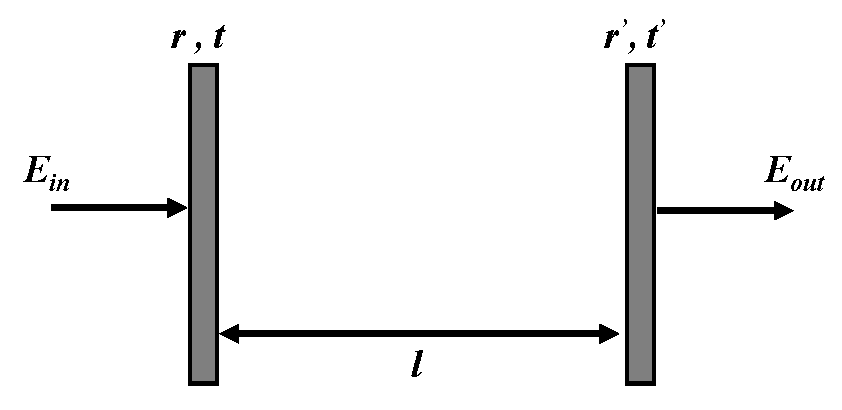
\includegraphics[width=0.6\textwidth]{figures/planar_fabry_perot.pdf}
    \caption{Sketch of a planar Fabry-Perot cavity.}
    \label{fig:planar_fabry-perot}
\end{figure}

The two mirrors are described by each their respective reflectivity \emph{r} and transmission \emph{t} and are placed parallel at a distance \emph{l} from each other. The field at the second mirror, i.e. the transmitted field $E_{out}$ can then be described as a function of the field at the first mirror, i.e. the incident field $E_{in}$\cite{Eichhorn} \cite{Pedrotti}. The Fabry-Perot cavity furthermore gives rise to so-called eigenstates related to it's length \emph{l}, derived from considering the path difference between succesive parallel beams throught the cavity. Any allowed mode inside the cavity, and thus transmitted, must fulfill the brightness condition $2l = m \lambda$, where $\lambda$ is the wavelength of the incident field and $m=1,2,3,...$ is a positive integer.  

\subsubsection{Transmission}

In order to determine the transmission throught the Fabry-Perot interferometer, we once again consider the configuration in figure \ref{fig:planar_fabry-perot}. It is further, initially, assumed that resonators are both lossless, such that
\begin{equation}
    |r|^2 + |t|^2 = |r^{\prime}|^2 + |t^{\prime}|^2 = 1.
    \label{eq:lossless_condition}
\end{equation}

This means that all losses, e.g. absorption, are neglected. 

In order to formulate the field transmitted at the 2nd mirror $E_{out}$ in terms of the incident field at the 1st mirror $E_{in}$, we first consider the incident field as a propagating plane-wave
\begin{equation}
    E_{in} = E_{0,in} e^{ik},
\end{equation}

where $k = 2 \pi / \lambda$ is the wave number and $E_{0,in}$ is the amplitude of the field. We then consider $E_{out}$ to be comprised of contributions for each roundtrip inside the cavity. This can be written as an infinite geometrical series given as
\begin{equation}
    \begin{split}
        E_{out} & = tt^{\prime} E_{0,in} e^{ik} + tt^{\prime} E_{0,in} e^{ik} rr^{\prime} e^{i\delta}\\&+ tt^{\prime} E_{0,in} e^{ik} \left(rr^{\prime} e^{i\delta}\right)^2 + tt^{\prime} E_{0,in} e^{ik} \left(rr^{\prime} e^{i\delta}\right)^3 + ...\\& = tt^{\prime} E_{0,in} e^{ik} \sum^{\infty}_{m=0}\left( rr^{\prime}e^{i\delta} \right)^m
    \end{split}
    \label{eq:transmission_as_geometric_series}
\end{equation}
where $\delta = 2kl$. The first term of the series corresponds to a direct transmission through the cavity, and each term thereafter corresponds to the respective contribution to the transmission after the $m'th$ round trip. 

By evaluating the series it is seen that it converges to the final expression for the transmitted field through a planar Fabry-Perot cavity found as
\begin{equation}
    E_{out} = E_{0,in}\frac{tt^{\prime} e^{i\delta /2}}{1 - rr^{\prime} e^{i\delta}}.
    \label{eq:fabry_perot_trans}
\end{equation}

The intensity of the transmission is now taken as the square of the norm of the field amplitude $|E_{out}|^2$ and normalizing with respect to the incident field intensity $|E_{0,in}|^2$ we arrive at an expression for the transmission intensity which is recognized to be given as an \emph{Airy function}\cite{Pedrotti}
\begin{equation}
    T = \frac{|E_{out}|^2}{|E_{0,in}|^2} = \left|\frac{tt^{\prime}e^{i\delta/2}}{1 - rr^{\prime}e^{i \delta}}\right|^2 = \frac{(1-|r|^2)(1-|r^{\prime}|^2)}{(1-|rr^{\prime}|)^2 + 4|rr^{\prime}|sin^2(\delta)},
    \label{eq:airy_function}
\end{equation}
where $\delta$ is the phase shift for each round trip inside the cavity.

\begin{figure}[h!]
    \centering
    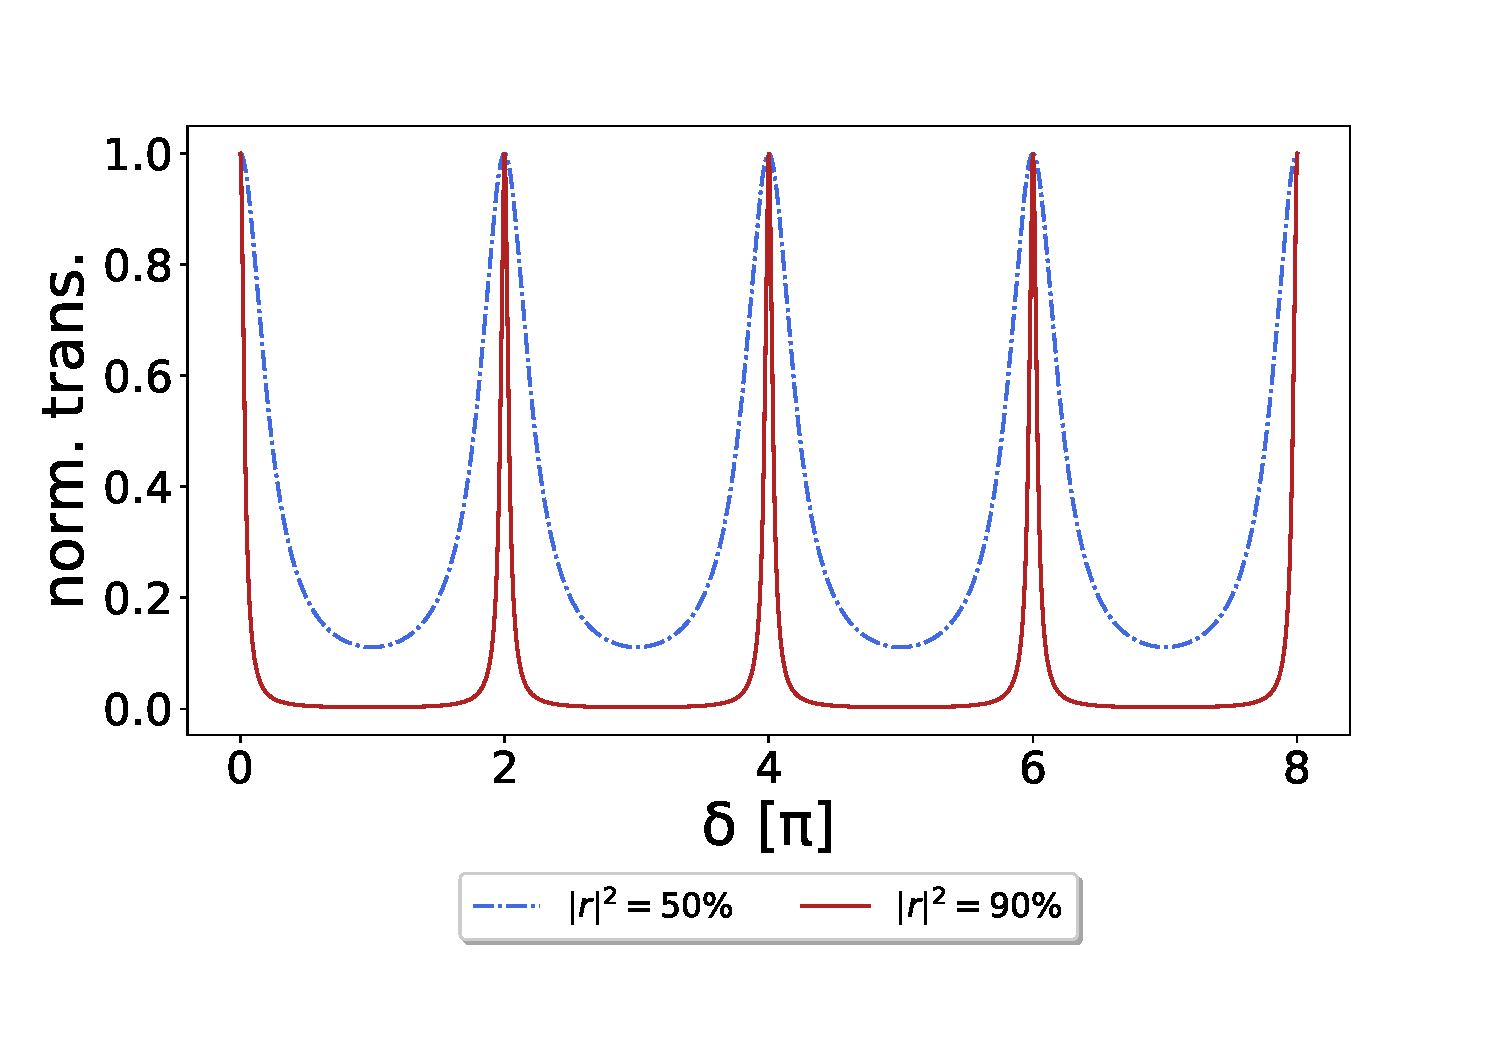
\includegraphics[width=0.7\textwidth]{figures/fabry_perot_high_and_low_finesse.pdf}
    \caption{The red line shows the transmission spectrum of a \emph{high} finesse Fabry-Perot cavity of reflectivity $|r|^2 = 0.90$, while the blue dashed line shows the transmission spectrum of a \emph{low} finesse cavity with reflectivity $|r|^2 = 0.50$.}
    \label{fig:fabry_perot_trans}
\end{figure}

Figure \ref{fig:fabry_perot_trans} displays the Airy function in eq. (\ref{eq:airy_function}), of a lossless cavity of reflectivities $r^{\prime} = r$, as a function of $\delta$ in units of $\pi$. The function is plotted for the cases of $|r|^2 = 50 \%$, shown in blue, and $|r|^2 = 90 \%$, shown in red. It is readily seen that the transmission is maximized for $\delta = n 2 \pi$ and that the two cases shown differ significantly as the red profile is much narrower than the blue. The red profile is hence said to have a higher \emph{finesse} $\mathcal{F}$ than the blue profile. The finesse is defined as
\begin{equation}
    \mathcal{F} \equiv \frac{FSR}{\delta_{\lambda}},
    \label{eq:finesse_definition}
\end{equation}
where $FSR$ is the so-called \emph{Free Spectral Range} indicating the spectral distance between two peaks and $\delta_{\lambda}$ refers to the \emph{Full Width at Half Maximum (FWHM)} which, as the name suggests, is the linewidth defined at $T=1/2$, i.e. at half the maximum value. 

Considering the Airy function in eq. (\ref{eq:airy_function}) for the high finesse case where $|r|^2 = |r^{\prime}|^2 \rightarrow 1$ we furthermore see that each individual peak resembles a Lorentzian distribution. 

\subsubsection{Varying the cavity length}

In order to relate the resonance transmission profile to the length of the cavity we first consider the frequencies at which the cavity is resonant, with respect to the incident light, given as
\begin{equation}
    \nu_n = n \frac{c}{2l},
    \label{eq:resonance_freq}
\end{equation}
where $c$ is the speed of light, $n$ is a positive integer refering to the order of the resonance frequency and $l$ is the cavity length. This corresponds to a peak occuring at times related to each round trip inside the cavity. 

Since the FSR is defined as the spectral distance between each peak, it follows from eq. (\ref{eq:resonance_freq}) that it can be be expressed in terms of the resonance frequencies as 
\begin{equation}
    FSR_{\nu} = \frac{c}{2l},
    \label{eq:FSR_vs_cavity_length}
\end{equation}
and the corresponding linewidth, or FWHM, $\delta_{\nu}$ is then given as
\begin{equation}
    \delta_{\nu} = \frac{1}{2 \pi} \frac{|t|^2 + |t^{\prime}|^2}{\tau},
\end{equation}
where $\tau = 2l/c$ is the round trip time in seconds. 

Finally, considering the definition of the finesse from eq. (\ref{eq:finesse_definition}) it can be shown that
\begin{equation}
    \mathcal{F} \equiv \frac{FSR_{\nu}}{\delta_{\nu}} = \frac{2 \pi}{|t|^2 + |t^{\prime}|^2},
    \label{eq:lossless_finesse}
\end{equation}
where the finesse is now defined in terms of the total cavity transmission at resonance. 

Note here that the relation between the FSR and the cavity length $l$ is clearly shown in eq. (\ref{eq:FSR_vs_cavity_length}), and figure \ref{fig:fabry_perot_FSR_comparison} furthermore shows transmission spectra underlining the effect of changing the cavity length. 

\begin{figure}[h!]
    \centering
    \begin{subfigure}[b]{0.49\textwidth}
        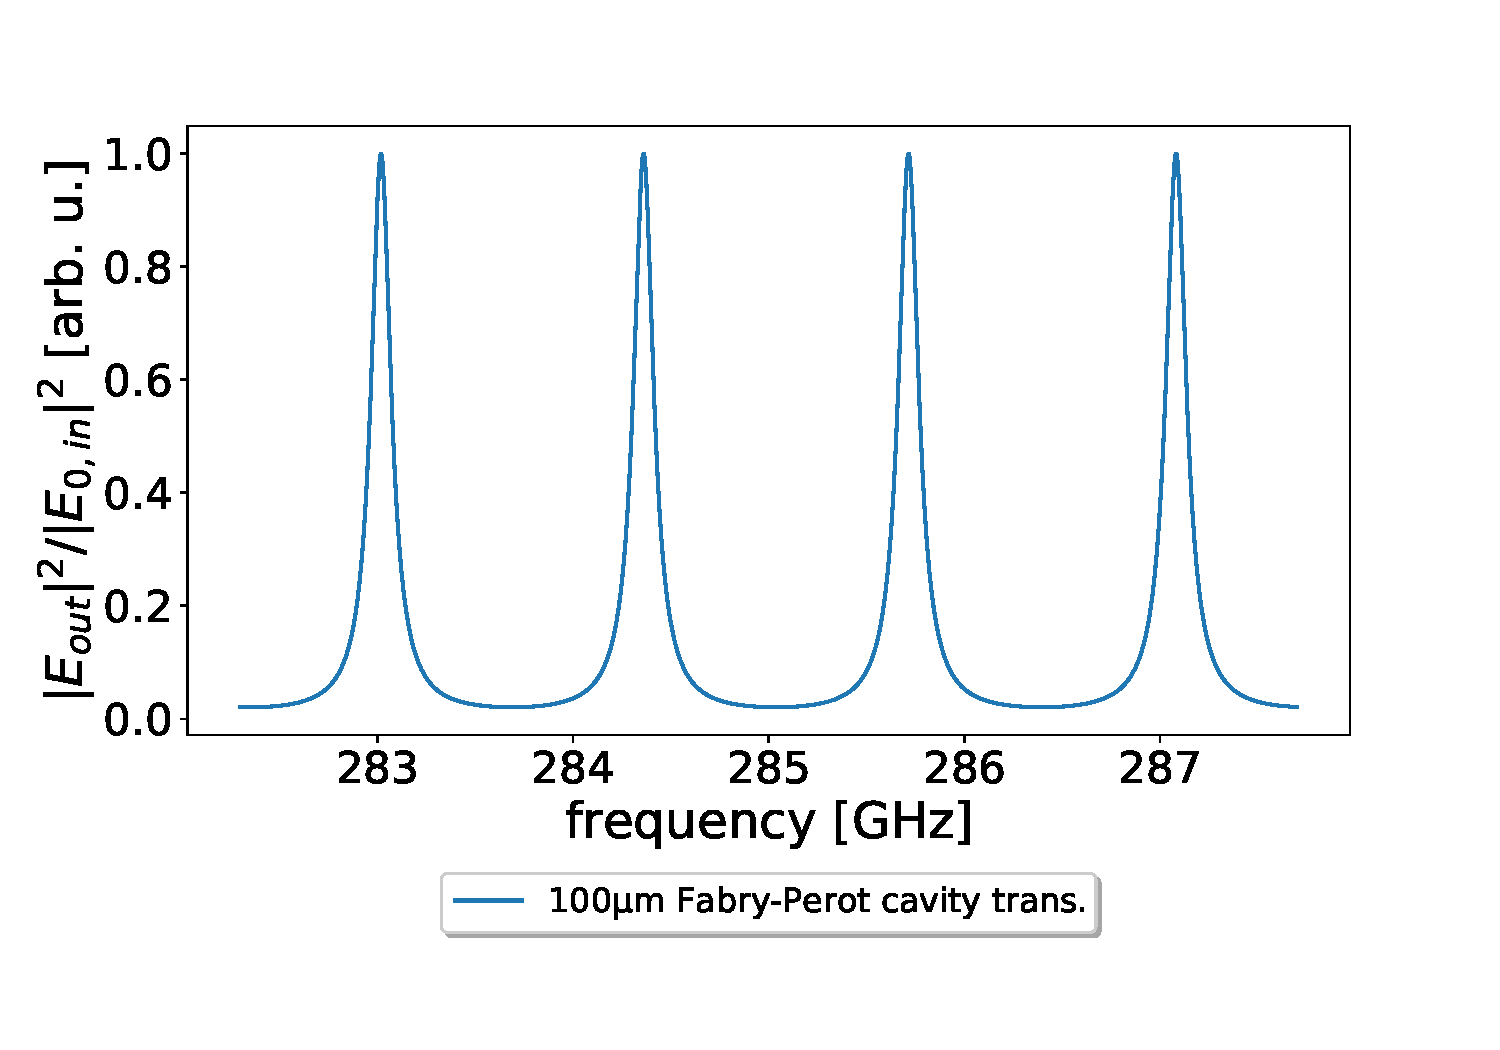
\includegraphics[width=\textwidth]{figures/100um_fabry_perot_trans_vs_freq.pdf}
        \caption{}
    \end{subfigure}
    \begin{subfigure}[b]{0.49\textwidth}
        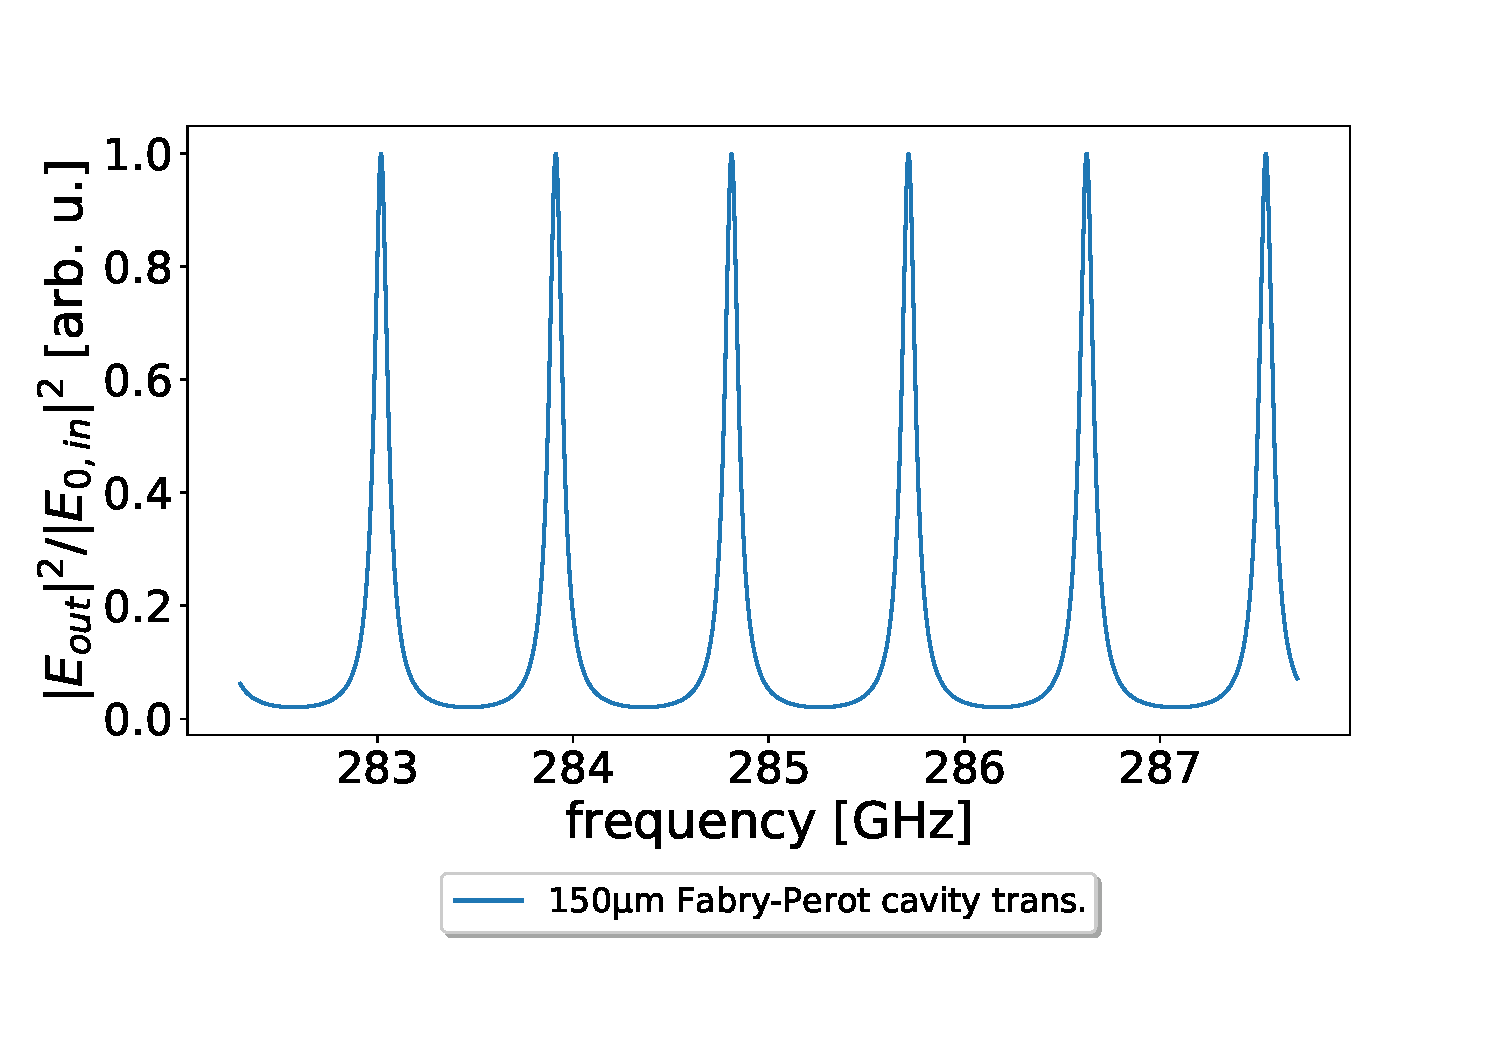
\includegraphics[width=\textwidth]{figures/150um_fabry_perot_trans_vs_freq.pdf}
        \caption{}
    \end{subfigure}
    \caption{(a) shows the transmission spectrum of a Fabry-Perot cavity of length $l \approx 100 \mu m$ as a function of the frequency $\nu$, while (b) shows the transmission spectrum of a cavity of length $l \approx 150 \mu m$ for the same range of frequencies. Note here how the FSR is invrsely proportional to the cavity length.}
    \label{fig:fabry_perot_FSR_comparison}
\end{figure}

\subsubsection{Varying the incident wavelength}

In order to simplify the Airy function in eq. (\ref{eq:airy_function}) we introduce the so-called \emph{coefficient of finesse} $F$, which is a function only of the mirror reflectivites, given as
\begin{equation}
    F = \frac{4 |rr^{\prime}|}{(1-|rr^{\prime}|)^2}.
\end{equation}

The coefficient of finess $F$ is not to be confused with the finesse $\mathcal{F}$. While the finesse is related to the sharpness of the transmission peaks, the coefficient of finesse refers to the contrast of the peaks in the sense that the difference between the minimum and maximum transmitance level increases with $F$. The coefficient of finesse is related to the finesse as 
\begin{equation}
    \mathcal{F} = \frac{\pi}{2} \sqrt{F}.
\end{equation}

Rewriting the Airy function in terms of the coefficient of finesse yields
\begin{equation}
    T_{\lambda} = \frac{1}{1+ F sin^2 \left(\delta / 2\right)},
\end{equation}
where the round trip phase shift $\delta$ is related to the wavelength $\lambda$ of the incident light by
\begin{equation}
    \delta = 2kl = \frac{4 \pi l }{\lambda},
\end{equation}
as $k = 2 \pi / \lambda$ is the incident wave number.

Re-writing the general cavity brightness condition, it can be shown that the resonant wavelengths for a cavity at normal incident are given as
\begin{equation}
    \lambda_n = \frac{2l}{n},
\end{equation}
where $n=1,2,3,...$ is a positive integer refering to the order of the resonance. 

Since $\nu = c / \lambda$, the relation between the linewidth in wavelength space $\delta_{\lambda}$ and the one in frequency space $\delta_{\nu}$ is non-linear. Therefore one does not simply make the aforementioned substitution in order to relate them. It can however be shown that their respective expressions differ by a factor of $\lambda^2/c$, and the linewidth when varying the wavelength is thus given as
\begin{equation}
    \delta_{\lambda} = \frac{\lambda^2}{c} \cdot \delta_{\nu} = \frac{\lambda^2}{4 \pi l} (|t|^2 + |t^{\prime}|^2).
\end{equation}
Finally we consider the definition for the finesse $\mathcal{F}$ and the expression given in eq. (\ref{eq:lossless_finesse}), in order to show that the $FSR$ in wavelength space is given as 
\begin{equation}
    FSR_{\lambda} = \delta_{\lambda} \cdot \mathcal{F} =  \frac{\lambda^2}{2l}.
\end{equation}



\begin{figure}[h!]
    \centering
    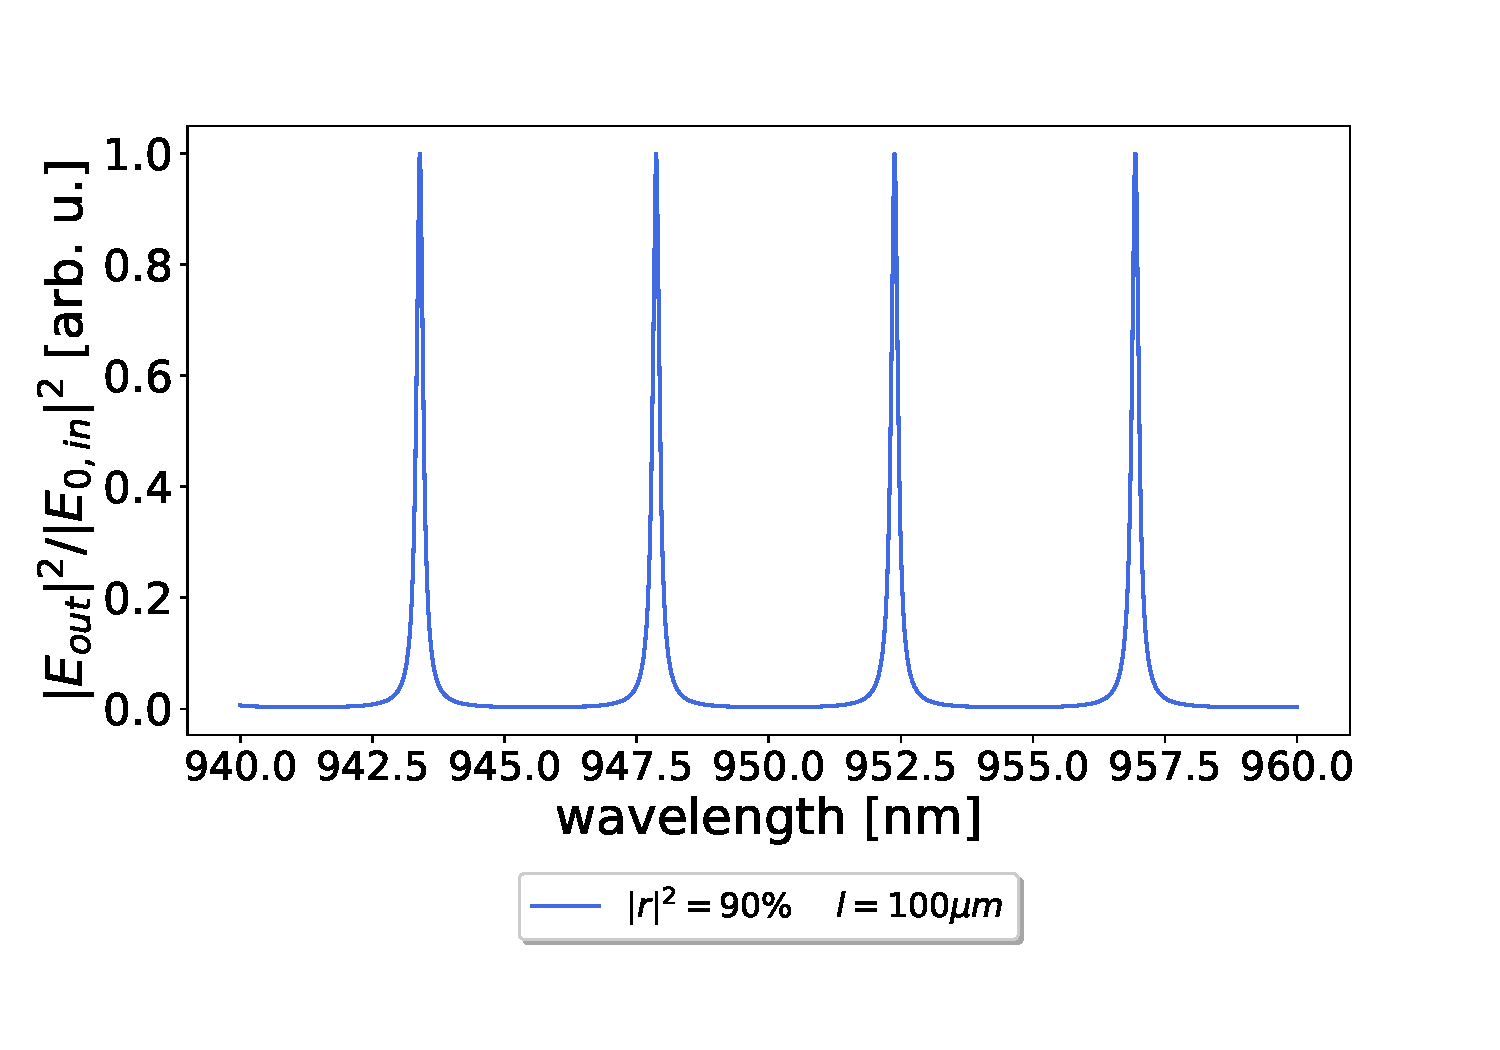
\includegraphics[width=0.7\textwidth]{figures/airy_function_vs_wavelength.pdf}
    \caption{}
    \label{fig:airy_trans_vs_wavelength}
\end{figure}

\subsubsection{Cavity losses}

In eq. (\ref{eq:lossless_finesse}) we assume the case of a lossless cavity, i.e. eq. (\ref{eq:lossless_condition}) is fulfilled. In practice, any cavity will have some amount of losses, which would have to be taken into account when calculating the finesse. When losses are present eq. (\ref{eq:lossless_condition}) instead generally reads
\begin{eqnarray}
    |r|^2 + |t|^2 + L + L^{\prime} = 1,
\end{eqnarray}
where $L$ and $L^{\prime}$ indicates the fractional losses of each resonator.

In this case the finesse would be given as 
\begin{equation}
    \mathcal{F} = \frac{2 \pi}{|t|^2 + |t^{\prime}|^2 + L_{total}},
\end{equation}
where $L_{total} = L + L^{\prime}$ are the total cavity losses.

The effect on the transmission spectrum of a cavity with losses is that the level of the normalized transmission will not reach unity, as some light is lost to i.g. absorption or scattering for each round trip of the cavity.

\subsection{The Fano mirror: a sub wavelength grating}\label{sec:fano_mirror}

\subsubsection{Reflection/transmission spectra and line shape analysis}

\subsubsection{Lossless grating}

We wish to analytically describe the wavelength-dependent spectra for the transmission and reflectivity of an infinite sub-wavelength grating. The wavelength dependence arises from the fact that any incident light will be subject to interactions with the so-called \emph{guided-mode} of the grating. The grating is, in this way, said to act as an effective $\text{TM}_0$ waveguide, ensuring resonant modes will only be reflected in the 0'th order. 

By first considering the case where absorption and thermal coupling effects are neglected, i.e. a lossless grating, we can assume conservation of energy and thereby the relations
\begin{equation}
    |r_g|^2+|t_g|^2=1 \hspace{0.5cm} \text{and} \hspace{0.5cm} |r_d|^2+|t_d|^2=1,
    \label{eq:energy conservation}
\end{equation}
where the subscripts \emph{g} and \emph{d} indicate the \emph{grating} and \emph{direct} transmissions and reflectivities, respectively. It is implied that the direct coefficients are constants and describe the transmission and reflectivity when the incident wavelength is significantly detuned from any guided-mode resonance of the grating. Furthermore, it is also implied that the grating coefficients are functions of the incident wavelength.

We now assume a normal incident beam on the grating as a linearly polarized monochromatic plane wave, with a wavelength close to a guided-mode resonance of the grating. In order to describe the coefficients $r_g$ and $t_g$ we follow the formalism presented by Fan and Joannopoulos \cite{Fan-Joannopoulos-guided-mode-resonance} and consider the likely paths of the incident light through the grating. It is quite intuitive to consider the case where the light is simply transmitted, and this shall be our first case hereafter denoted the \emph{direct pathway}. Another case one might consider is the one where the incident light excites the guided-mode resonance in the grating. This case is denoted the \emph{indirect pathway} and decays more slowly than it's direct counterpart. 

The interference caused when the guided mode is excited is often referred to as \emph{Fano resonances}, due to its physical similarities to the description of interference between a discrete autoionized state and a bound continuum state first reported by Fano \cite{Fano-theory}. The cross section of inelastic scattering, when measured as a function of energy, showed characteristic asymmetric peaks. These were described as the aforementioned interference pattern between \emph{direct} (the discrete state) and \emph{indirect} (the continuum state) pathways. 

By generalizing the model of Fan and Joannopoulos \cite{Fan-Joannopoulos-guided-mode-resonance} we describe the transmission and reflectivity coefficent amplitudes as 
\begin{equation}
    r_g = r_d + \frac{a}{k-k_1 + i\gamma} \hspace{0.5cm} \text{and} \hspace{0.5cm} t_g = t_d + \frac{b}{k-k_1+i\gamma},
    \label{eq:ref/trans}
\end{equation}
where $k=2\pi/\lambda$ is the incident wave number, $k_1 = 2\pi/\lambda_1$ is the wave number according to the guided-mode resonance and $\gamma$ is the HWHM (half width at half maximum) of the guided-mode resonance. Complex coefficients $a$ and $b$ describe the interference between the directly transmitted or reflected waves and the guided mode of the grating. 

Note that in eq. (\ref{eq:ref/trans}) the right side of the expression for each coefficient corresponds to the continuum state i.e. the indirect pathway, while the direct transmission and reflection coefficients take the role of the autoionized discrete state, i.e. the direct pathway\cite{Fano-theory}.

As we are dealing with an ideal, lossless, grating, we assume coefficients $a$ and $b$ to be equal, meaning that we specifically assume vertical symmetry throughout the grating. By considering eq. (\ref{eq:energy conservation}) this in turn leads to 
\begin{equation}
    a = b = -i \gamma (t_d + r_d),
\end{equation}
which further yields an expression for the grating transmission amplitude coefficient on the form
\begin{equation}
    t_g = t_d \frac{k - k_0}{k - k_1 + i \gamma}.
    \label{eq:lossless transmission coefficient}
\end{equation}
Here, the newly introduced $k_0 = 2\pi/\lambda_0 = k_1 -i \gamma (r_d/t_d)$ is the zero-transmission/unity-reflectivity wave number.

To generalize eq. (\ref{eq:lossless transmission coefficient}) to include non-unity reflectivity and non-zero transmission, we allow for $a \neq b$\cite{Bykov}\cite{Darki2}\cite{Parthenopoulos}, meaning that the case of vertical asymmetry is included in the model\cite{Popov}. By assuming $r_d,t_d \in \mathbb{R}$, eq. (\ref{eq:energy conservation}) leads to the coupled differential equations
\begin{equation}
    \begin{split}
        &t_d x_a + r_d x_b = 0, \hspace{0.3cm} \text{and} \\
        &x_a^2 + y_a^2 + x_b^2 + y_b^2 + 2 t_d \gamma y_a + 2 r_d \gamma y_b = 0,
    \end{split}
    \label{eq:lossless couples diff. eqs.}
\end{equation}
where $\{x,y\}_{a,b}$ respectively denotes the real and imaginary parts of the coefficients $a$ and $b$. Solving eqs. (\ref{eq:lossless couples diff. eqs.}) leads to the correct complex reflectivity coefficients and the expression for the transmission coefficient amplitudes now reads
\begin{equation}
    t_g = t_d \frac{k - k_0 + i \beta}{k - k_1 + i \gamma},
    \label{eq:transmission_coefficients_non_zero_values}
\end{equation}
where $k_0$ and $\beta$ are defined from the expression for $a$ found by solving eqs. (\ref{eq:lossless couples diff. eqs.}), given as
\begin{equation}
    a = t_d (k_1 - k_0 - i \gamma + i \beta).
\end{equation}
Finally, this allows for non-zero transmission and non-unity reflectivity at wave number $k_0$.

To show the validity of the model at this point, we introduce a periodic grating which is arbitrarily sketched in figure \ref{fig:MIST_grating_sketch}. The sketch indicates the period of the grating $\Lambda$, the top finger width $w_t$, the offset between the finger top and the bottom of the grating $x$, the total grating thickness $t$ and finger depth $d$. Furthermore, the grating is patterned on a \emph{silicon nitride (SiN)} membrane  of refractive index $n_{SiN}$. 

\begin{figure}[h!]
    \centering
    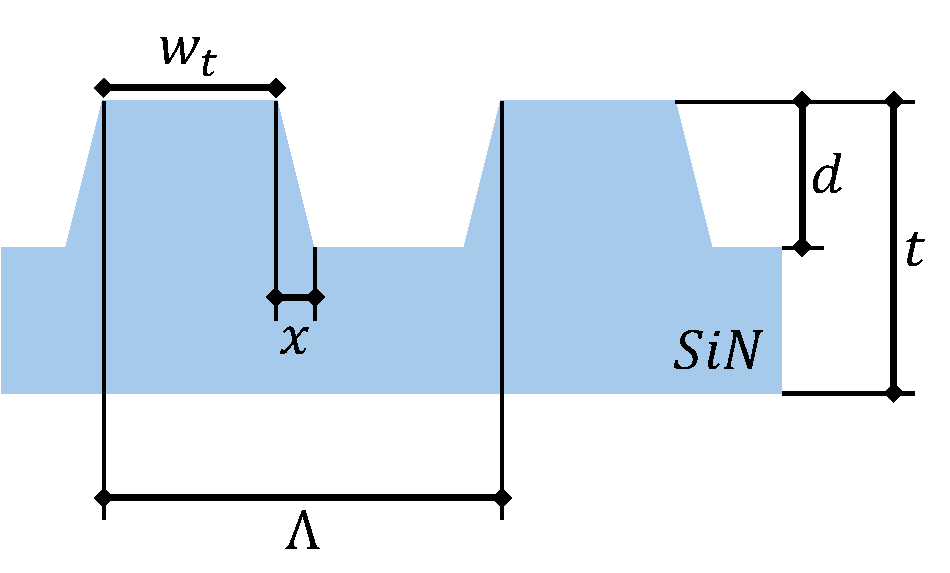
\includegraphics[width=0.7\textwidth]{figures/grating_MIST_sketch.pdf}
    \caption{Schematics of a periodic optical $SiN$ grating with phyiscal parameters: $\Lambda = 857$nm, $w_t = 623$nm, $h = 55.1$nm, $t = 152$nm, $d = 67$nm, $n_{SiN} = 2.15$.}
    \label{fig:MIST_grating_sketch}
\end{figure}


In order to simulate the transmission and reflectivity profiles as a function of the incident wavelength, we utilize the \emph{Modeled Integrated Scatter Tool (MIST)} developed by the \emph{National Institute of Standards and Technology (NIST)}\cite{MIST}. The simulation solves Maxwell's equations for any pre-defined infinite periodic structure. 

MIST assumes an incident plane-wave, and hence predicts the \emph{ideal} spectra for the transmission and reflectivity, i.e. zero and unity when on resonance, respectively. In order to include effects related to the Gaussian behaviour of a more realistic incident beam, such as collimation and finite-size effects\cite{Toft-Vandborg}, one would have to solve Maxwell's equations for a Gaussian distribution. We safely assume an incident plane-wave for reasons related to the order of magnitude for the \emph{Rayleigh range} of the beam used, compared with that of the spacial range of the conducted experiments.

In reality, the interference inside the cavity however cannot be perfect, as any Gaussian beam can be represented by a number rays, infinitesimal in size, which would all track differently through the grating, resulting in non-unity reflectivity and non-zero transmission. In order to synthetically correct for this we scale each transmission value found by MIST according to
\begin{equation}
    t_g = (1 - \varepsilon) \cdot t_{MIST} + \varepsilon,
    \label{eq:trans_correction_MIST}
\end{equation}
where we define the correction to be arbitrarily small as $\varepsilon = 1\%$.

\begin{figure}[h!]
    \centering
    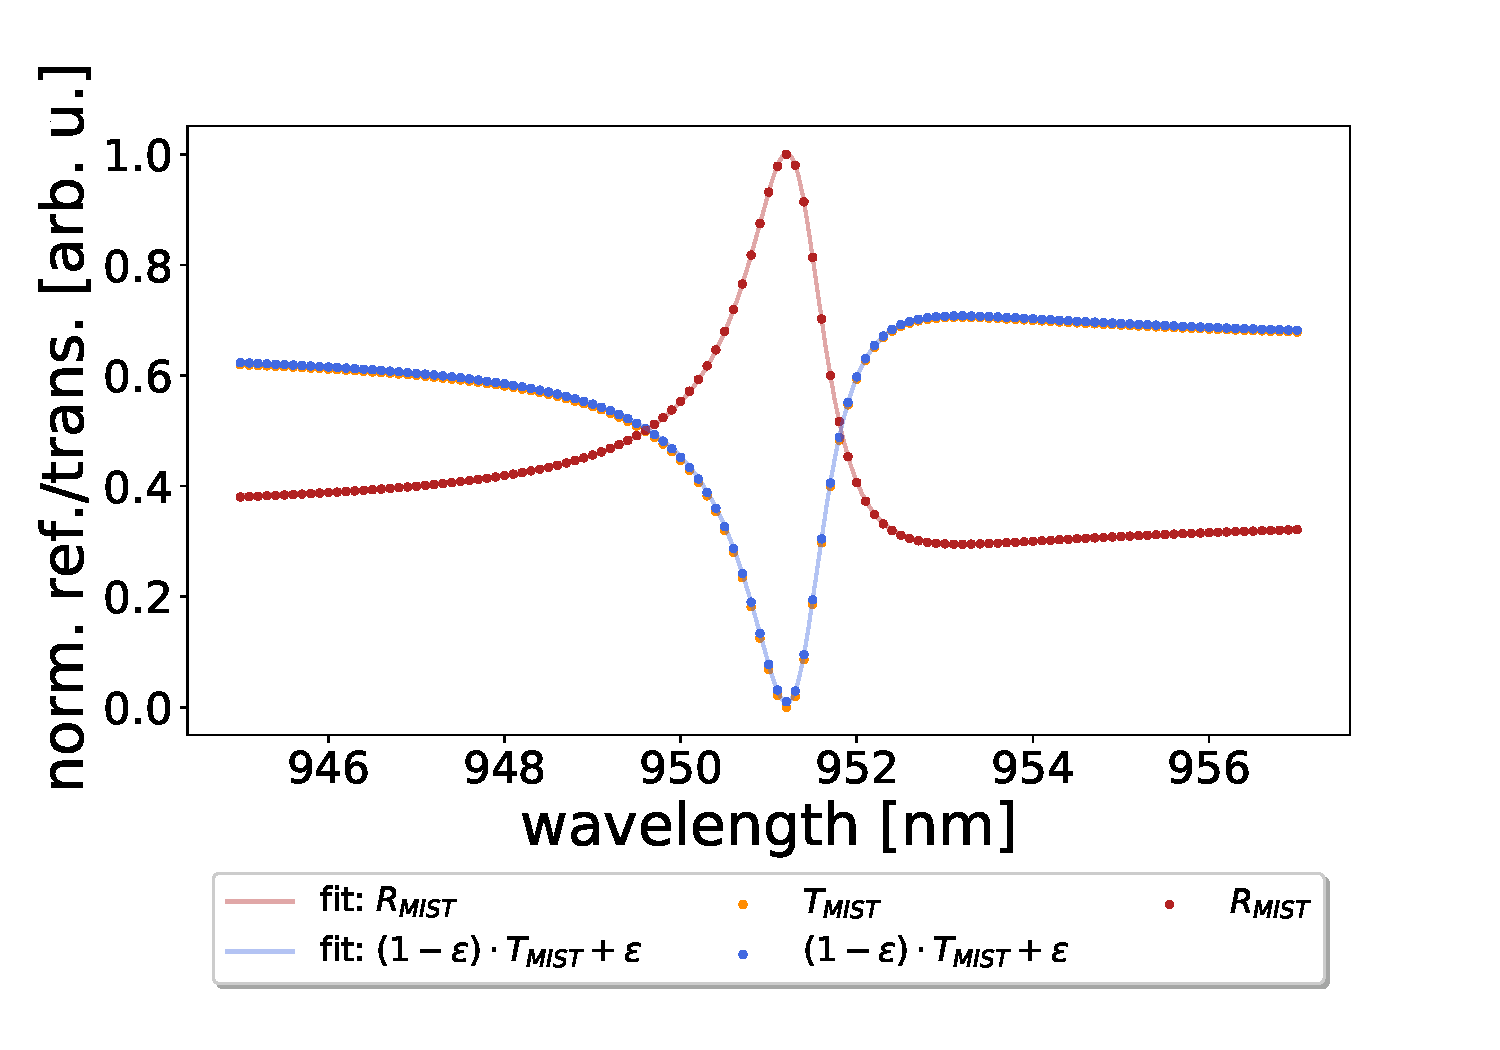
\includegraphics[width=0.7\textwidth]{figures/MIST_grating_sim.pdf}
    \caption{Reflectivity and transmission values (scaled and unscaled) found from a MIST simulation plotted with the corresponding least squares fit to the model in eq. (\ref{eq:transmission_coefficients_non_zero_values}). The resulting grating parameters are given as $\lambda_0 = 951.217$nm, $\lambda_1 = 951.356$nm, $t_d = 0.818$, $r_d = 0.527$, $\gamma_{\lambda} = 0.527$nm, and $\beta = 1.03 \cdot 10^{-6}$.}
    \label{fig:MIST_sim_of_grating}
\end{figure}

Figure \ref{fig:MIST_sim_of_grating} shows the scaled and unscaled results of the simulation using MIST for the following physical grating parameters:
\begin{equation}
    \begin{split}
    &\Lambda = 857 \text{nm},\:\: w_t = 623 \text{nm},\:\: h = 55.1 \text{nm},\\ &t = 152 \text{nm},\:\: d = 67 \text{nm}\: \text{ and }\: n_{SiN} = 2.15,
    \end{split}
    \label{eq:physical_grating_params}
\end{equation}

The reflectivity- and (corrected) transmission values were then fitted to the model in eq. (\ref{eq:transmission_coefficients_non_zero_values}) using a least squares fitting method, and plotted along with the simulated values. The resulting grating parameters were found as
\begin{equation}
    \begin{split}
    &\lambda_0 = 951.208 \text{nm},\:\: \lambda_1 = 951.356 \text{nm},\:\: t_d = 0.8094,\\ &r_d = 0.527,\:\: \gamma_{\lambda} = 0.527 \text{nm}\: \text{ and }\: \beta = 4.42 \cdot 10^{-7},
    \end{split}
    \label{eq:optical_grating_params}
\end{equation}
where $\lambda_0$ is the cavity mode resonance wavelength, $\lambda_1$ is the guided-mode resonance wavelength, $r_d$ ($t_d$) is the direct reflectivity (transmission), $\gamma_{\lambda}$ is the width of the guided-mode resonance and $\beta$ is a constant associated with non-unity reflectivity and non-zero transmission. 

\subsubsection{Lossy grating}

In order to modify the above model such that losses, e.g. due to absorption or thermal coupling effects, are accounted for, we add a resonant loss term to the energy conservation relation in eq. (\ref{eq:energy conservation}). For this we introduce the resonant loss level $L$, which must be known in order to accurately calculate the complex reflectivity coefficients. The energy conservation relation is modified such that
\begin{equation}
    |t_g|^2 + |r_g|^2 + \frac{c^2}{(k - k_1)^2 + \gamma^2} = 1,
    \label{eq:lossy energy conservation}
\end{equation}
where the coefficient $c^2 = L((k-k_1)^2 + \gamma^2)$ includes the resonant loss term $L$. A new set of coupled differential equations are found, using eq. (\ref{eq:lossy energy conservation}), given as
\begin{equation}
    \begin{split}
        &t_d x_a + r_d x_b = 0, \hspace{0.3cm} \text{and} \\
        &x_a^2 + y_a^2 + x_b^2 + y_b^2 + c^2 +  2 t_d \gamma y_a + 2 r_d \gamma y_b = 0.
    \end{split}
    \label{eq:lossy couples diff. eqs.}
\end{equation}
It is easily identified that eq. (\ref{eq:lossless couples diff. eqs.}) and eq. (\ref{eq:lossy couples diff. eqs.}) differ only by the addition of coefficient $c^2$, and thereby the losses. Solving eq. (\ref{eq:lossy couples diff. eqs.}) leads to the correct complex reflectivity coefficients, except that they now account for any losses associated with the grating. 

In conclusion, the complete grating model consists of an expression for the transmission coefficients and a set of coupled differential equations for the reflection coefficients, shown in eq. (\ref{eq:transmission_coefficients_non_zero_values}) and eq. (\ref{eq:lossy couples diff. eqs.}), respectively. The model on the form used for this project and subsequent thesis is derived in previous work by A. Darki et al. \cite{Darki} and more recently T. Mitra et al. \cite{Mitra}.

Figure \ref{fig:lossy_grating_spectrum} shows reflection and transmission spectra of a grating of parameters given in eq. \ref{eq:optical_grating_params} with a synthetic non-zero resonance loss term in order to show the effect of including losses. It is seen from the added \emph{loss curve} that the losses increase when approaching the resonance wavelength, as the interaction with the guided-mode, and thus the grating, gets stronger in this region. 
\begin{figure}[h!]
    \centering
    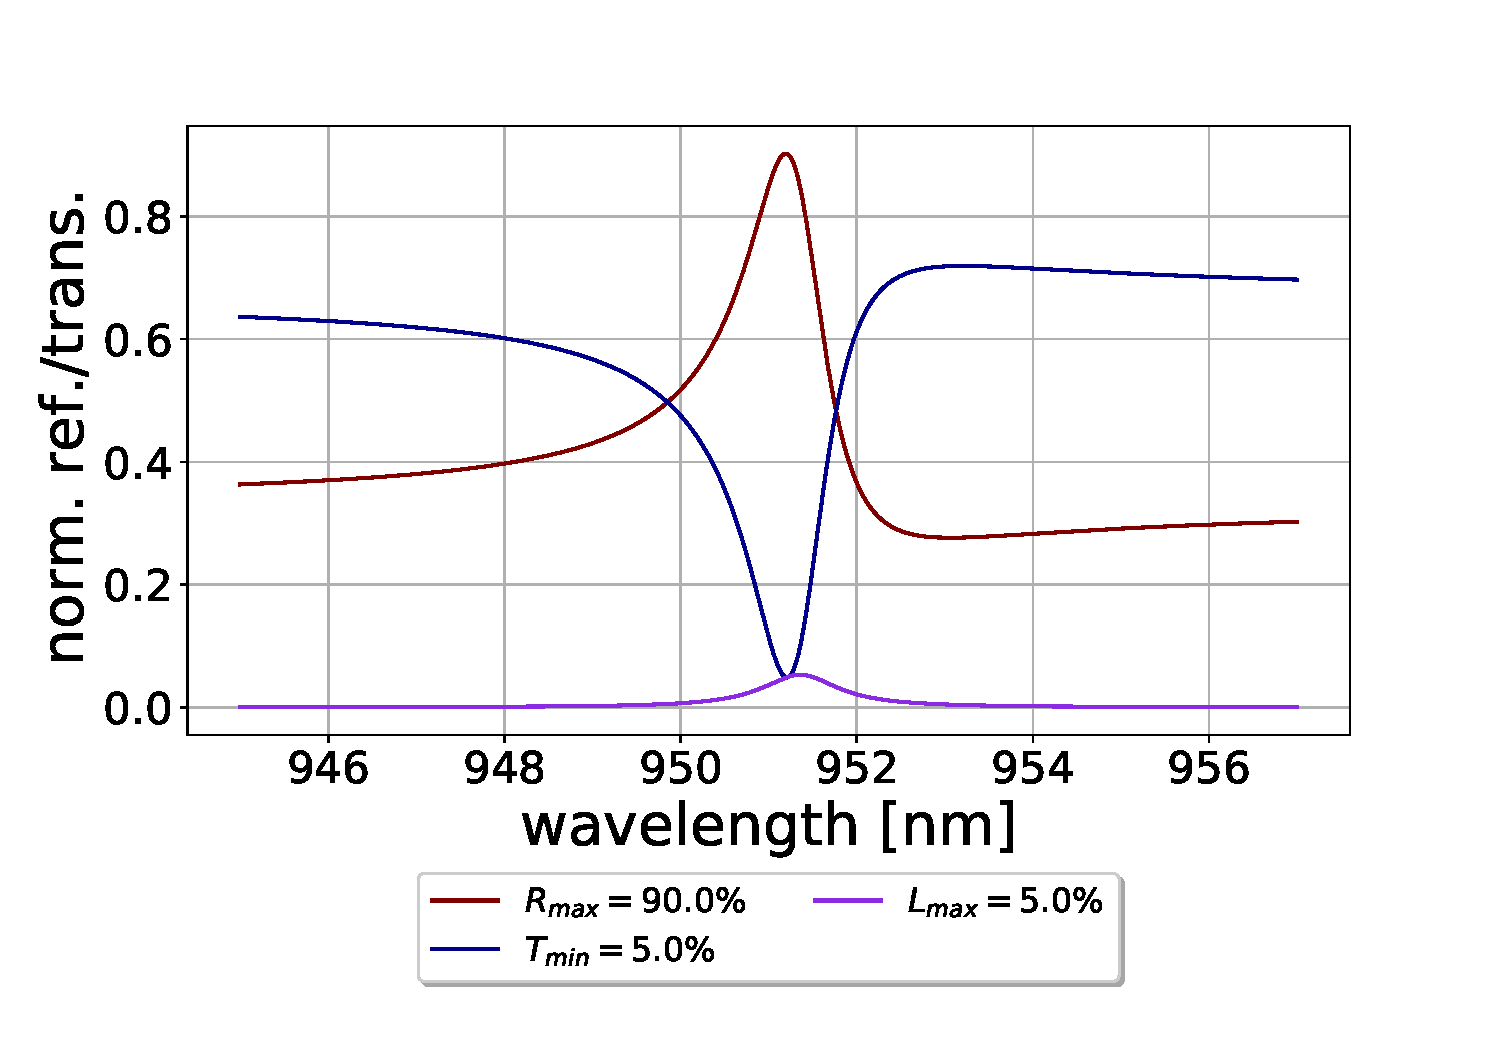
\includegraphics[width=0.7\textwidth]{figures/arbitrary_lossy_grating_ref_trans.pdf}
    \caption{Simulated reflectiviy and transmission spectra of a grating of parameters given in eq. (\ref{eq:optical_grating_params}) with a synthetically added non-zero resonant loss term. The purple line indicate the corresponding grating losses.}
    \label{fig:lossy_grating_spectrum}
\end{figure}

\subsection{The single Fano cavity}

\subsubsection{The single Fano cavity model}

The single Fano cavity consists of a planar broadband mirror, and a sub-wavelength grating, i.e. a Fano mirror, as described in section \ref{sec:fano_mirror} and seen in figure \ref{fig:broadband_and_single_fano_sketch} where schematics of the single Fano and broadband cavity configurations are shown. While the broadband mirror has fixed optical properties, the Fano mirror has transmission and reflection coefficients dependent on the incident wavelength, according to solutions to the coupled differential equations of eq. (\ref{eq:lossy couples diff. eqs.}). 

\begin{figure}[h!]
    \centering
    \begin{subfigure}[b]{0.3\textwidth}
        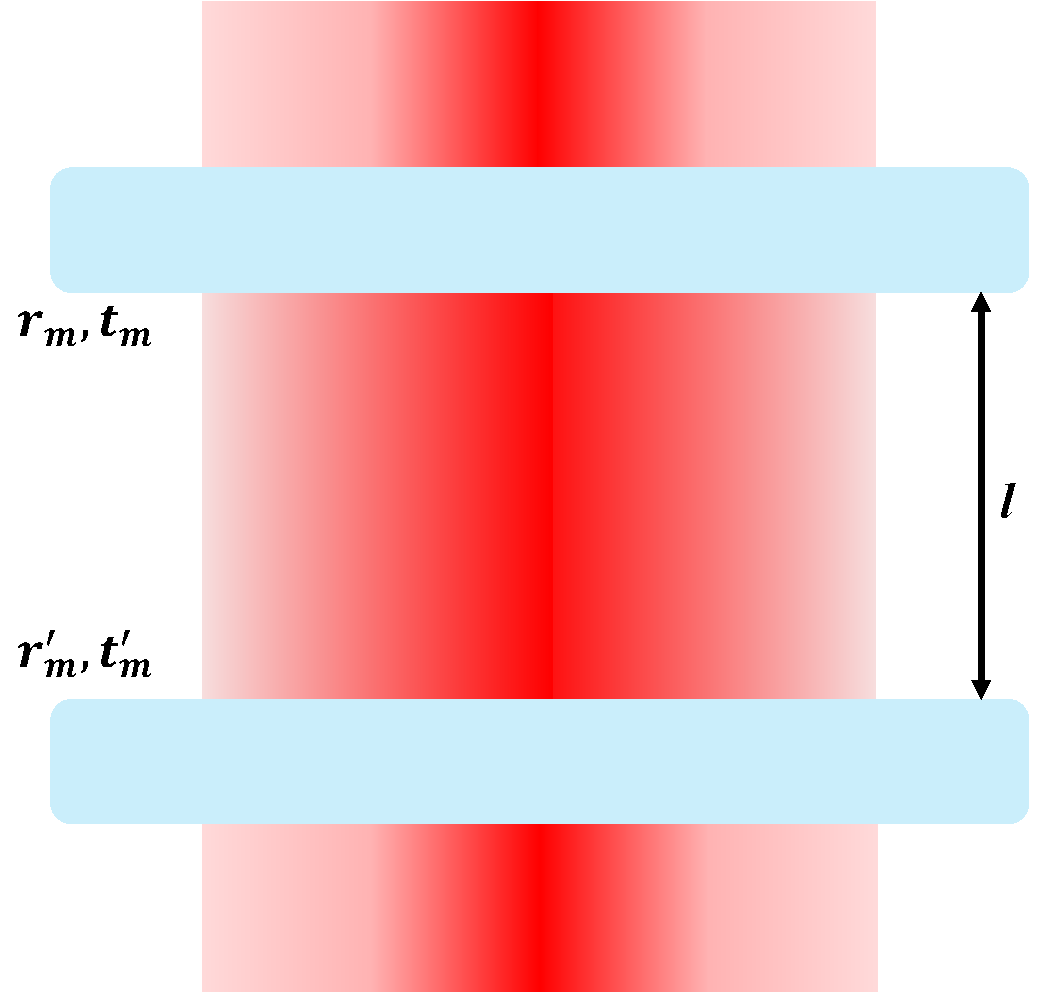
\includegraphics[width=\textwidth]{figures/broadband_sketch.pdf}
        \caption{}
        \label{fig:broadband_sketch}
    \end{subfigure}
    \hspace{1cm}
    \begin{subfigure}[b]{0.3\textwidth}
        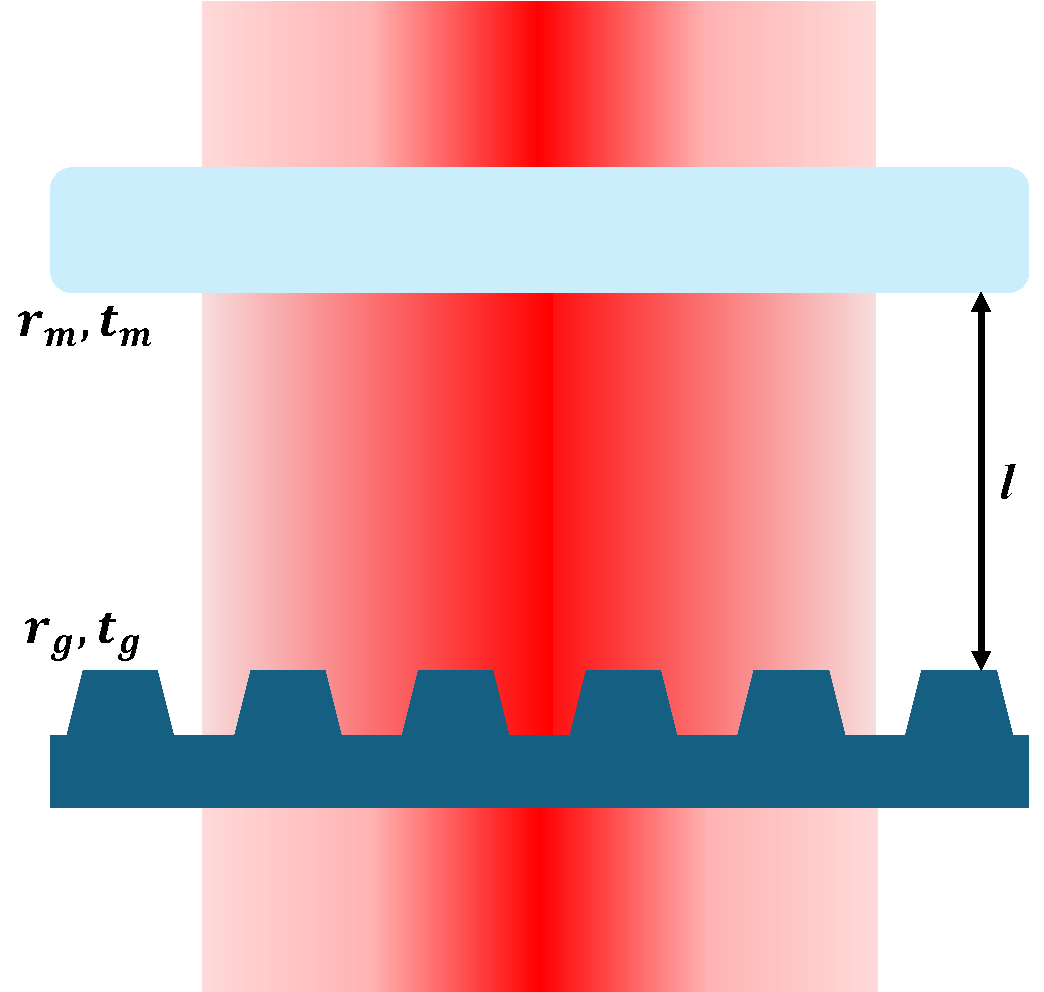
\includegraphics[width=\textwidth]{figures/single_fano_sketch.pdf}
        \caption{}
        \label{fig:single_fano_sketch}
    \end{subfigure}
    \caption{In (a) is seen the schematics of a cavity consisting of two broadband mirrors with transmission and reflectivity coefficients $t_m$, $r_m$, $t_m^{\prime}$, and $r_m^{\prime}$. (b) shows the schematics of a single Fano cavity consisting of one broadband mirror with coefficients $t_m$, $r_m$ and one Fano mirror with wavelength dependent coefficients $t_g$, $r_g$. The reflectors in either cavity are separated by a cavity length $l$.}
    \label{fig:broadband_and_single_fano_sketch}
\end{figure}

In order to model the single Fano cavity transmission spectra, we therefore consider the transmission function of a normal incident and planer Fabry-Perot cavity in eq. (\ref{eq:fabry_perot_trans}) with $r,t \rightarrow r_m,t_m$ and $r^{\prime},t^{\prime} \rightarrow r_g(\lambda),t_g(\lambda)$\cite{Naesby}. Here the subscript $m$ indicates the broadband \emph{mirror} coefficients, and $g$ is for \emph{grating}, which indicates the coefficients of the Fano mirror. Rewriting eq. (\ref{eq:fabry_perot_trans}) such that it describes the normalized transmission amplitude, through the single Fano cavity, $T_{cav} = |E_{out}|^2/|E_{0,in}|^2$ we get
\begin{equation}
    T_{cav} = \left|\frac{t_m t_g(\lambda) e^{i\phi}}{1 - r_m r_g e^{2i\phi}}\right|^2,
    \label{eq:single_fano_trans}
\end{equation}
where $\phi = 2\delta = kl$, $k=2 \pi / \lambda$ and $l$ is the cavity length, as is consistent with the general case described in section \ref{sec:fano_mirror}.

\subsubsection{Transmission linewidth}\label{sec:single_fano_cavity_trans_linewidth}

We aim to analytically describe how the transmission spectrum at, or close to, the overall resonance behaves as a function of the incident wavelength. The overall resonance is the term used for the case of $\lambda_g \approx \lambda_c \approx \lambda_l$, where $g,c,l$ stands for grating/guided-mode, cavity and laser, respectively, and the Fano model is hence generalized for this specific scenario. Considering the case where the cavity resonance closely resembles the guided-mode resonance of the Fano mirror (the zero-transmission wavelength), eq. (\ref{eq:single_fano_trans}) can be approximated well by
\begin{equation}
    T_{cav} \approx \frac{A}{1 + \left( \frac{\Delta}{1 - \nu \Delta} \right)^2},
    \label{eq:general_fano_model}
\end{equation}
where $\Delta = (\lambda - \lambda_c) / \delta \lambda$ is the detuning from the cavity resonance normalized by the HWHM $\delta \lambda$, and $\nu$ is a constant describing the asymmetry of the single Fano transmission spectrum. \cite{Mitra}\cite{Darki} 

From eq. (\ref{eq:general_fano_model}) it can be shown that the HWHM of the Fano transmission profile around the overall resonance wavelength, i.e. when $\lambda_c \approx \lambda_0$, is approximately given as
\begin{equation}
    \delta \lambda \approx \frac{1}{\frac{1}{\delta \lambda_c} + \frac{1}{\delta \lambda_g}},
    \label{eq:analytical_linewidth}
\end{equation}
where 
\begin{equation}
    \delta \lambda_c = \frac{\lambda_0^2}{8 \pi l} (|t_g(\lambda_0)|^2 + |t_m|^2 + L)
    \label{eq:analytical_linewidth_broadband}
\end{equation}
is the HWHM of a broadband cavity and
\begin{equation}
    \delta \lambda_g = \frac{\gamma_{\lambda}}{2 (1-r_d)}(|t_g(\lambda_0)|^2 + |t_m|^2 + L)
    \label{eq:analytical_linewidth_single_fano}
\end{equation}
is the HWHM of the Fano cavity in the so-called Fano regime.\cite{Mitra}\cite{Darki} In eqs. (\ref{eq:analytical_linewidth})-(\ref{eq:analytical_linewidth_single_fano}) $\lambda_0$ is the Fano cavity resonance wavelength, $l$ is the cavity length, $L = \left(1 - |r_g(\lambda_0)|^2 - |t_g(\lambda_0)|^2\right)$ is the total additional losses of the cavity when on resonance, $\gamma \lambda$ is the width of the guided-mode resonance of the Fano mirror and $r_d$ is the off-resonance, or \emph{direct}, reflectivity of the Fano mirror.

The \emph{Fano regime} and its counterpart the so-called \emph{standard regime} are defined for a given single Fano cavity, by its length $l$. By inspection of eqs. (\ref{eq:analytical_linewidth_broadband}) and (\ref{eq:analytical_linewidth_single_fano}) it is seen that for $l \rightarrow \infty$ the linewidth in eq. (\ref{eq:analytical_linewidth}) is dominated by the broadband cavity term, while for the opposite case, $l \rightarrow 0$, the linewidth is predominantly given by the Fano cavity term. 

Generally the Fano regime describes the cavity lengths for which eq. (\ref{eq:analytical_linewidth}) shows a significant divergence from the broadband linewidth in eq. (\ref{eq:analytical_linewidth_broadband}). Oppositely, when in the standard regime the broadband and Fano cavity produces resonance transmission peaks of comparable, if not equal, linewidths.

We now introduce a single Fano cavity consisting of the Fano mirror introduced in section \ref{sec:fano_mirror} and sketched in figure \ref{fig:MIST_grating_sketch}, and a broadband mirror of reflectivity $|r|^2=90\%$ and transmission $|t|^2=1\%$. Figures \ref{fig:standard_regime_trans} and \ref{fig:fano_regime_trans} depicts examples of the transmission spectra in the standard and Fano regimes together with their respective complimentary broadband cavity transmission profiles. The reflectiviy amplitude of the Fano mirror is shown in both figures.

\begin{figure}[h!]
    \centering
    \begin{subfigure}[b]{0.49\textwidth}
        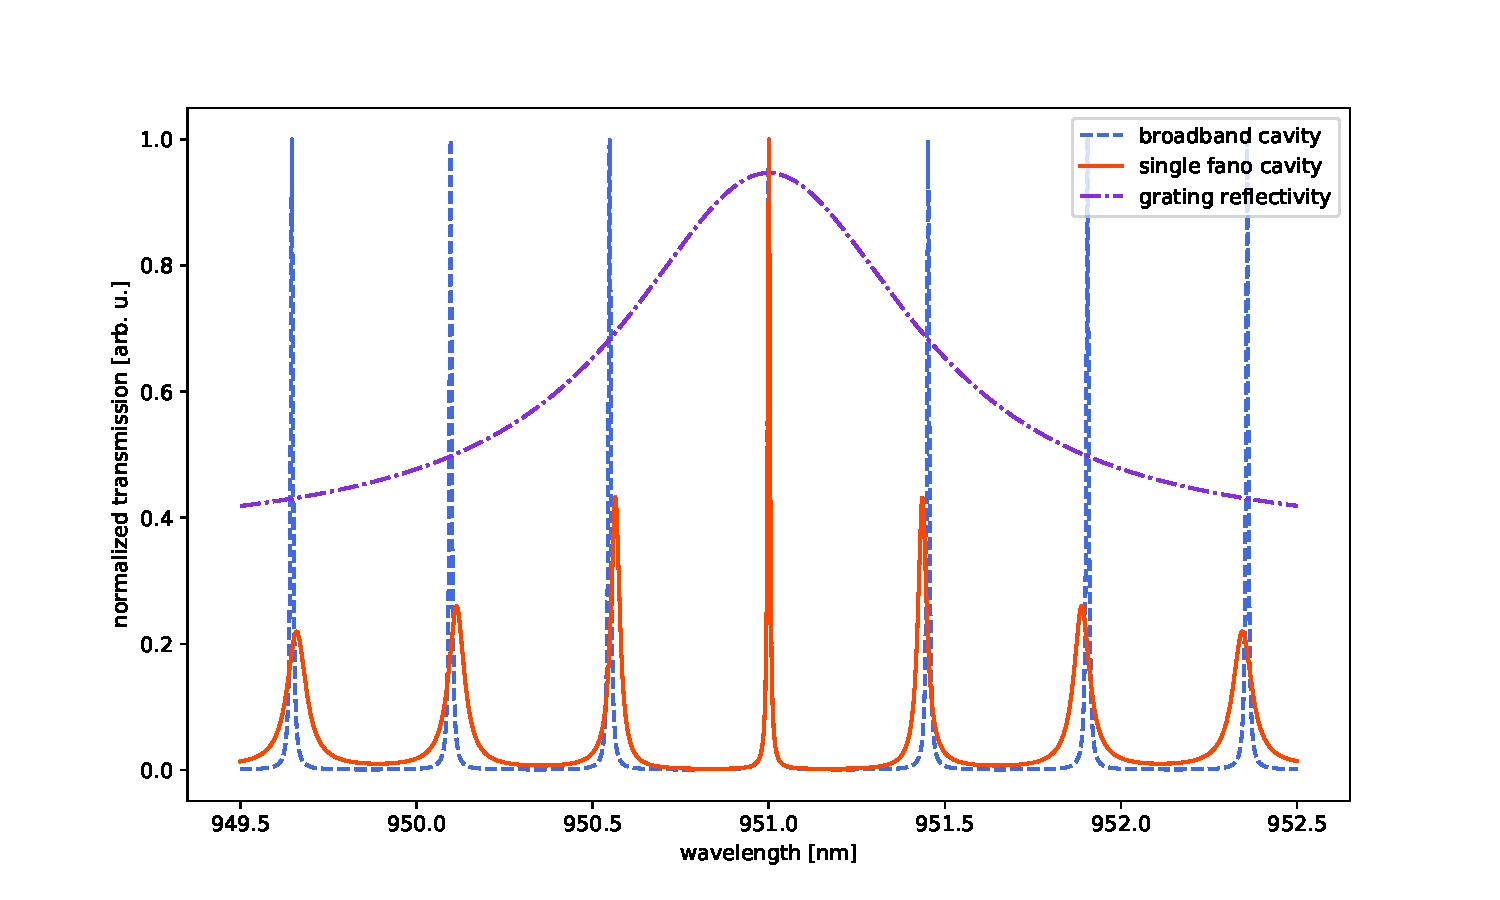
\includegraphics[width=\textwidth]{figures/fano_and_broadband_cavity_1000um.pdf}
        \caption{}
        \label{fig:standard_regime_trans}
    \end{subfigure}
    \begin{subfigure}[b]{0.49\textwidth}
        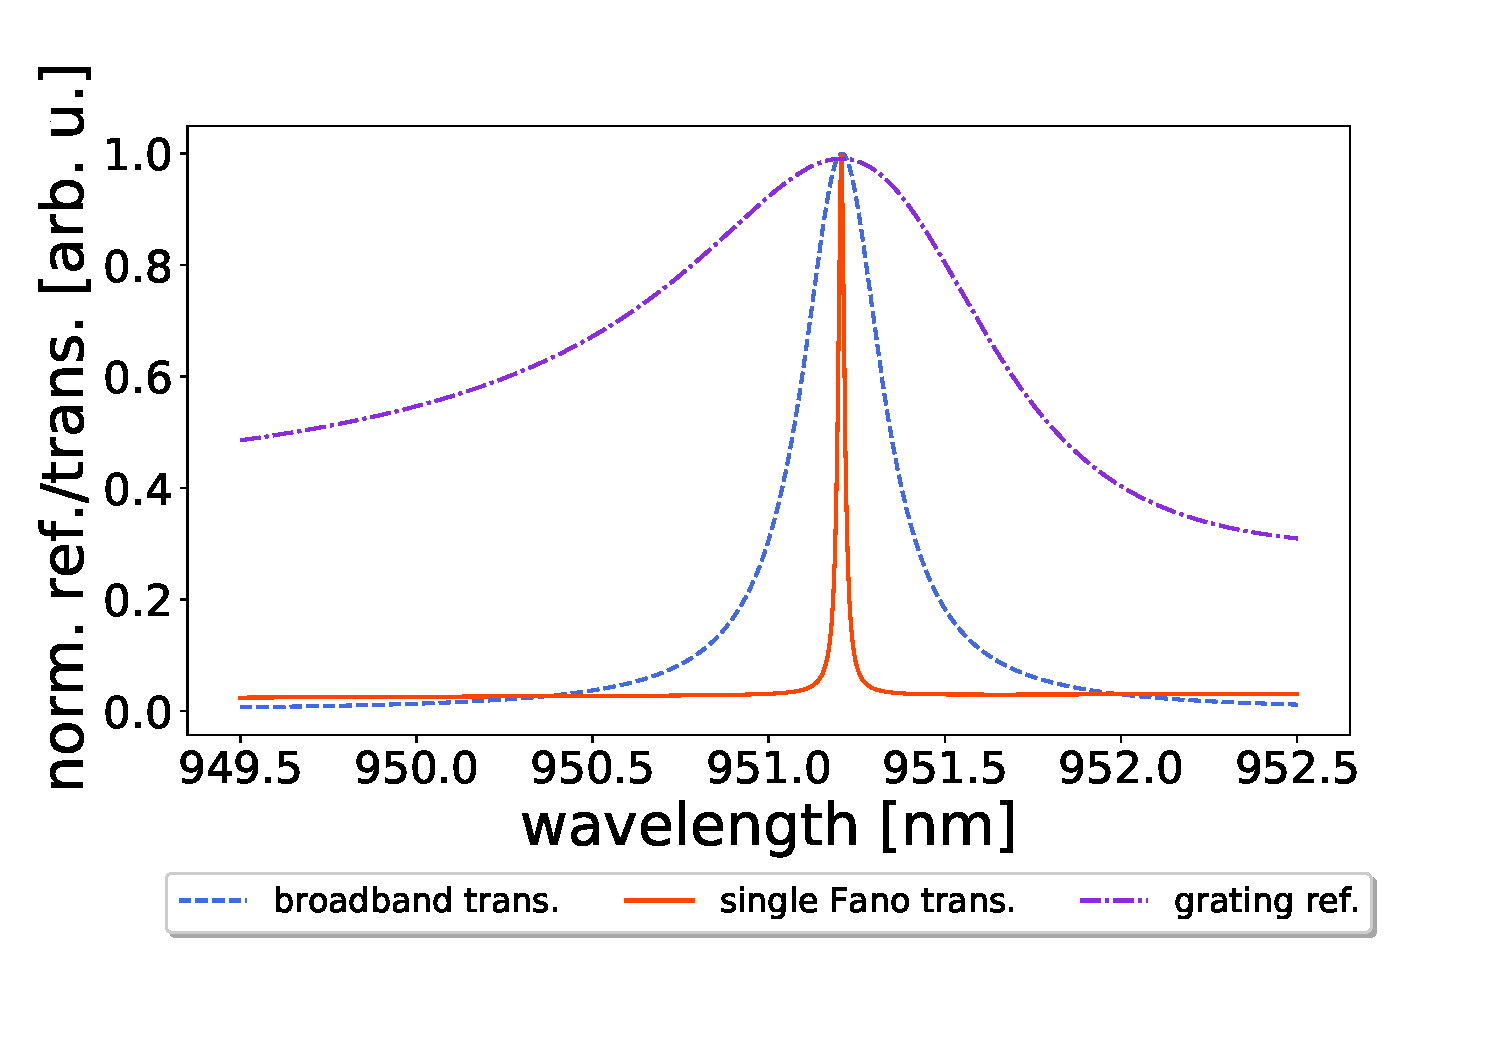
\includegraphics[width=\textwidth]{figures/fano_and_broadband_cavity_5um.pdf}
        \caption{}
        \label{fig:fano_regime_trans}
    \end{subfigure}
    \caption{In (a) is seen the comparison of broadband and single Fano cavity transmission spectra for a cavity length of $l \approx 1000 \mu m$, i.e. in the \emph{standard} regime. (b) shows the same comparison, but for a cavity length of $l \approx 5 \mu m$, i.e. in the so-called \emph{Fano} regime.}
\end{figure}

Figure \ref{fig:standard_regime_trans} shows the transmission spectra of the two cavities for a length of $l \approx 1000\mu m$, i.e. in the standard regime. It is clear from inspection of the figure that the resonance transmission profile of the standard broadband cavity is not wavelength dependent, in the sense that all fringes appear to have the same high finesse $\mathcal{F}$, i.e. ratio between the FSR and HWHM. This is not the case for the Fano cavity which is due to the wavelength dependence of the optical properties of the Fano mirror, as this causes the transmission and reflectivity to \emph{only} match those of the broadband mirror when on resonance. Furthermore, no significant difference in linewidth is seen for the transmission of the two cavities on resonance, as predicted by eq. (\ref{eq:analytical_linewidth}).

In figure \ref{fig:fano_regime_trans}, the transmission spectra of both cavities are shown for a length of $l\approx 5 \mu m$, i.e. in the Fano regime. Here it is clearly seen that while the standard cavity, as expected, experiences broadening for shorter cavity lengths, this is not the case for the Fano cavity transmission peak.

\begin{figure}[h!]
    \centering
    \begin{subfigure}[c]{0.7\textwidth}
        \centering
        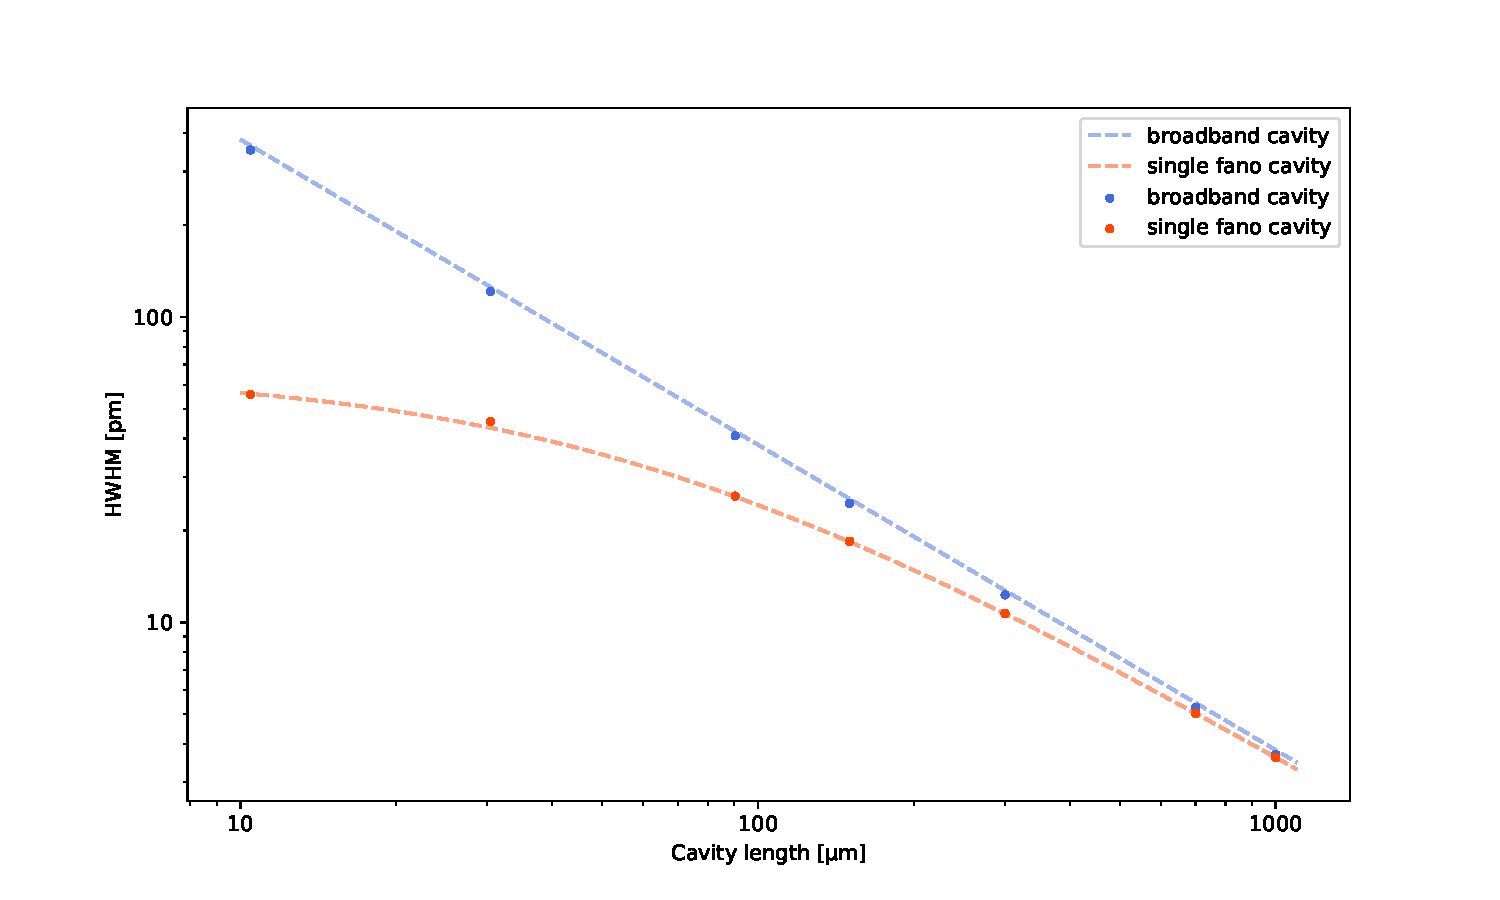
\includegraphics[width=\textwidth]{figures/HWHM_broadband_vs_single_sim.pdf}
        \caption{}
        \label{fig:HWHM_broadband_vs_single_fano}
    \end{subfigure}
    \begin{subfigure}[c]{0.49\textwidth}
        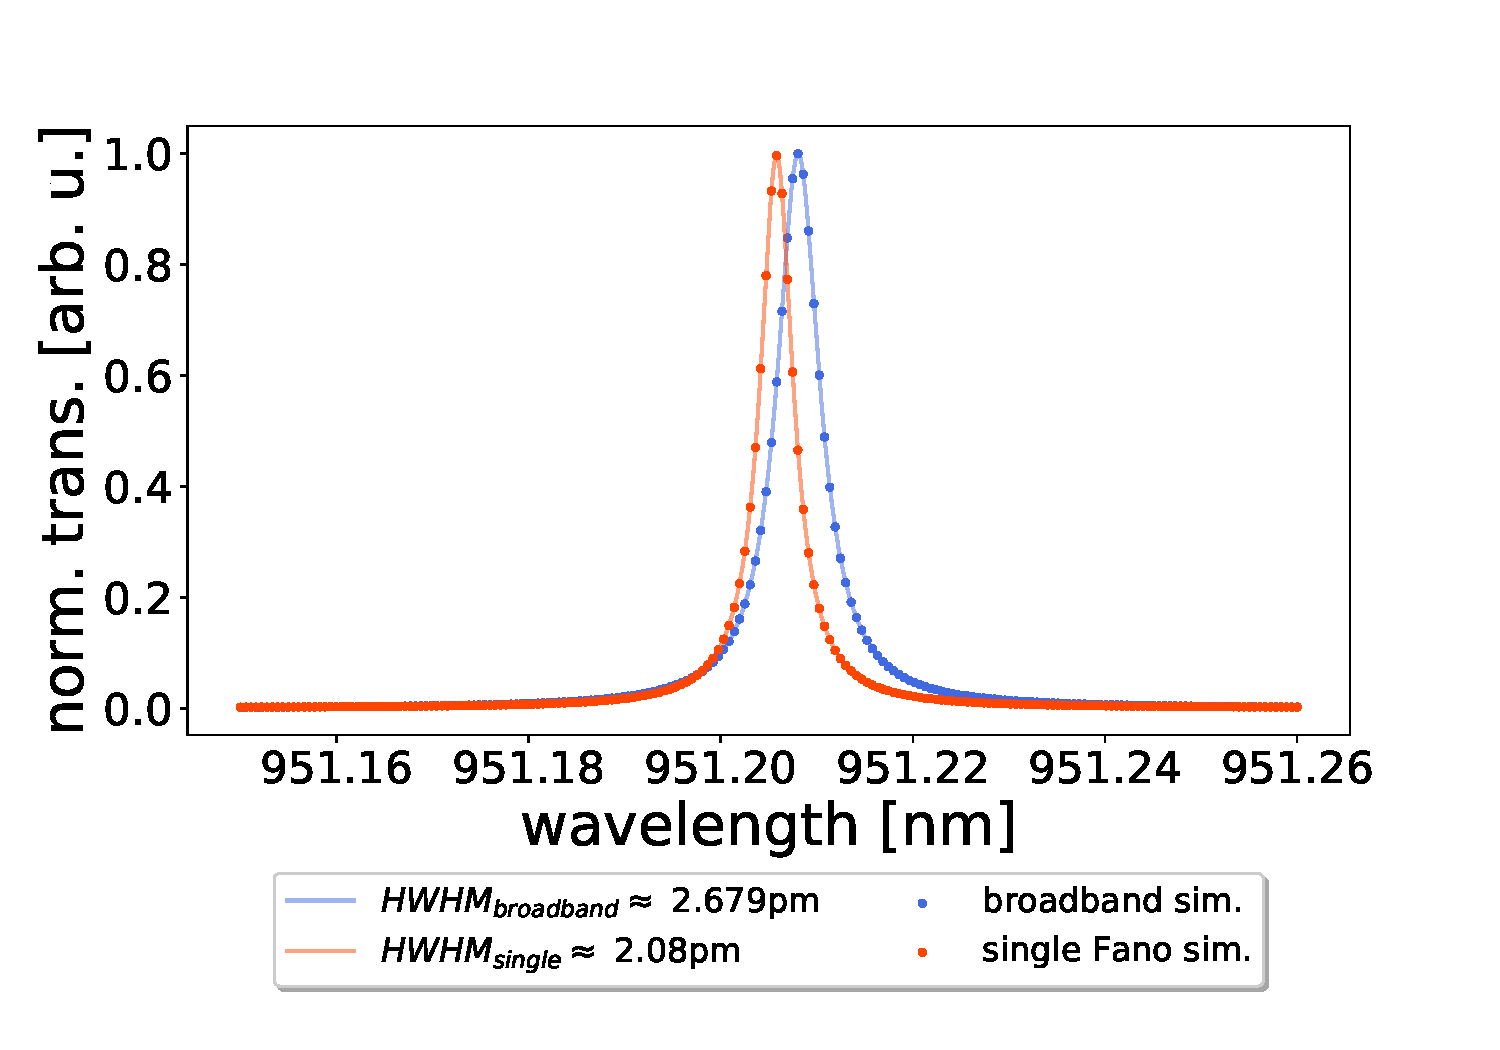
\includegraphics[width=\textwidth]{figures/sim_single_vs_broadband_270um.pdf}
        \caption{}
        \label{fig:270um_broadband_and_single_fano_peak}
    \end{subfigure}
    \begin{subfigure}[c]{0.49\textwidth}
        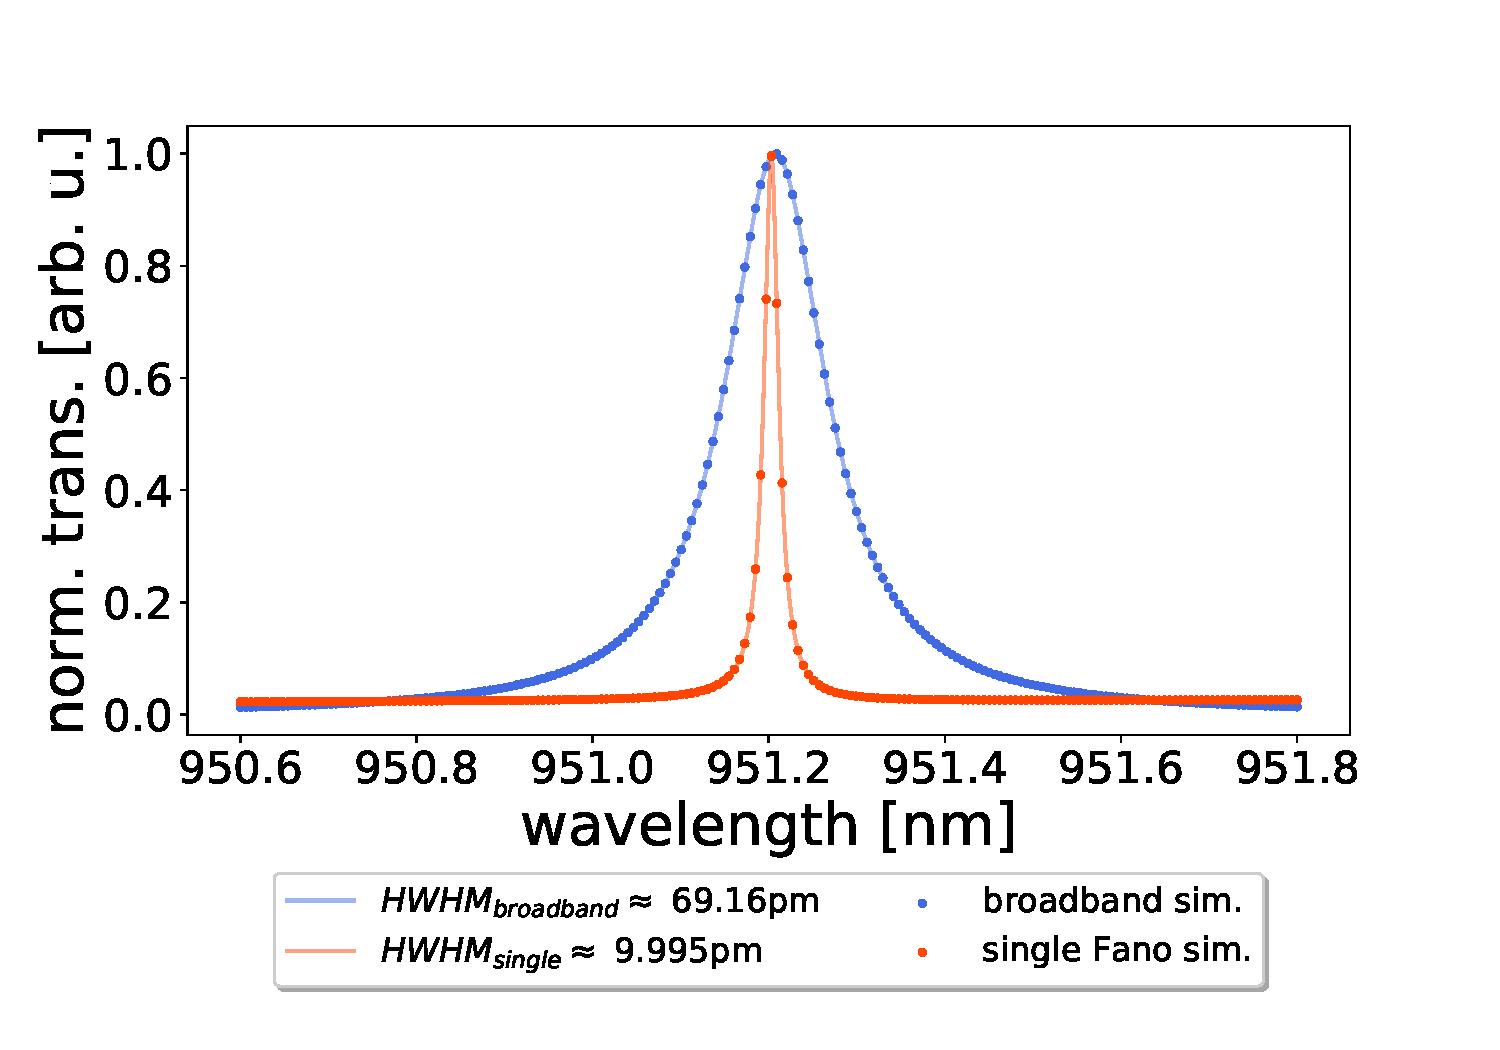
\includegraphics[width=\textwidth]{figures/sim_single_vs_broadband_10um.pdf}
        \caption{}
        \label{fig:10um_broadband_and_single_fano_peak}
    \end{subfigure}
    \caption{(a) shows the approximate analytical resonance linewidths (eq. (\ref{eq:analytical_linewidth})) as a function of cavity length for the broadband and single Fano cavities together with linewidths of transmission profiles simulated using eq. (\ref{eq:single_fano_trans}) and eq. (\ref{eq:fabry_perot_trans}), found as parameters of least squares fits, for comparison. In (b) and (c) is seen transmission spectra of broadband and single Fano cavities of lengths $\sim 270 \mu m$ and $\sim 10 \mu m$, respectively. The spectra shown indicate each their respective linewidths, and are examples of the values plotted in (a).}
\end{figure}

Figure \ref{fig:HWHM_broadband_vs_single_fano} models the behavior of the linewidth of the single Fano cavity compared with the one for a broadband cavity of similar optical properties, as a function of wavelength. Here it is easily seen where the linewidth of the single Fano transmission begins to saturate, and hence deviate from the one of the broadband cavity. The plotted line in the figure is calculated using eq. (\ref{eq:analytical_linewidth}) while the points depicit linewidths found as a fitting parameter from a least squares fit of the general Fano model in eq. (\ref{eq:general_fano_model}) to transmission spectra simulated by the Fabry-Perot (eq. (\ref{eq:fabry_perot_trans})) and single Fano (eq. (\ref{eq:single_fano_trans})) transmission functions. Finally, it can be concluded that the approximate analytical expression for the linewidth of the broadband and single fano cavities in eq. (\ref{eq:analytical_linewidth}) correlates very well with the values found from the simulated spectra.

\subsection{The double Fano cavity}

\subsubsection{The double Fano cavity model}

While the single Fano cavity is usually known in the appropriate litterature as simply a \emph{Fano cavity}, I have insisted on including the fact that it contains only one Fano mirror, and hence denoted it the \emph{single} Fano cavity. This addition is justified by the contents of this section, and namely that we now move on to the \emph{double} Fano cavity, which as the name suggests consists of two Fano mirrors. The schematics of this configuration is shown together with the one for the single Fano cavity in figure \ref{fig:single_and_double_fano_sketch}.

\begin{figure}[h!]
    \centering
    \begin{subfigure}[b]{0.3\textwidth}
        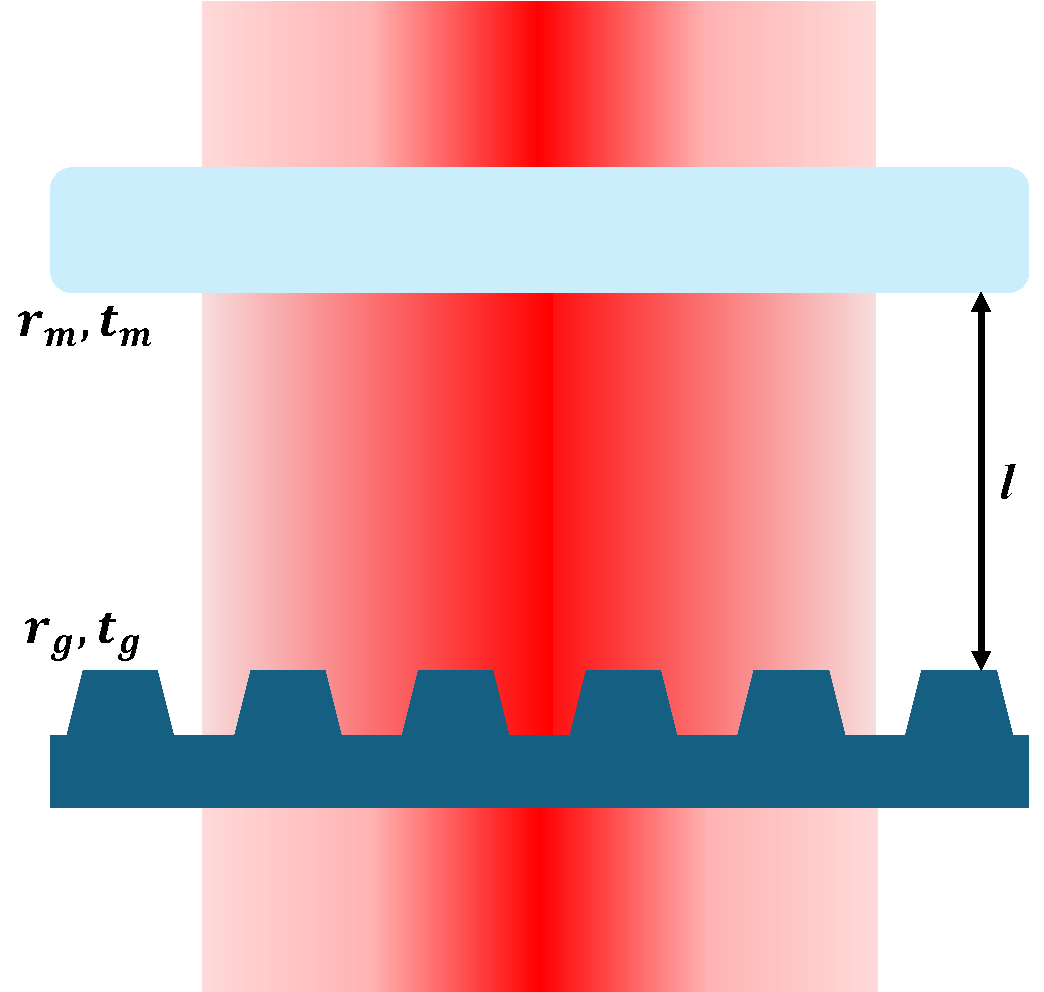
\includegraphics[width=\textwidth]{figures/single_fano_sketch.pdf}
        \caption{}
        \label{fig:single_fano_sketch2}
    \end{subfigure}
    \hspace{1cm}
    \begin{subfigure}[b]{0.3\textwidth}
        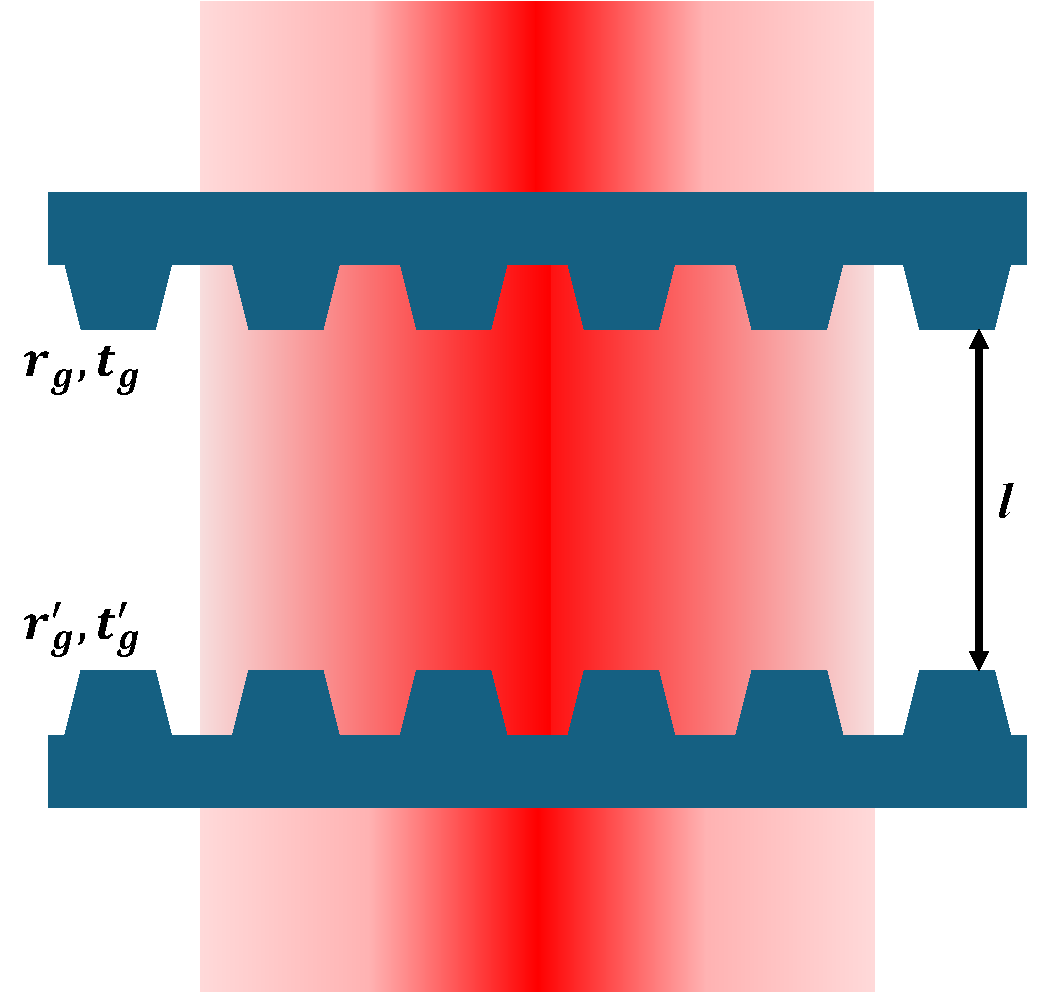
\includegraphics[width=\textwidth]{figures/double_fano_sketch.pdf}
        \caption{}
        \label{fig:double_fano_sketch}
    \end{subfigure}
    \caption{(a) shows schematics of the single Fano cavity consisting of a broadband mirror with transmission and reflectivity coefficients $t_m$, $r_m$ and a Fano mirror with coefficients $t_g$, $r_g$. (b) shows the schematics of the double Fano cavity consisting of two Fano mirrors with coefficients $t_g$, $r_g$, $t_g^{\prime}$, $r_g^{\prime}$. Both cavities are separated by a cavity length $l$.}
    \label{fig:single_and_double_fano_sketch}
\end{figure}

Here it is evident that instead of having one set of reflectivity and transmission coefficients that depend on the incident wavelength, we now have two. In order to model the transmission of the double Fano cavity, we once again consider the transmission function for the normal incident and planar Fabry-Perot cavity in eq. (\ref{eq:fabry_perot_trans}), this time with $r,t \rightarrow r_g(\lambda),t_g(\lambda)$ and $r^{\prime},t^{\prime} \rightarrow r_g^{\prime}(\lambda),t_g^{\prime}(\lambda)$\cite{Naesby}. We rewrite the Fabry-Perot transmission function with the addressed substitutions of the optical coefficients and such that it decribes the normalized transmission amplitudes $T_{cav} = |E_{out}|^2/|E_{0,in}|^2$ and get
\begin{equation}
    T_{cav} = \frac{t_g(\lambda) t_g^{\prime}(\lambda) e^{i\phi}}{1 - r_g(\lambda)r_g^{\prime}(\lambda) e^{2 i \phi}}.
    \label{eq:double_fano_transmission}
\end{equation}
The subscript $g$ indicates a grating transmission or reflectivity.

We now introduce a double Fano cavity consisting of two identical Fano mirrors, each as sketched in figure \ref{fig:MIST_grating_sketch} in section \ref{sec:fano_mirror}, and thus with optical parameters given in eq. (\ref{eq:optical_grating_params}). Figure \ref{fig:double_fano_transmission} shows an example of the normalized transmission spectrum of this double Fano cavity on- and off-resonance for a cavity length of $l \approx 30 \mu m$. The spectrum was found using eq. (\ref{eq:double_fano_transmission}).

\begin{figure}[h!]
    \centering
    \begin{subfigure}[c]{0.49\textwidth}
        \centering
        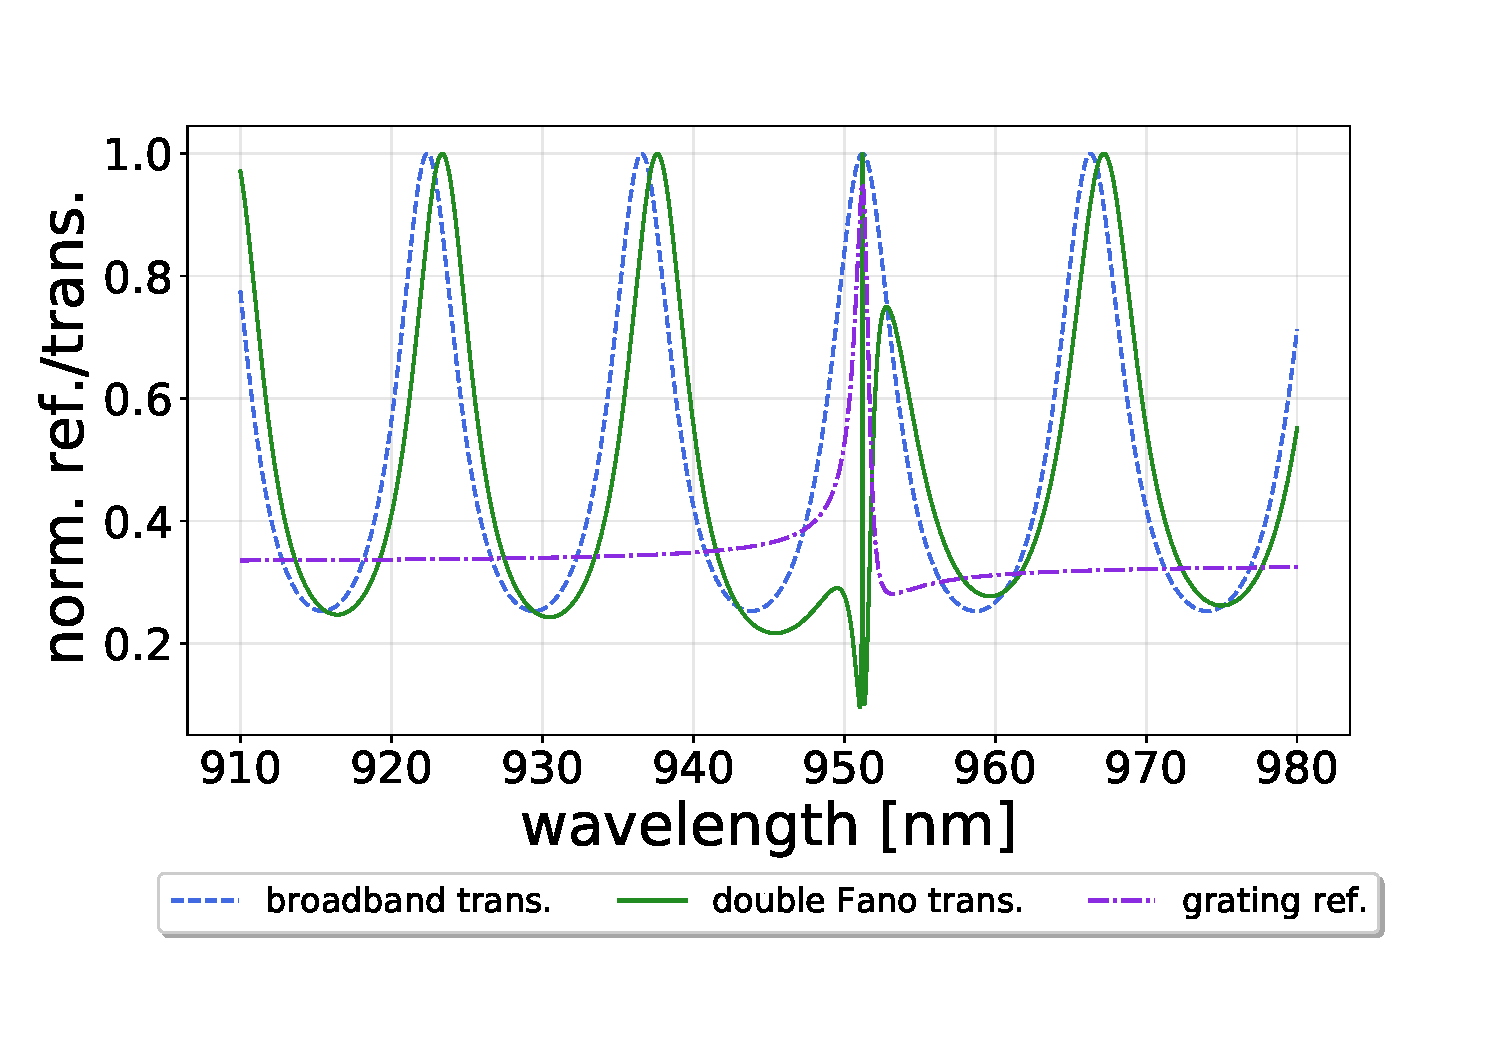
\includegraphics[width=\textwidth]{figures/double_fano_full_range_30um.pdf}
        \caption{}
        \label{fig:double_full_range}
    \end{subfigure}
    \begin{subfigure}[c]{0.49\textwidth}
        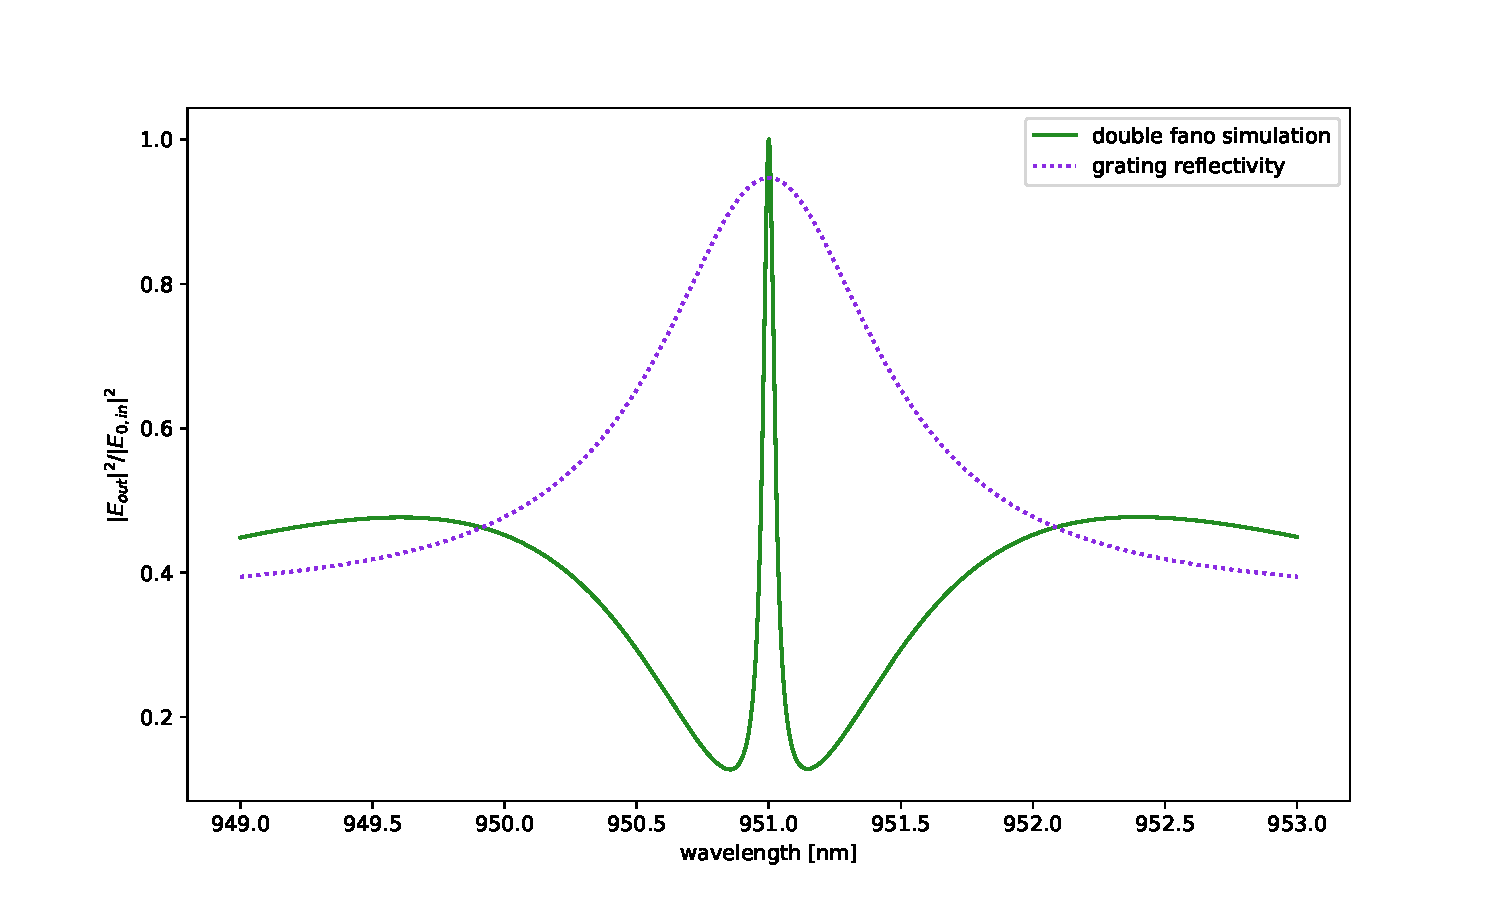
\includegraphics[width=\textwidth]{figures/double_fano_short_range_30um.pdf}
        \caption{}
        \label{fig:double_short_range}
    \end{subfigure}
    \caption{An example of a normalized double Fano transmission spectrum of a cavity of length $l \approx 30 \mu m$. (a) shows a long-range wavelength scan, depicting both the on- and off-resonance behaviour of the double Fano cavity transmission. Note that the broadband cavity transmission for a cavity of optical properties given by the direct reflectivity $r_d$ and direct transmission $t_d$ of the Fano mirror is shown. It is readily seen that the resonance peak is placed on a "background" consisting of this function, displaced by a small phase. (b) shows the transmission focussed specifically around the resonance wavelength. Both examples are shown together with the reflectivity of the Fano mirror used to model them.}
    \label{fig:double_fano_transmission}
\end{figure}

\subsubsection{Transmission linewidth}\label{sec:double_fano_lw_theory}

In order to describe the analytical linewidth of the transmisison profile of the double Fano cavity, we take a similar approach as in the single Fano case outlined in section \ref{sec:single_fano_cavity_trans_linewidth}. It can be shown from eq. (\ref{eq:analytical_linewidth}) when including the wavelength dependence of the optical coefficients of both Fano mirrors, that the HWHM $\delta \lambda$ of the double Fano cavity transmission profile is approximately given as
\begin{equation}
    \delta \lambda^{double} \approx \frac{1}{\frac{1}{\delta \lambda_c} + \frac{1}{\delta \lambda_g^{double}}},
    \label{eq:analytical_linewidth_double}
\end{equation}
where 
\begin{equation}
    \delta \lambda_c = \frac{\lambda_0^2}{8 \pi l} (|t_g(\lambda_0)|^2 + |t_g^{\prime}(\lambda_0)|^2 + L)
\end{equation}
is still the HWHM of a broadband cavity and
\begin{equation}
    \delta \lambda_g^{double} = \frac{\gamma \lambda}{4 (1-r_d)}(|t_g(\lambda_0)|^2 + |t_g^{\prime}(\lambda_0)|^2 + L).
    \label{eq:double_fano_linewidth_contribution}
\end{equation}
is the HWHM of the double Fano cavity in the Fano regime. Note that $\delta \lambda^{double} = \delta \lambda^{single}/2$ for $l \rightarrow 0$ when eq. (\ref{eq:analytical_linewidth_double}) is predominantly given by eq. (\ref{eq:double_fano_linewidth_contribution}). In this brief evaluation of the estimated analytical linewidth of the double Fano transmission profile it is assumed that all defining parameters of the two Fano mirrors are identical, except for the cavity and guided-mode resonance wavelengths $\lambda_{0,1}$. Namely the following relevant parameters are assumed identical,
\begin{equation}
    r_d = r_d^{\prime} \: \text{ and } \: \gamma \lambda = \gamma \lambda^{\prime}.
\end{equation}
In this way any spectral detuning of the two Fano mirrors used to make a cavity is included in the analytical expression. The spectral detuning, and the effect hereof, will be further described in section \ref{sec:spectral_detuning}.

\subsubsection{Single and double Fano cavity comparison}\label{sec:single_vs_double_comparison_theory}

Using the analytical expression for the double Fano cavity transmission in eq. (\ref{eq:analytical_linewidth_double}) we are now in a position to compare the single and double Fano cavities. Note that we at this point only consider the ideal case of the double Fano cavity where additional cavity losses are neglected and the two Fano mirrors used are identical, i.e. the cavity is said to be \emph{symmetrical}. The additional cavity losses are explicitly set to be given as
\begin{equation}
    L = 1-|r_g|^2-|t_g|^2 = 0.
\end{equation}

\begin{figure}[h!]
    \centering
    \begin{subfigure}[c]{0.49\textwidth}
        \centering
        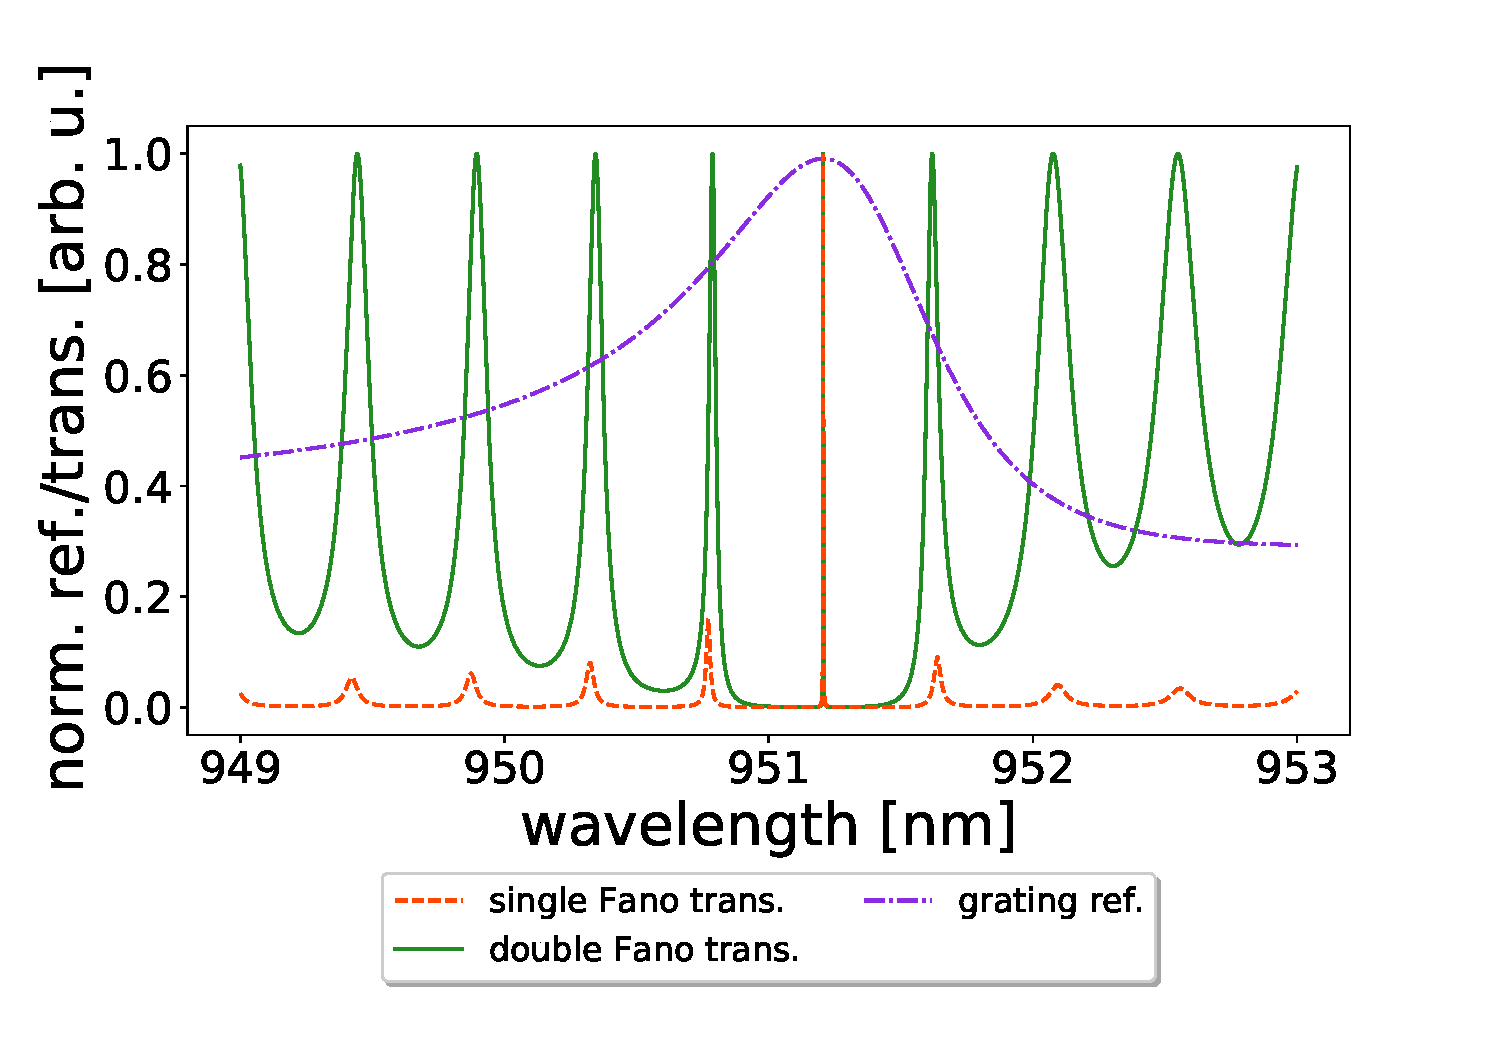
\includegraphics[width=\textwidth]{figures/single_and_double_1000um.pdf}
        \caption{}
        \label{fig:double_in_standard_regime}
    \end{subfigure}
    \begin{subfigure}[c]{0.49\textwidth}
        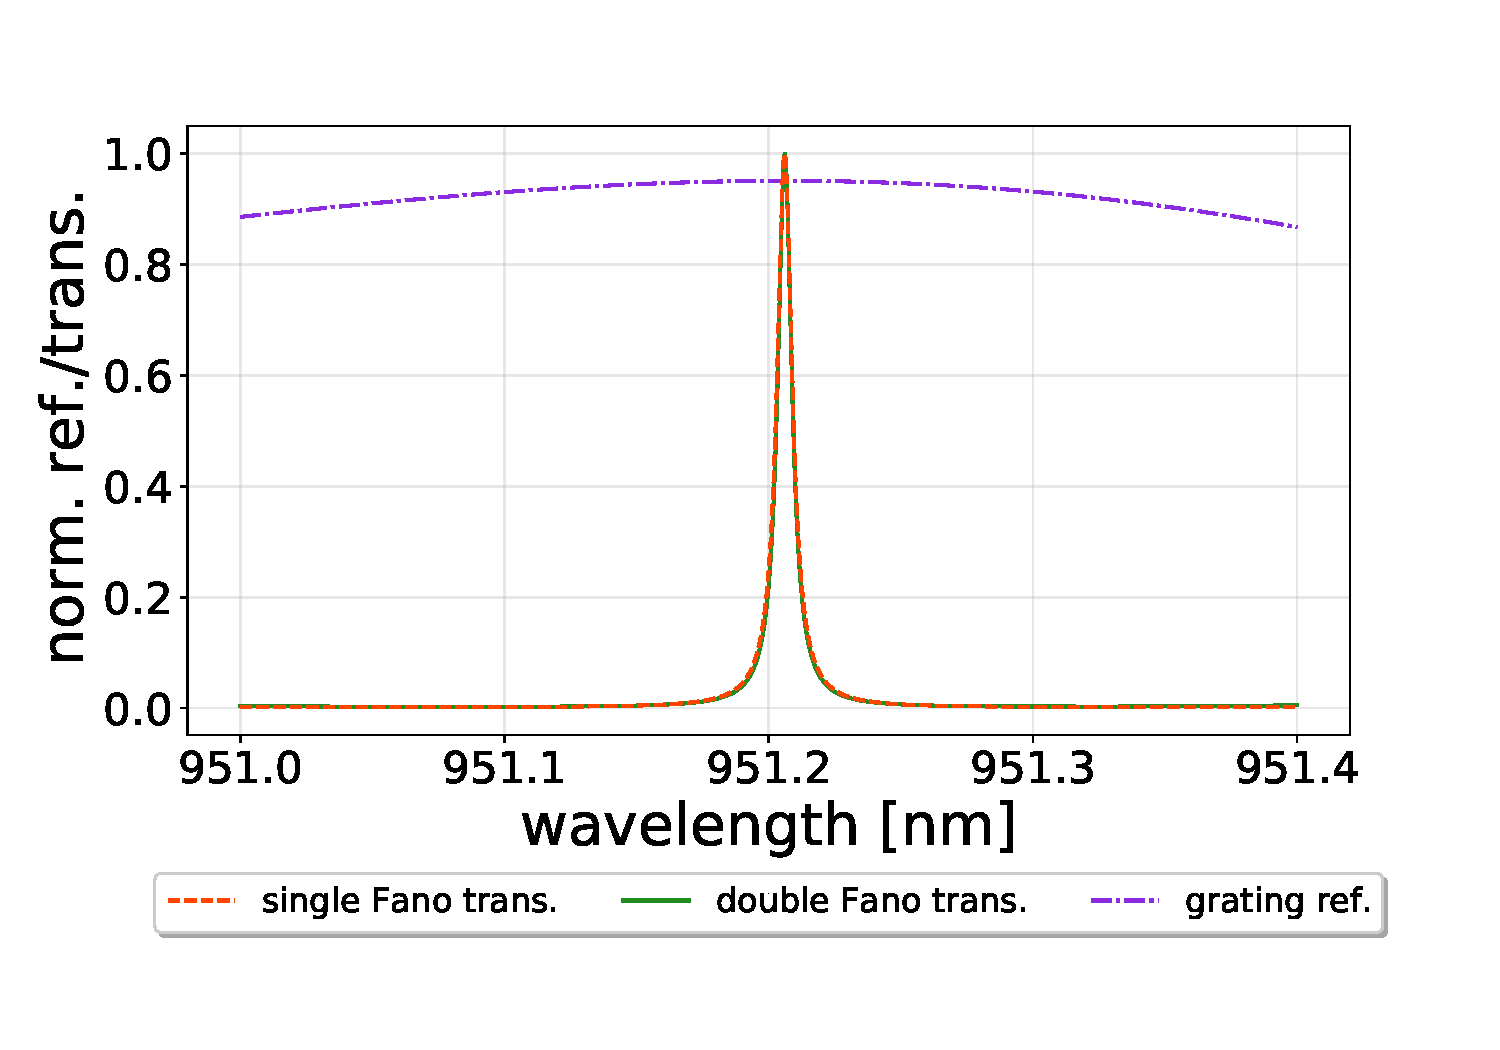
\includegraphics[width=\textwidth]{figures/single_and_double_1000um_zoomed.pdf}
        \caption{}
        \label{fig:double_in_standard_regime_zoomed}
    \end{subfigure}
    \begin{subfigure}[c]{0.49\textwidth}
        \centering
        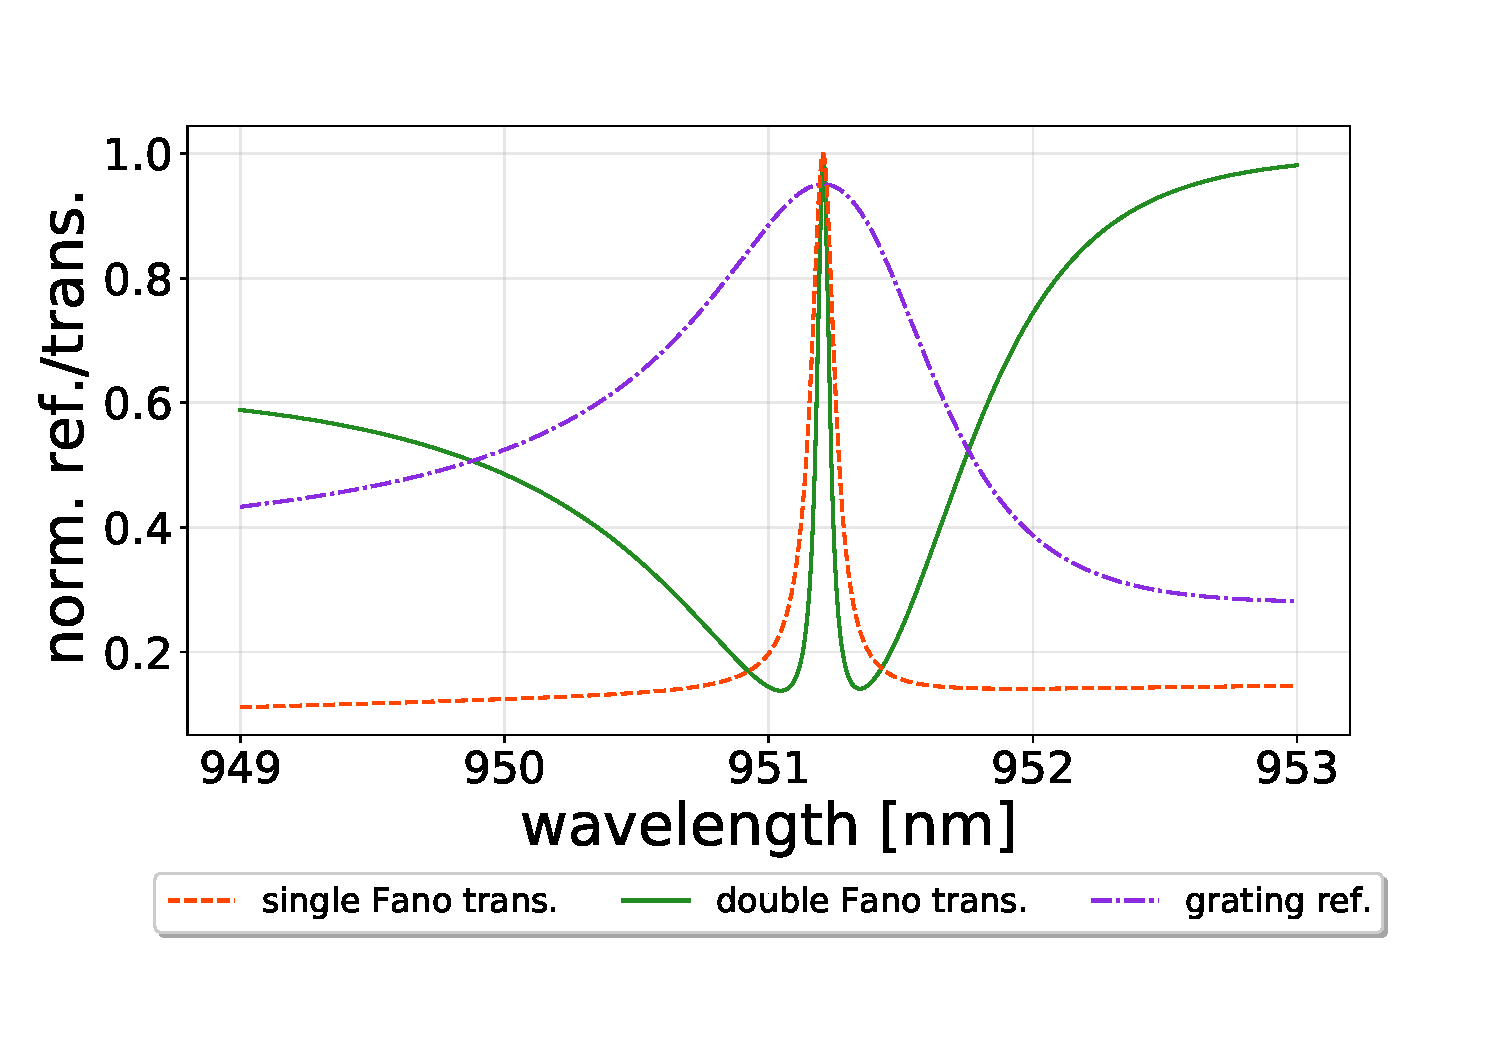
\includegraphics[width=\textwidth]{figures/single_and_double_5um.pdf}
        \caption{}
        \label{fig:double_in_fano_regime}
    \end{subfigure}
    \begin{subfigure}[c]{0.49\textwidth}
        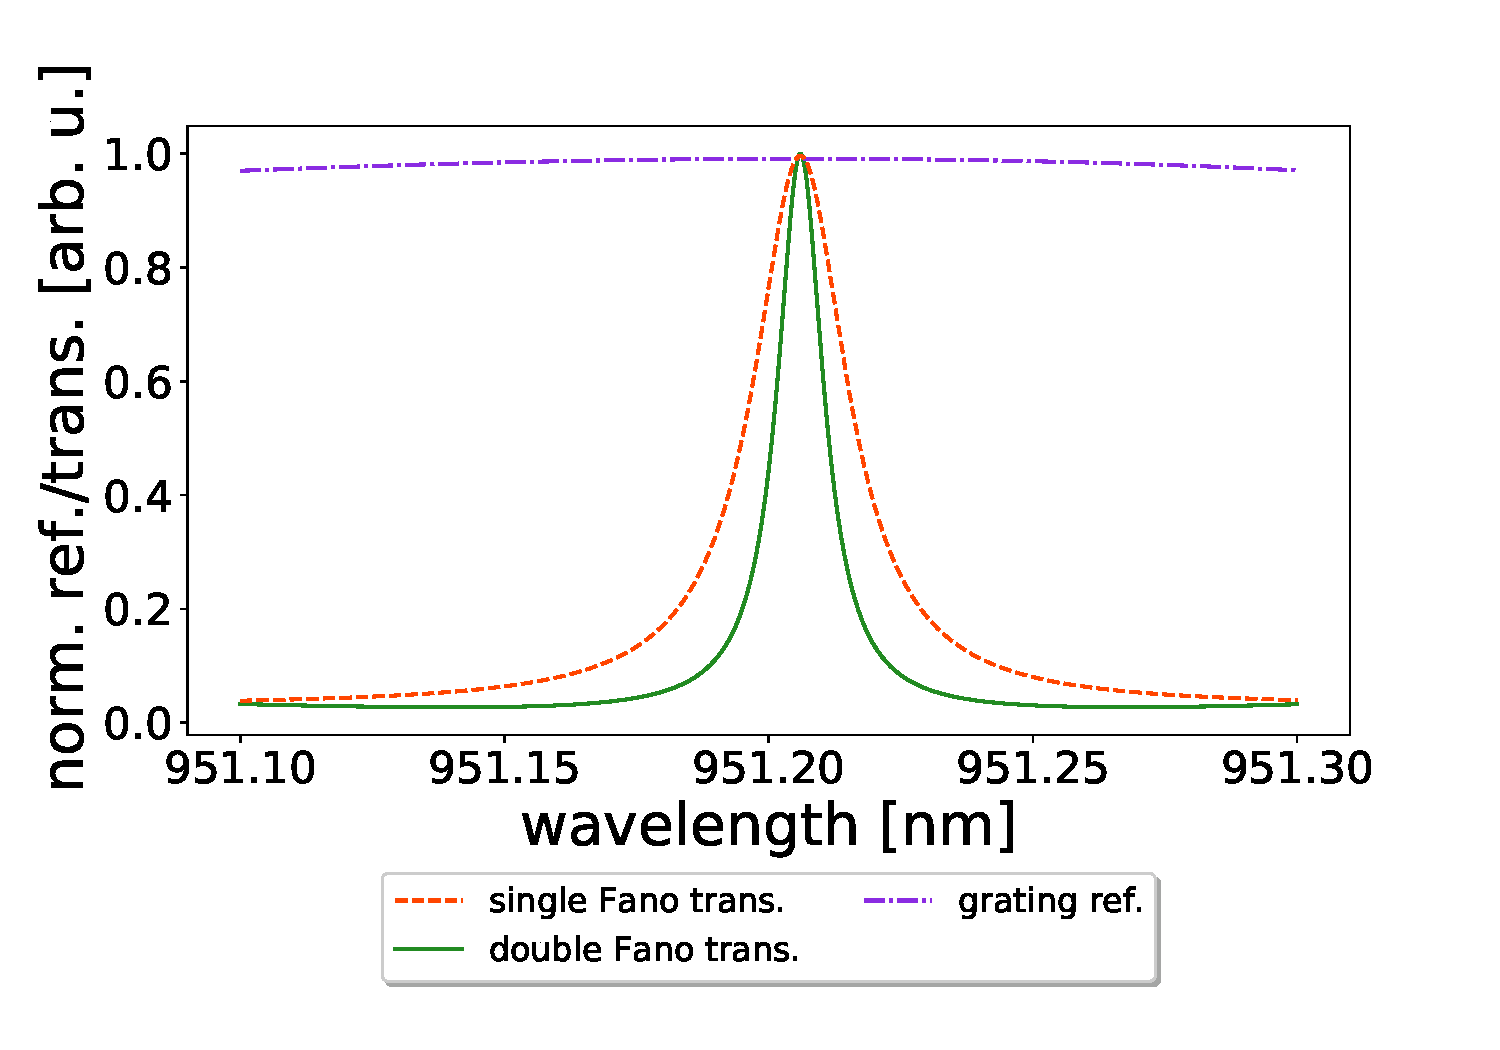
\includegraphics[width=\textwidth]{figures/single_and_double_5um_zoomed.pdf}
        \caption{}
        \label{fig:double_in_fano_regime_zoomed}
    \end{subfigure}
    \caption{Comparison of the single and double Fano transmission spectra in the \emph{standard} and \emph{Fano} regimes. (a) and (b) shows the spectral comparison for a cavity of length $l \approx 1000 \mu m$, i.e. in the \emph{standard} regime, while (c) and (d) shows the same for a cavity of length $l \approx 5 \mu m$, i.e. in the \emph{Fano} regime. (b) and (c) show spectra zoomed around the resonance peak, and the Fano mirror reflectivity is depicted in all figures.}
    \label{fig:double_in_standard_and_fano_regimes}
\end{figure}

Figure \ref{fig:double_in_standard_and_fano_regimes} shows the transmission of the ideal double Fano cavity and the corresponding single Fano cavity for comparison. 

Figures \ref{fig:double_in_standard_regime} and \ref{fig:double_in_standard_regime_zoomed} shows the transmission for a cavity length of $l \approx 1000 \mu m$ which is well-inside the standard regime outlined in section \ref{sec:single_fano_cavity_trans_linewidth}, where the standard, broadband and single Fano cavities produce transmission spectra of roughly identical linewidths. In this regime, due to the $1/l$ proportionality of the FSR, the off-resonance behavior of the double Fano cavity transmission is visible in the range plottet. It is seen, contrary to the single Fano cavity, that the transmission at each cavity resonance reaches a normalized transmission of $|E_{out}|^2/|E_{0,in}|^2=1$. This is due to the fact that the two Fano mirrors, while they have wavelength dependent transmission and reflectivity coefficients, always have identical ones for the ideal case. This maximizes the Fabry-Perot transmission function and ensures unity transmission at any cavity resonance. The minimum level of the cavity changes according to the coefficient of finesse, and thus only the Fano mirror reflectivity, hence the HWHM also changes as we move further from the guided-mode resonance. Both the minimum transmission level and the HWHM converge when moving away from the resonance wavelength, when $r \rightarrow r_d$ becomes constant. 

Figures \ref{fig:double_in_fano_regime} and \ref{fig:double_in_fano_regime_zoomed} shows the transmission of a double Fano cavity of length $l \approx 5 \mu m$, i.e. well within the Fano regime. It is seen that the double Fano cavity transmission produces a resonance peak with a HWHM narrower than the one for the single Fano cavity, as is predicted in eq. (\ref{eq:double_fano_linewidth_contribution}). Furthermore, the immediate off-resonance behavior of the double Fano cavity transmission in the Fano regime, is drastically different than for the single Fano cavity. This is due to the collective higher transmission in this region compared with the single Fano case where the broadband mirror has a constant, and often high, reflectivity and hence a correspondingly low transmission.

\begin{figure}[h!]
    \centering
    \begin{subfigure}[c]{0.7\textwidth}
        \centering
        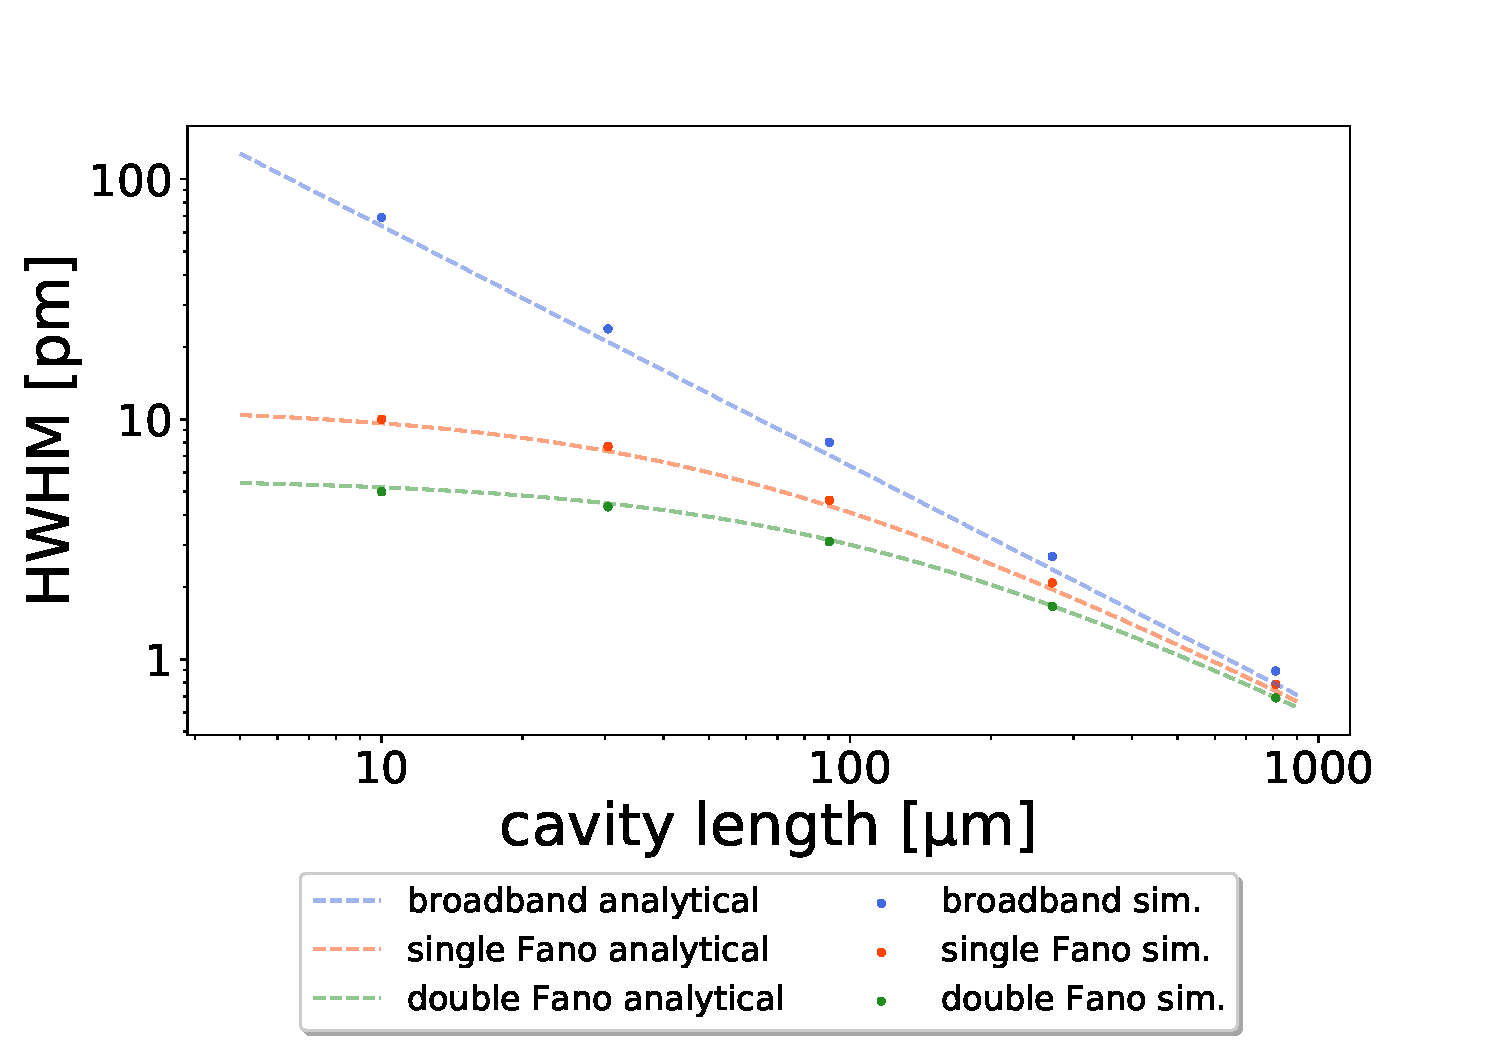
\includegraphics[width=\textwidth]{figures/HWHM_broadband_vs_single_vs_double_sim.pdf}
        \caption{}
        \label{fig:HWHM_double_vs_single_vs_broadband}
    \end{subfigure}
    \begin{subfigure}[c]{0.49\textwidth}
        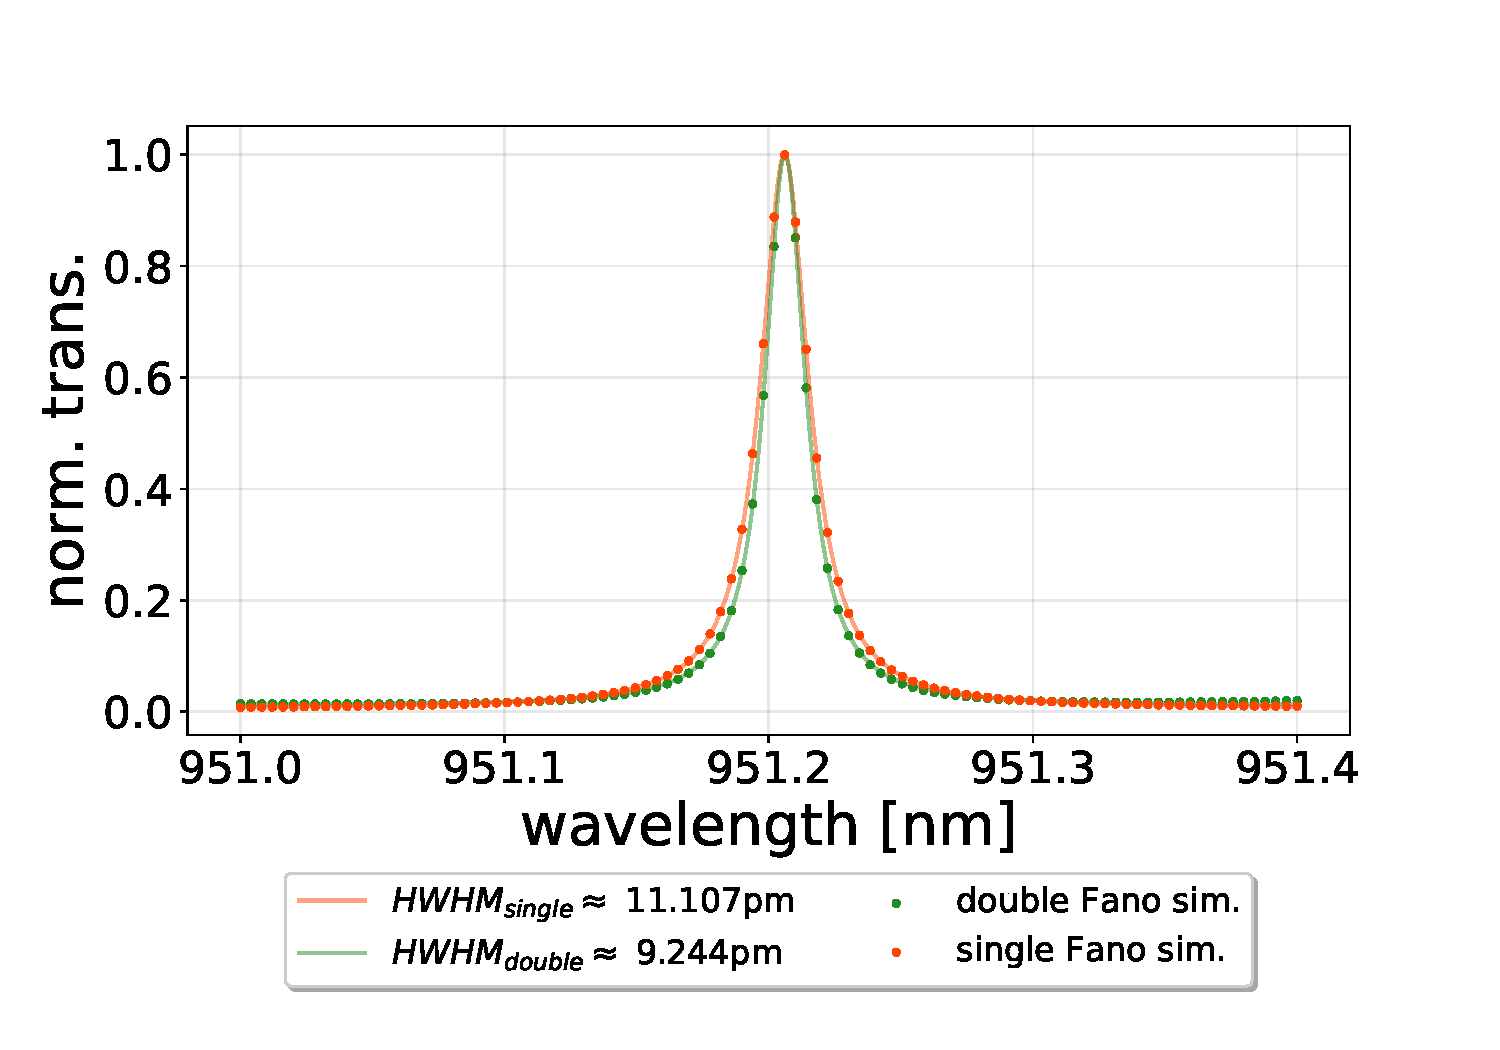
\includegraphics[width=\textwidth]{figures/sim_single_vs_double_270um.pdf}
        \caption{}
        \label{fig:700um_double_and_single_fano_peak}
    \end{subfigure}
    \begin{subfigure}[c]{0.49\textwidth}
        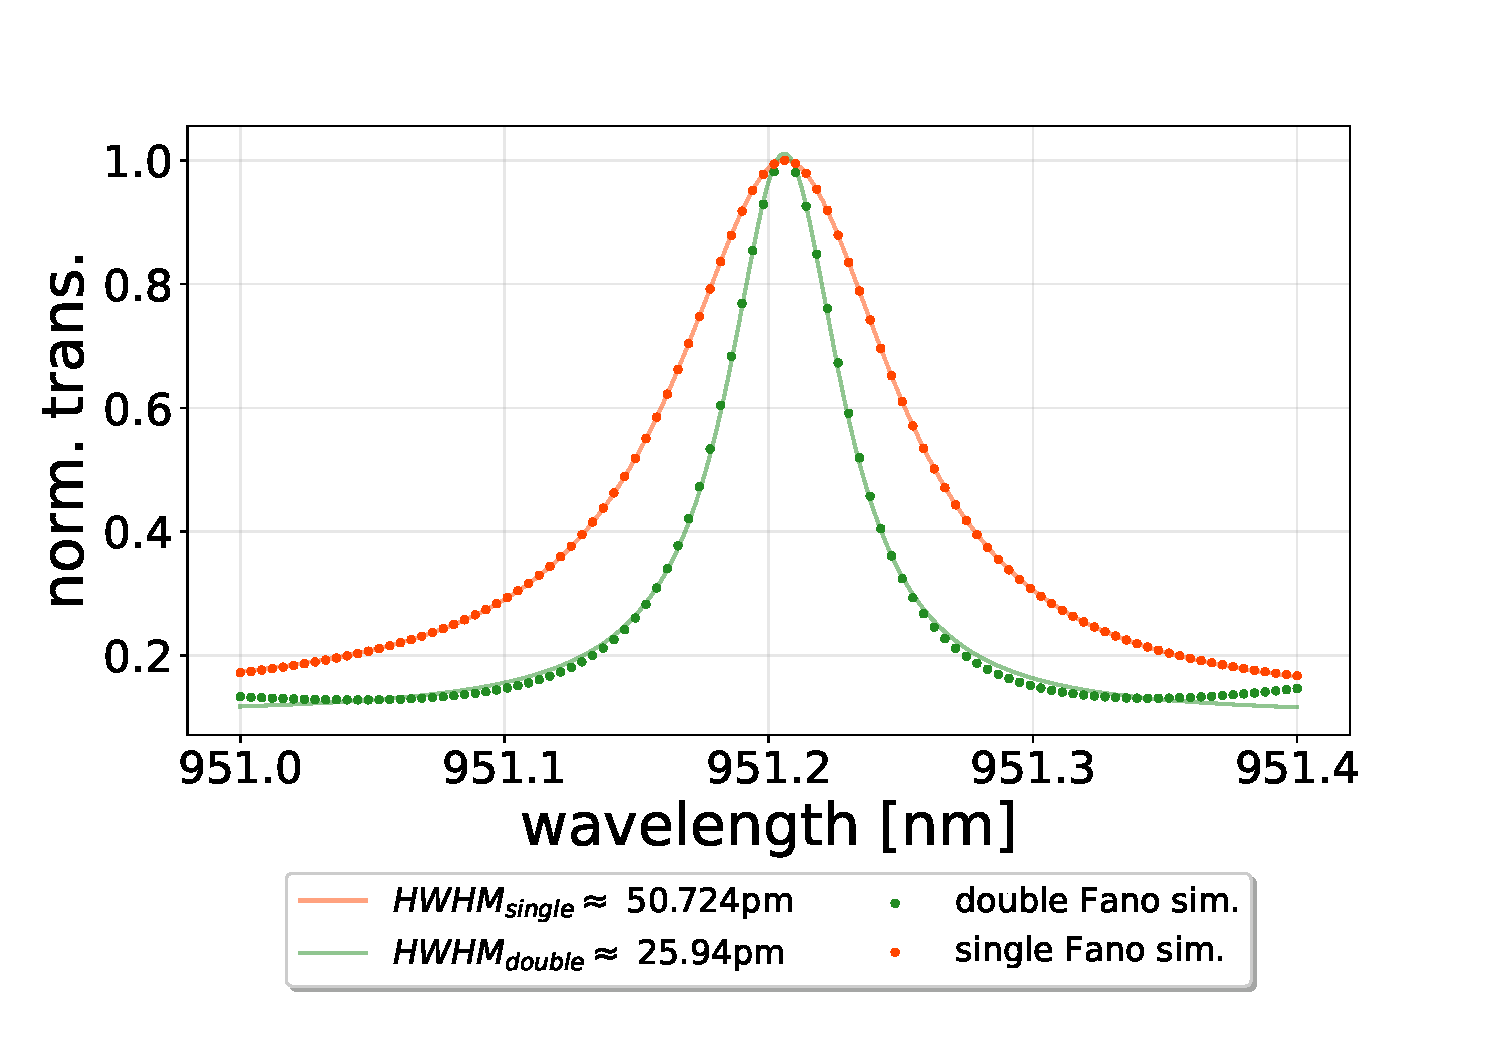
\includegraphics[width=\textwidth]{figures/sim_single_vs_double_10um.pdf}
        \caption{}
        \label{fig:10um_double_and_single_fano_peak}
    \end{subfigure}
    \caption{(a) shows the analytical resonance linewidths (eqs. (\ref{eq:analytical_linewidth}), (\ref{eq:analytical_linewidth_double}), and (\ref{eq:analytical_linewidth_broadband})) as a function of the cavity length for the broadband, single and double Fano cavities together with linewidths of corresponding profiles simulated using eqs. (\ref{eq:single_fano_trans}), (\ref{eq:double_fano_transmission}), and (\ref{eq:fabry_perot_trans}) for comparison. In (b) and (c) is seen transmission spectra of single and double Fano cavities of lengths $l \approx 270 \mu m$, and $l \approx 10 \mu m$, respectively. The spectra shown indicate each their respective linewidths, and are examples of the values plotted in (a). Note however, that the broadband cavity peak has been left out of (b) and (c).}
\end{figure}

Figure \ref{fig:HWHM_double_vs_single_vs_broadband} shows the analytical linewidth calculated and compared for the broadband, single Fano, and double Fano cavities, calculated using eqs. (\ref{eq:analytical_linewidth_broadband}), (\ref{eq:analytical_linewidth}), (\ref{eq:analytical_linewidth_double}). These are compared with linewidths found as fitting parameters from a least squares fit of the general Fano transmission formula given in eq. (\ref{eq:general_fano_model}) to transmission spectra calculated using eqs. (\ref{eq:fabry_perot_trans}), (\ref{eq:single_fano_trans}), and (\ref{eq:double_fano_transmission}). According to eq. (\ref{eq:analytical_linewidth_double}) the linewidth of the double Fano cavity transmission should converge to exactly half that of the single Fano cavity, meaning that
\begin{equation}
    \delta \lambda_{double} = \frac{\delta \lambda_{single}}{2}, \hspace{0.5cm} \text{for } l \rightarrow 0.
\end{equation}
This is supported well by the simulation depicted in figure \ref{fig:HWHM_double_vs_single_vs_broadband}.

Figures \ref{fig:700um_double_and_single_fano_peak} and \ref{fig:10um_double_and_single_fano_peak} contain examples of transmission spectra of single- and double Fano cavities and corresponding least squares fits to the general Fano model in order to determine their linewidths. 

\subsubsection{Additional cavity losses}\label{sec:additional_losses_theory}

Thus far we have only examined a lossless double Fano cavity where
\begin{equation}
    |r_g|^2 + |t_g|^2 = 1
\end{equation}
is fulfilled for both Fano mirrors used to contruct the cavity.

\begin{figure}[h!]
    \centering
    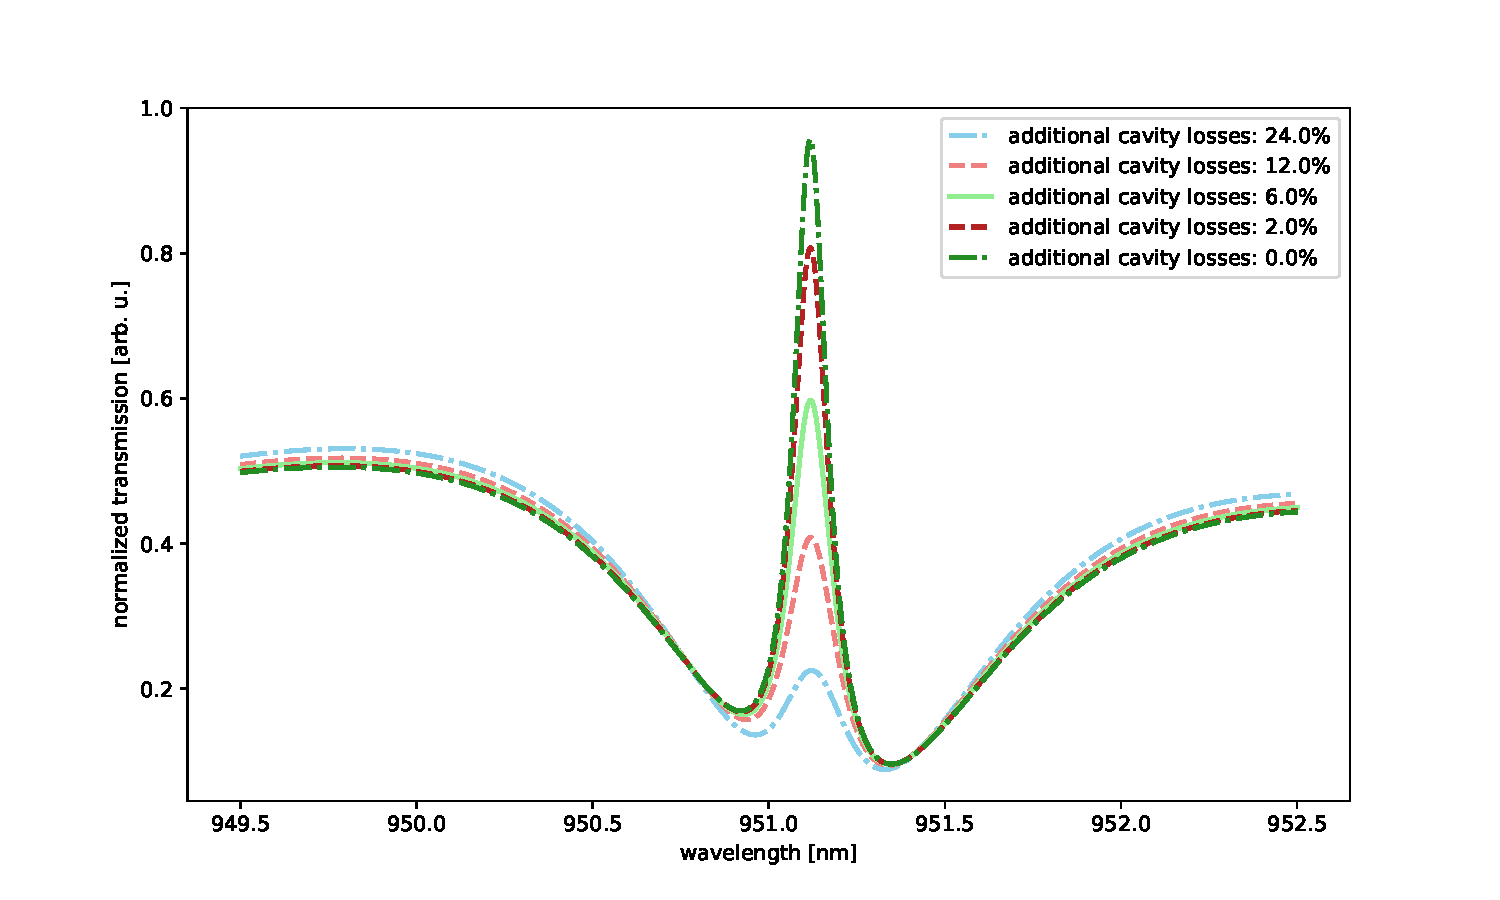
\includegraphics[width=0.6\textwidth]{figures/double_fano_loss_scan.pdf}
    \caption{Resonant transmission spectra for different values of the additional resonant loss term $L$, of a symmetric double Fano cavity of length $l \approx 30 \mu m$.}
    \label{fig:double_loss_scan}
\end{figure}

In this section we will investigate what happens when we introduce \emph{additional} cavity losses, not to be confused with the often used definition of cavity losses defined as $L=1-|r|^2$ where anything not being reflected back into the cavity is considered as "losses". Additional cavity losses, as described in this section, is given as
\begin{equation}
    L = 1 - |r_g|^2 - |t_g|^2,
\end{equation}
leading to the modified conervation condition
\begin{equation}
    |r_g|^2 + |t_g|^2 + L = 1.
\end{equation}

Figure \ref{fig:double_loss_scan} shows double Fano transmission spectra for a symmetric cavity with varying values for the additional cavity losses. It is readily seen that the maximum value reached in each spectrum is rapidly reduced with the introduction of these losses. 

Since the linewidth is defined as the HWHM of the transmission profile, this will naturally vary as a function of additional cavity losses. This is depicted in figure \ref{fig:HWHM_vs_losses} where the HWHM is shown for different values of $L$. Examples of transmission spectra taken for different values of $L$ are shown in figures \ref{fig:lossy_spectrum_0.2percent} and \ref{fig:lossy_spectrum_3.2percent}, along with their respective least squares fits to the general Fano model in eq. (\ref{eq:general_fano_model}) and linewidths found as fitting parameters hereof. 

\begin{figure}[h!]
    \centering
    \begin{subfigure}[c]{0.7\textwidth}
        \centering
        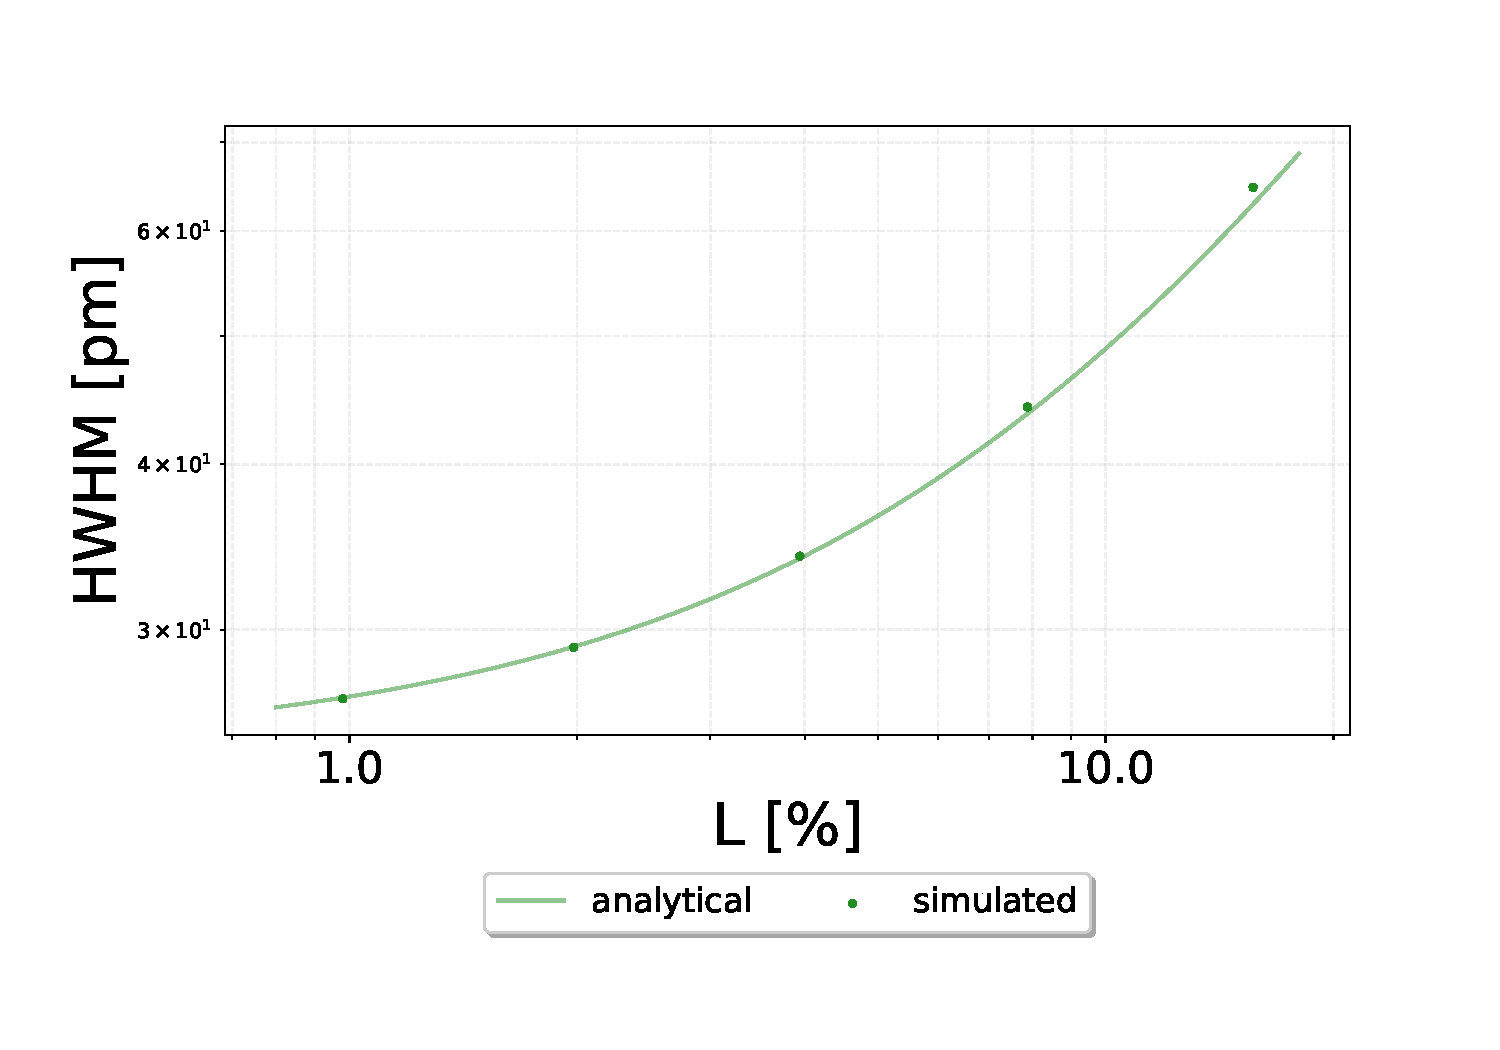
\includegraphics[width=\textwidth]{figures/linewidth_vs_losses.pdf}
        \caption{}
        \label{fig:HWHM_vs_losses}
    \end{subfigure}
    \begin{subfigure}[c]{0.49\textwidth}
        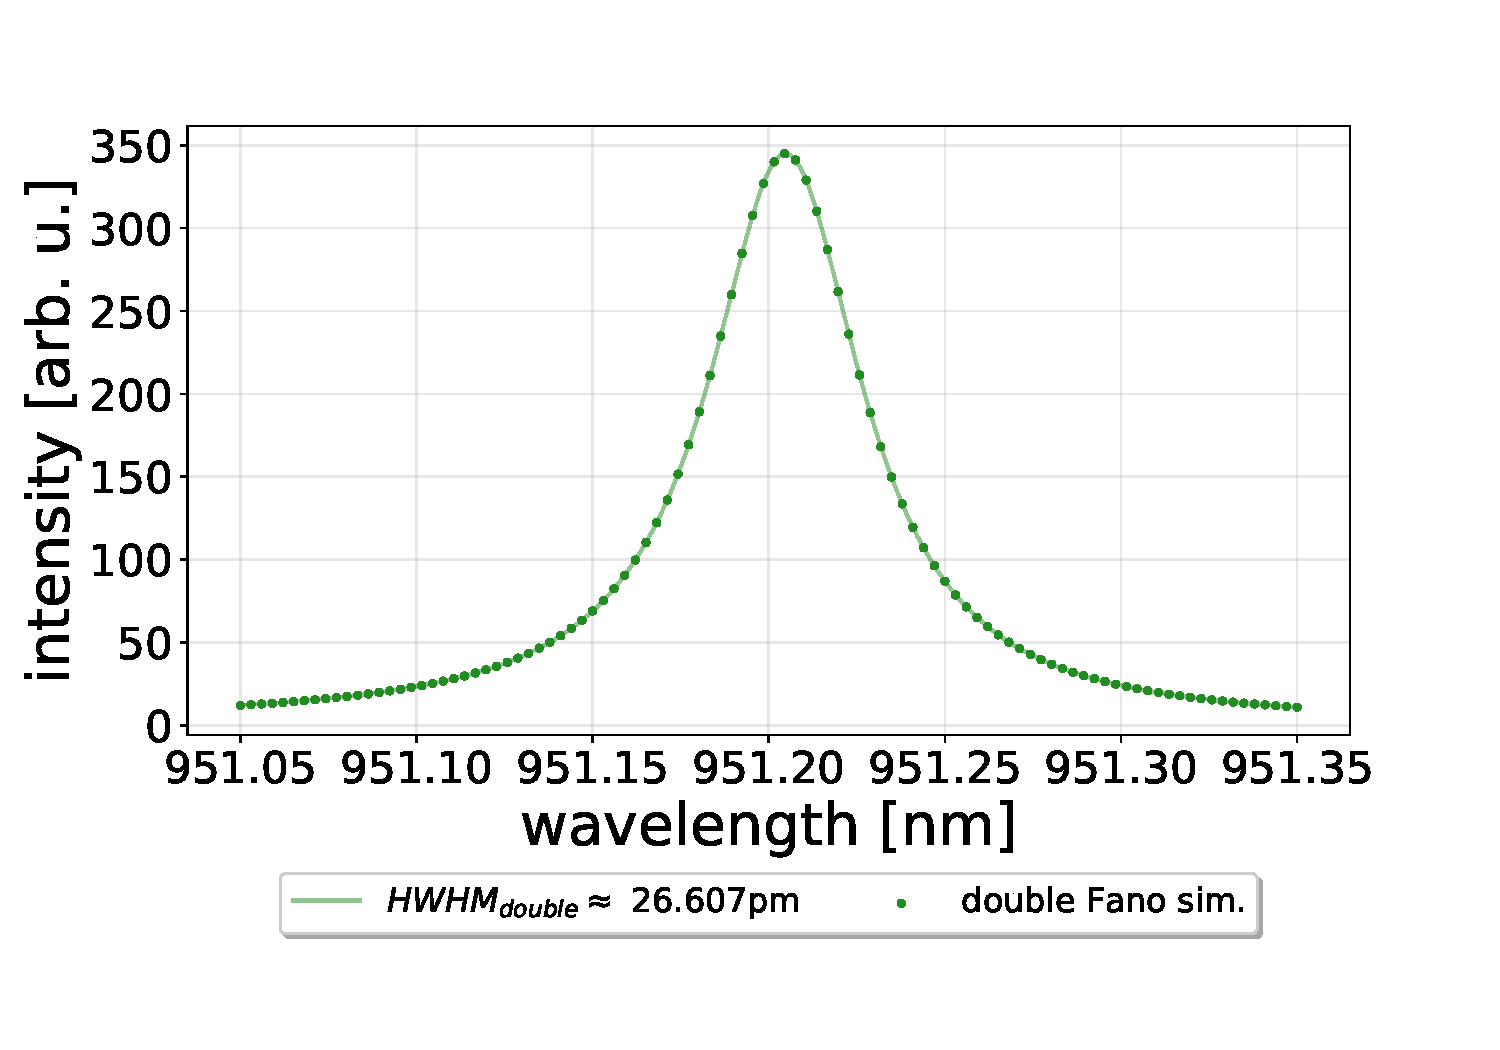
\includegraphics[width=\textwidth]{figures/double_1percent_loss_30um.pdf}
        \caption{}
        \label{fig:lossy_spectrum_0.2percent}
    \end{subfigure}
    \begin{subfigure}[c]{0.49\textwidth}
        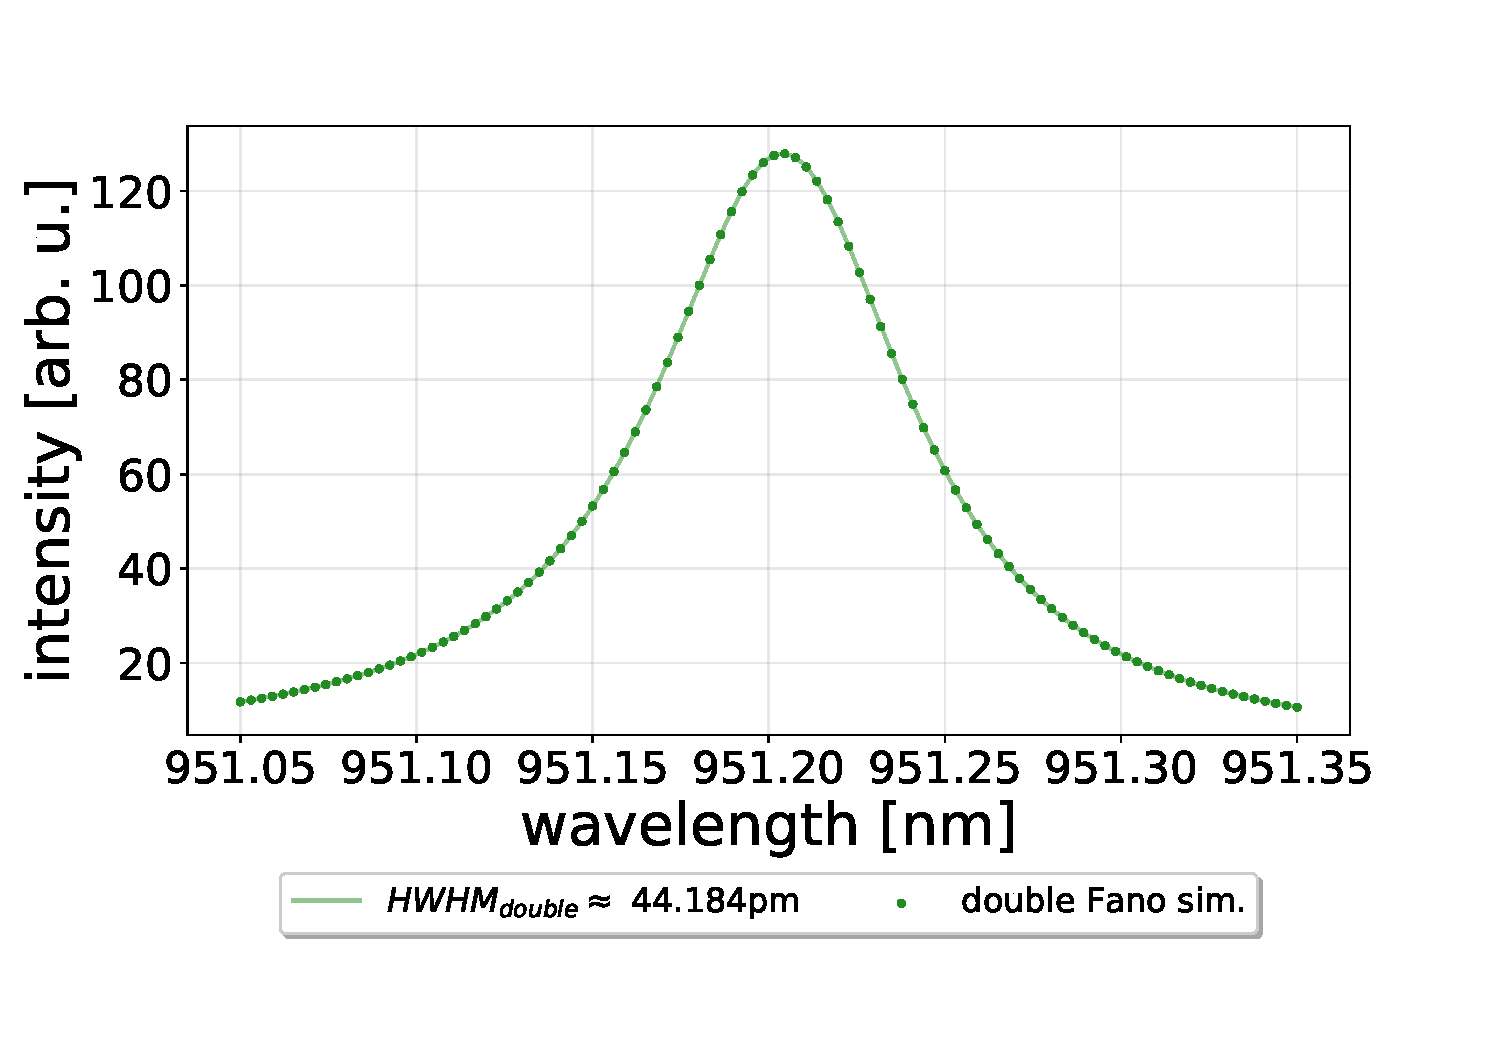
\includegraphics[width=\textwidth]{figures/double_8percent_loss_30um.pdf}
        \caption{}
        \label{fig:lossy_spectrum_3.2percent}
    \end{subfigure}
    \caption{(a) shows the linewidth (HWHM) of a symmetric double Fano cavity of length $l \approx 30 \mu m$  as a function of additional cavity losses $L = 2(1 - |r_g|^2 - |t_g|^2)$. Each point is found as a fitting parameter of a least squares fit of the double Fano intracavity spectrum for a certain value of $L$ to the general Fano model. The plotted line indicates the analytical value of the linewidth (eq. \ref{eq:analytical_linewidth}) as a function of $L$, for comparison. In (b) and (c) are seen examples of double Fano transmission spectra, with their respective linewidths, for cavities of $L=1\%$ and $L=8\%$, respectively.}
    \label{fig:HWHM_vs_losses_whole_figure}
\end{figure}

Figure \ref{fig:HWHM_vs_losses} shows the simulated linewidths of resonance transmission spectra as a function of the total additional cavity losses $L$, and is compared with the analytical formula for the double Fano linewidth in eq. (\ref{eq:analytical_linewidth_double}).

\subsubsection{Spectral detuning (lossless)} \label{sec:spectral_detuning}

Up until this point, it has been assumed that the Fano mirrors making up the double Fano cavity has been identical, namely the cavity has been \emph{symmetrical}. However, in practice this is very unlikely to be the case, as any Fano mirror constructed is bound to have some uncertainties attached to the physical parameters describing it (see eq. (\ref{eq:physical_grating_params})). For that reason we investigate the effect of an \emph{assymetric} cavity on the resulting transmission profile. Here we remember that each Fano mirror is describes by a set of parameters, $\lambda_0$, $\lambda_1$, $t_d$, $\gamma \lambda$ and $\beta$, which respectively describe the cavity resonance wavelength, guided-mode resonance wavelength, direct transmission, guided-mode resonance linewidth and additional losses of each grating. In order to model only a spectral detuning, we therefore simply change the parameters regarding the cavity and guided-mode resonance wavelengths, $\lambda_0$ and $\lambda_1$ by an amount corresponding to the detuning we wish to study. For this section the parameters will be given by the ones for the Fano mirror skecthed in figure \ref{fig:MIST_grating_sketch}, and thus given in eq. (\ref{eq:optical_grating_params}) for the unchanged Fano mirror, and
\begin{equation}
    \begin{split}
    \lambda_0^{\prime} = &\lambda_0 + \Delta,\:\: \lambda_1^{\prime} = \lambda_1 + \Delta,\:\: t_d^{\prime} = t_d,\\ &\gamma \lambda^{\prime} = \gamma \lambda\: \text{ and }\: \beta^{\prime} = \beta
    \end{split}
    \label{eq:detuned_grating_params}
\end{equation}
for the \emph{detuned} Fano mirror, where $\Delta$ is the detuning given by $\Delta = |\lambda_0 - \lambda_0^{\prime}|$. Figure \ref{fig:detuned_grating_spectra} shows the normalized reflectivity and transmission spectra of the unchanged Fano mirror (eq. (\ref{eq:optical_grating_params})) and the detunined Fano mirror (eq. (\ref{eq:detuned_grating_params})) for a detuning of $\Delta = 0.3$nm.

\begin{figure}[h!]
    \centering
    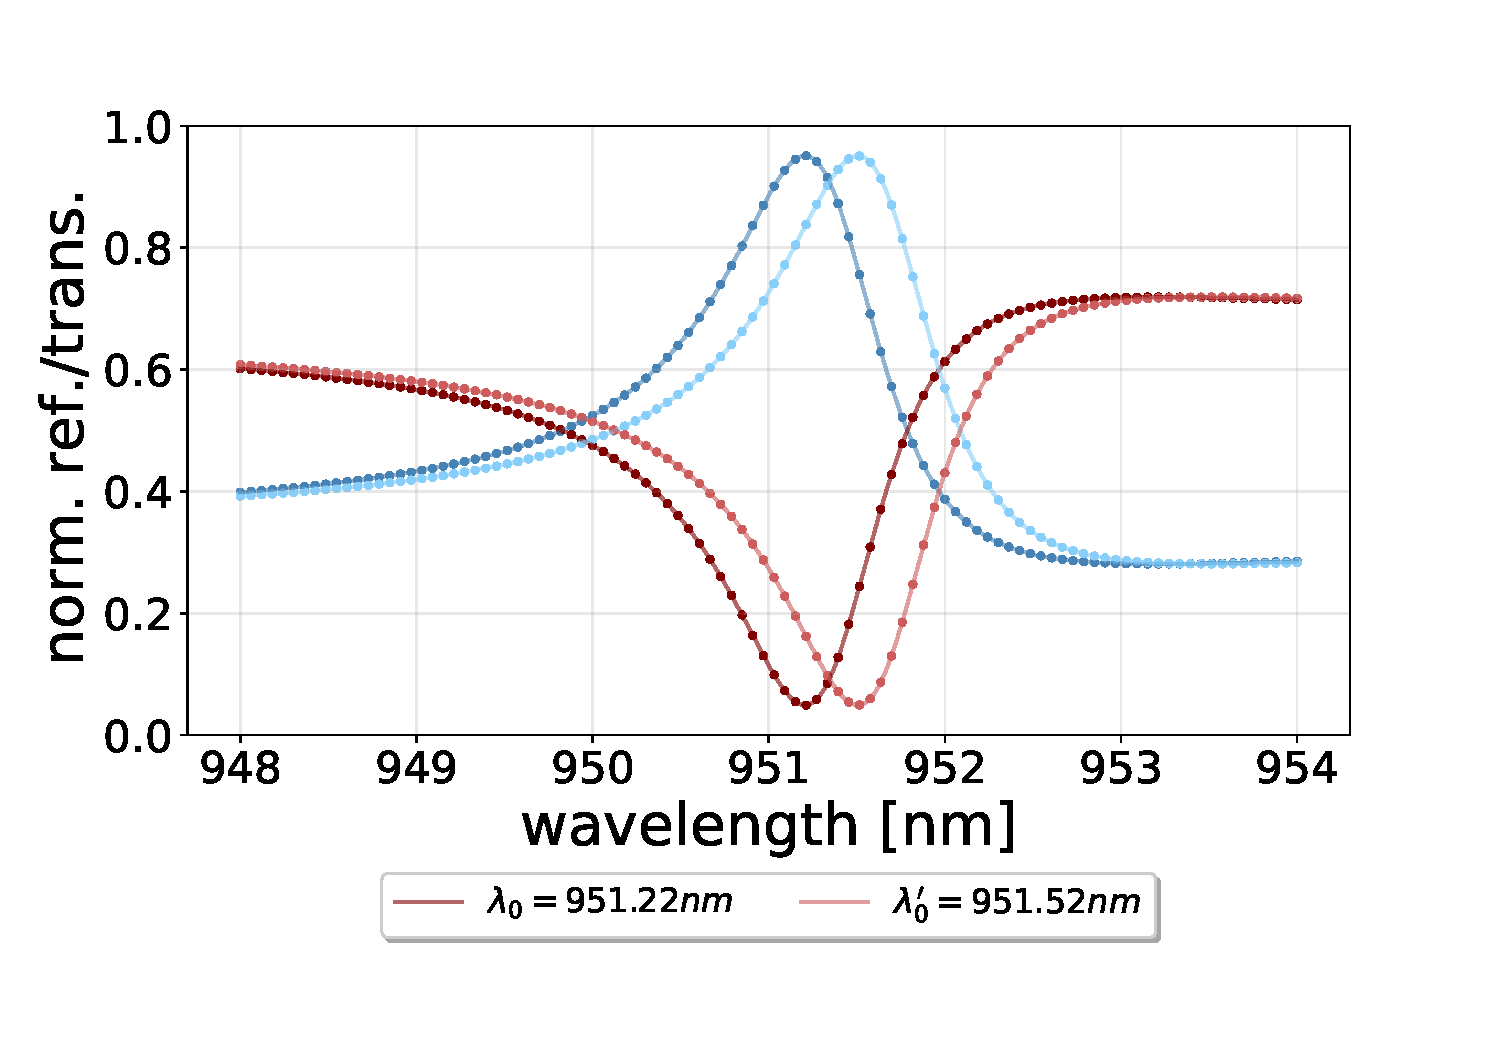
\includegraphics[width=0.7\textwidth]{figures/detuned_grating_spectra.pdf}
    \caption{The normalized reflectivity and transmission spectra of the Fano mirrors described in eqs. (\ref{eq:optical_grating_params}) and (\ref{eq:detuned_grating_params}) for detuning $\Delta = 0.3nm$.}
    \label{fig:detuned_grating_spectra}
\end{figure}

As has been observed in previous sections, the Fano resonance transmission peak is present at the point where the grating reflectivity $r_g(\lambda)$ is maximized and transmission $t_g(\lambda)$ minimized. However, when $\lambda_0 \neq \lambda_0^{\prime}$ and $\lambda_1 \neq \lambda_1^{\prime}$, this is no longer a trivial conclusion to draw. The question of whether the cavity resonance should be tuned to match the guided-mode resonance wavelength of one grating or the other, or maybe somewhere in between does not have an obvious answer. This will be further expanded upon later in section \ref{sec:spacial_detuning}, but in order to move forward with the investigation of the spectral detuning we, for now, accept that the optimal cavity length, is the one corresponding to a cavity resonance $\lambda_t$ given, exactly between the two guided-mode resonance wavelengths, as 
\begin{equation}
    \lambda_t = \frac{\lambda_{0} + \lambda_{0}^{\prime}}{2}.
    \label{eq:transmission_wavelength}
\end{equation}
Where \emph{t} is for \emph{transmission} as this is, later on, to be used experimentally as the \emph{transmission wavelength}. 

\begin{figure}[h!]
    \centering
    \begin{subfigure}[b]{0.49\textwidth}
        \centering
        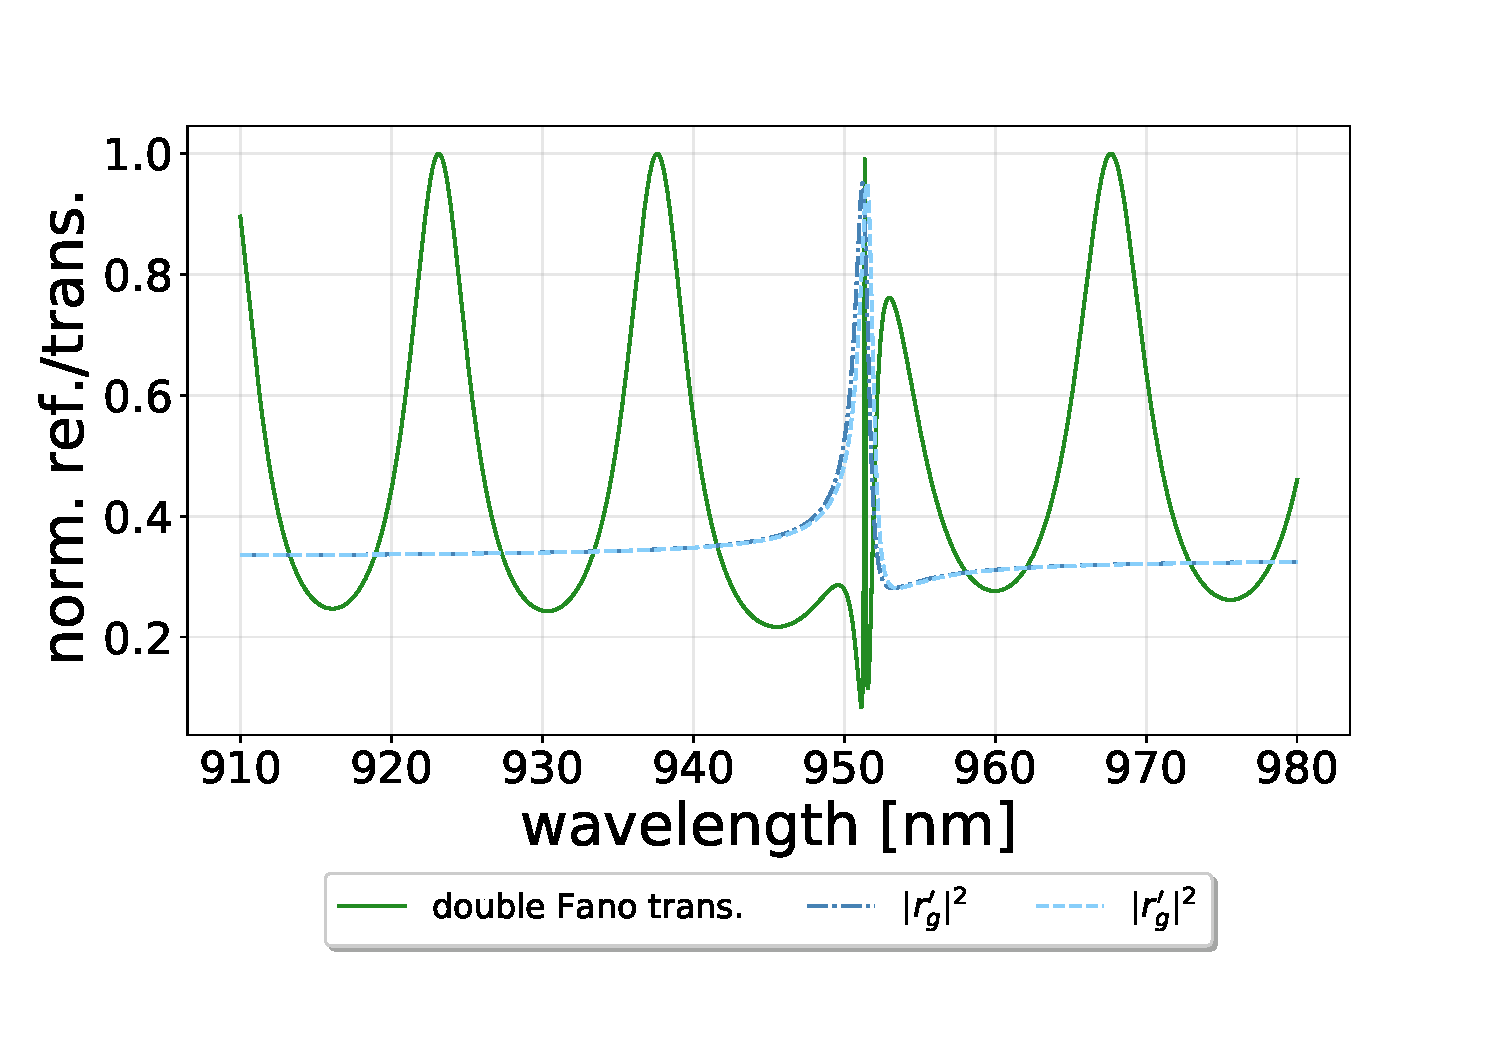
\includegraphics[width=\textwidth]{figures/detuned_full_range_double_trans.pdf}
        \caption{}
        \label{fig:full_range_detuned_trans}
    \end{subfigure}
    \begin{subfigure}[b]{0.49\textwidth}
        \centering
        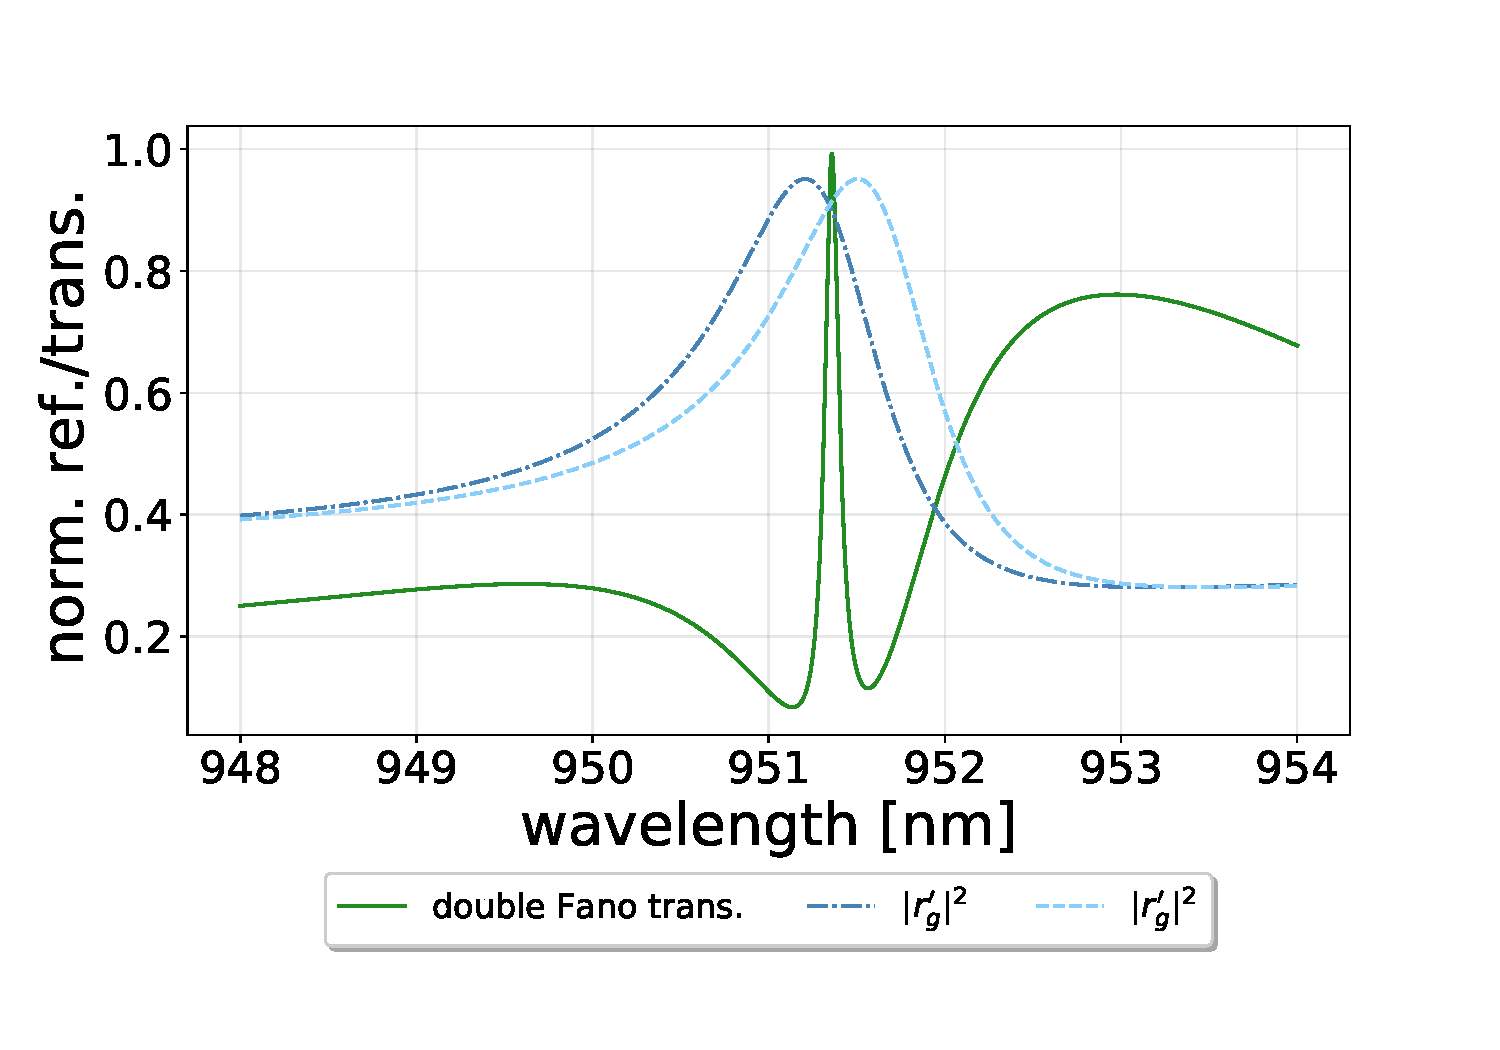
\includegraphics[width=\textwidth]{figures/detuned_short_range_double_trans.pdf}
        \caption{}
        \label{fig:short_range_detuned_trans}
    \end{subfigure}
    \caption{The double Fano transmission spectra of a cavity of length $l \approx 30 \mu m$ and detuned by $\Delta = 0.3$nm, as seen in figure \ref{fig:detuned_grating_spectra}, together with the reflectivity spectra of the Fano mirrors used for the simulation.}
    \label{fig:detuned_double_fano_transmission}
\end{figure}

Figure \ref{fig:detuned_double_fano_transmission} shows the transmission spectrum of a detuned double Fano cavity with parameters corresponding to the transmission and reflectivity spectra in figure \ref{fig:detuned_grating_spectra}, meaning that $\Delta = 0.3$nm. The transmission wavelength $\lambda_t$ is chosen such that eq. (\ref{eq:transmission_wavelength}) is fulfilled, and correspondingly it is seen that the transmission peak is placed exactly between the maximum (minimum) reflectivites (transmissions) of the two grating, i.e. between the two guided-mode resonance wavelengths. Furthermore, it can be concluded that the detuning is chosen such that the overlap between the guided-mode resonances is still substantiel enough for them to couple and hence for the overall Fano resonance to be excited. 

While knowing that a detuning of $0.3$nm is acceptable in terms of exciting the Fano resonance in the lossless case is a nice result, it does not provide much in terms of estimating the acceptable detuning for any experimental purposes. In figure \ref{fig:detuning_scan} the double Fano transmission is shown for increasing detuning $\Delta$ and transmission wavelength $\lambda_t = (\lambda_{0} + \lambda_{0}^{\prime}(\Delta))/2$. 

\begin{figure}[h!]
    \centering
    \begin{subfigure}[b]{0.49\textwidth}
        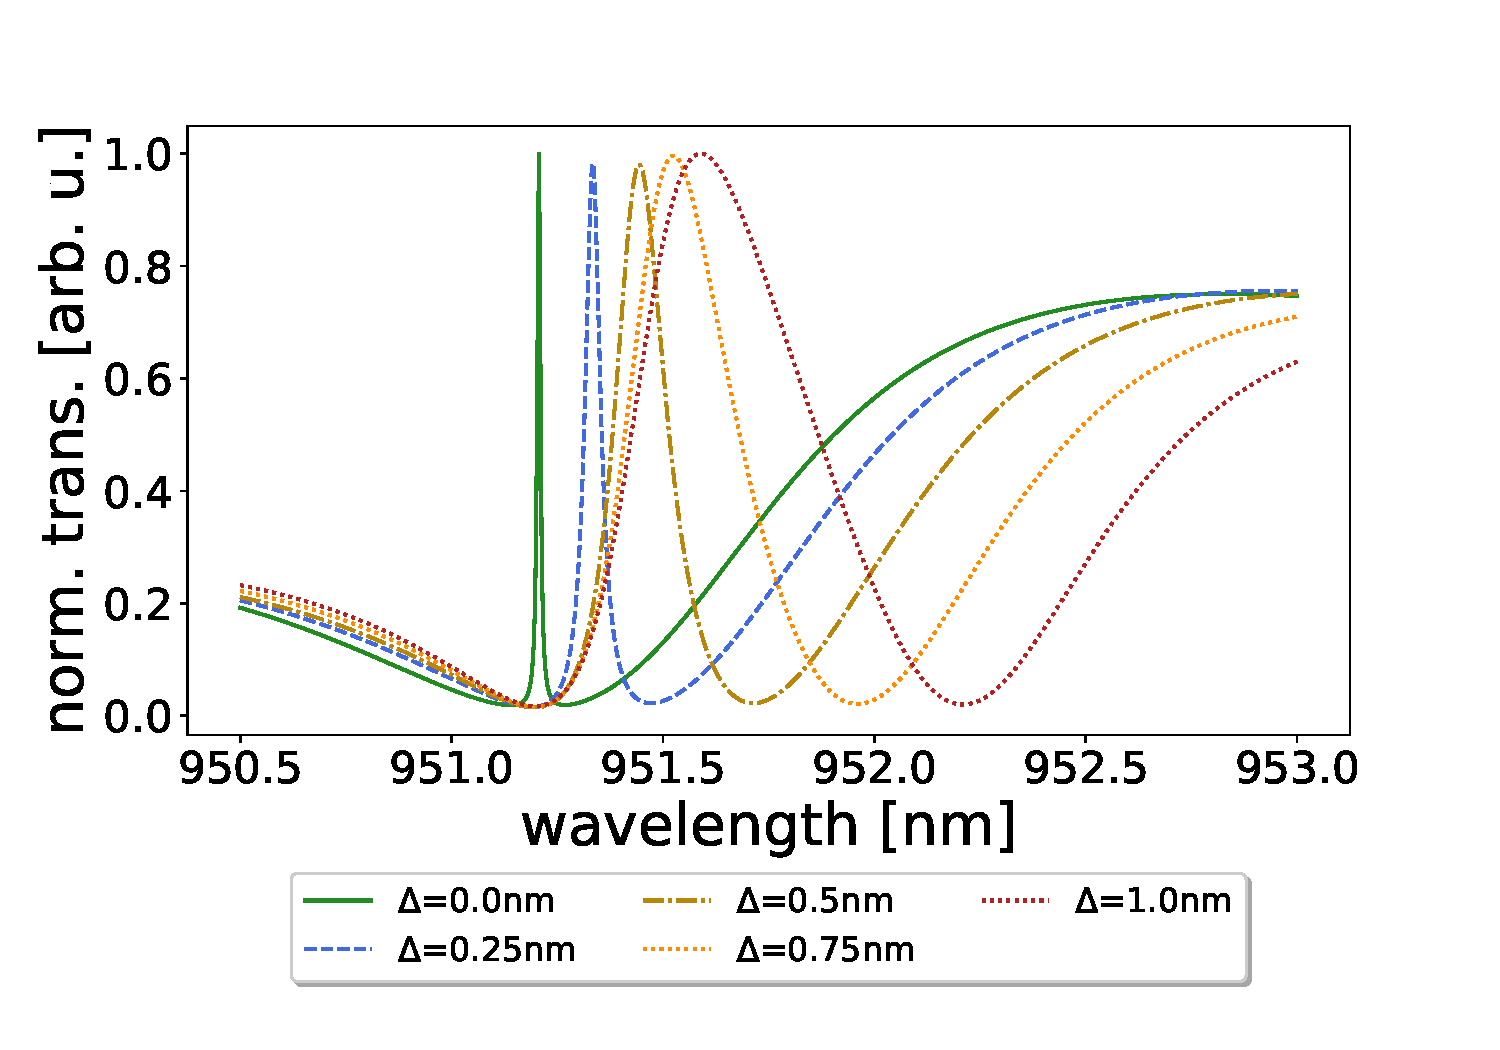
\includegraphics[width=\textwidth]{figures/detuning_scan_double_fano_30um.pdf}
        \caption{}
        \label{fig:detuning_scan}
    \end{subfigure}
    \begin{subfigure}[b]{0.49\textwidth}
        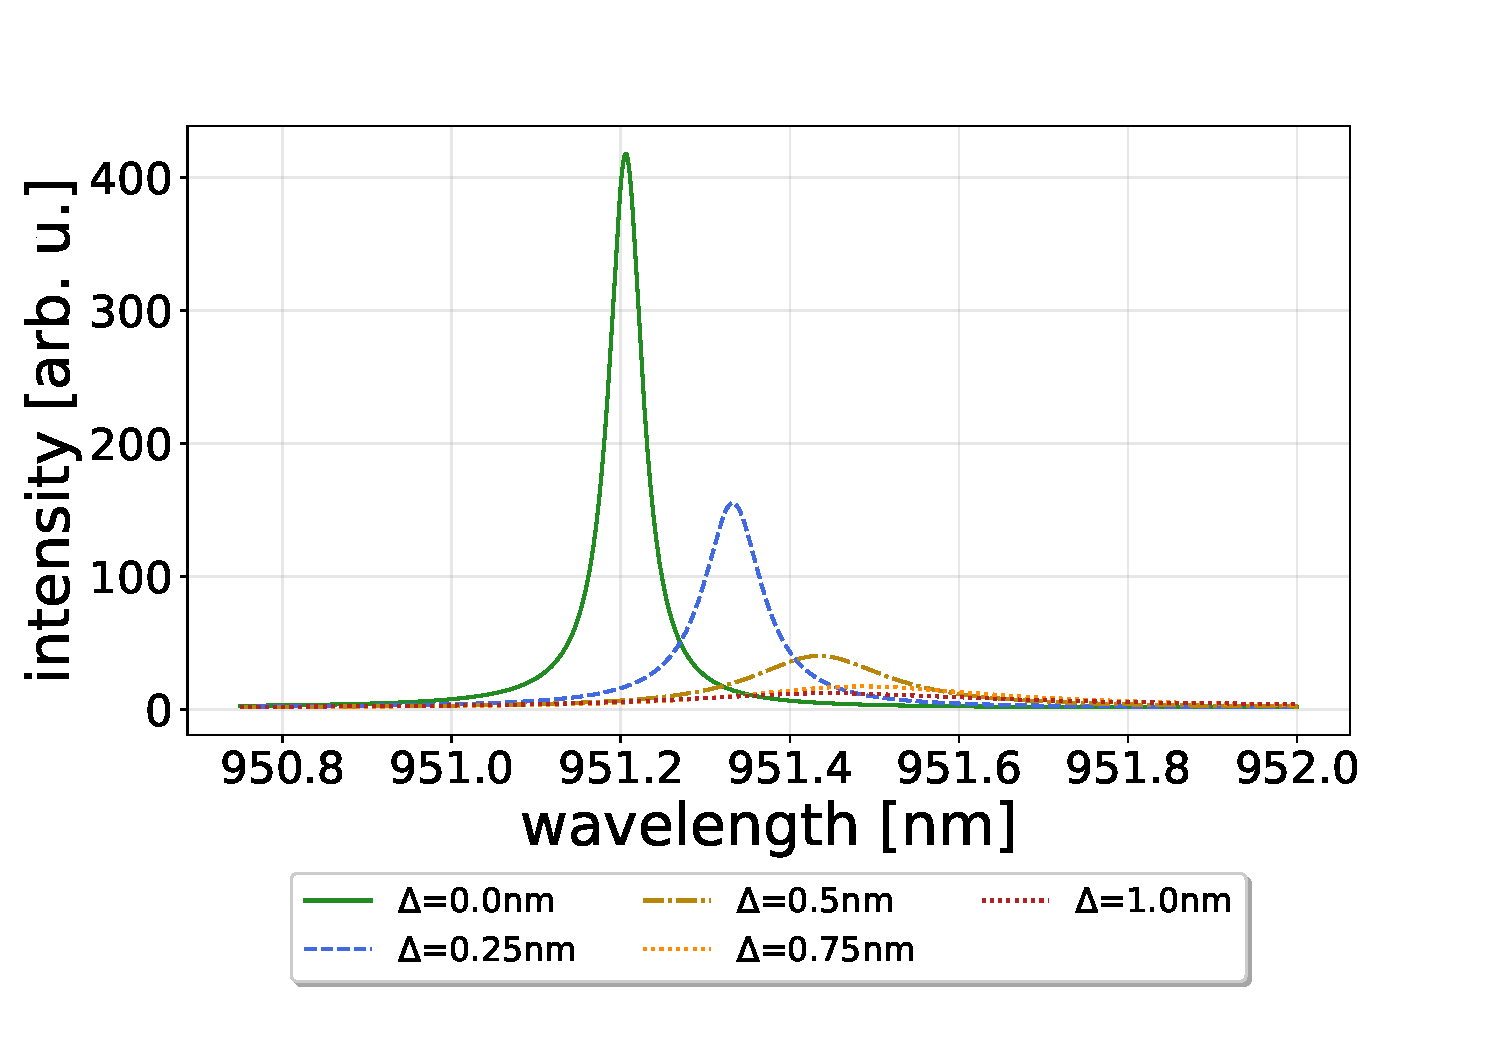
\includegraphics[width=\textwidth]{figures/detuning_scan_double_fano_30um_intracavity.pdf}
        \caption{}
        \label{fig:detuning_scan_intracavity}
    \end{subfigure}
    \caption{In (a) is seen lossless double Fano transmission spectra for increasing value of the detuning $\Delta = |\lambda_{0} - \lambda_{0}^{\prime}|$. It is readily seen that the transmission wavelength $\lambda_t = (\lambda_{0} + \lambda_{0}^{\prime})/2$ becomes higher, and that the linewidth likewise becomes larger with increasing detuning. (b) shows the intracavity spectra corresponding to the transmission spectra in (a) normalized by each their maximum value, shown in (c), in order to preserve readability.}
    \label{fig:detuning_scans}
\end{figure}

It is readily seen that with increasing positive detuning, relative to the resonant wavelength of the unchanged Fano mirror, the peak shifts to higher wavelengths, which in itself is easily seen from eq. (\ref{eq:transmission_wavelength}). The linewidth is also seen to increase with the detuning, and the peak will eventually collapse when the overlap between the guided-mode resonance profiles of the two Fano mirrors becomes too small to sustain the Fano resonance. This collapse was seen for examples of higher losses, and will be evident in later sections. Figure \ref{fig:detuning_scan_intracavity_normalized} shows the intracavity spectra corresponding to the transmission spectra in figure \ref{fig:detuning_scan} normalized by their respective maximum values plotted in figure \ref{fig:detuning_scan_intracavity_max_values} in order to preserve readability. The intracavity spectra provides valuable insight into the mode density inside the cavity for the different values of $\Delta$, and considering the significant difference of $\propto 10^4$ in the maximum value for the intensity, a mode density decrease is, though qualitative, clearly shown by figure \ref{fig:detuning_scan_intracavity_max_values}.  

It is clearly demonstrated by figures \ref{fig:detuning_scan}, \ref{fig:detuning_scan_intracavity_normalized} and \ref{fig:detuning_scan_intracavity_max_values} that the spectral overlap is a very crucial parameter of the double Fano cavity, and is paramount in describing the cavity's ability to produce narrow Fano resonant structures. 

\subsubsection{Spacial detuning (lossless)} \label{sec:spacial_detuning}

As mentioned above in section \ref{sec:spectral_detuning}, any spectral detuning gives rise to the potential of a spacial detuning as $2l = m\lambda$ must be fulfilled for any sustained plane-wave mode inside a normal incident optical cavity. We denote the length corresponding to the resonance wavelength of the unchanged Fano mirror as simply $l$, while the one for the detuned Fano mirror will be denoted as $l^{\prime}$. Previously we assumed that the optimal length of a detuned double Fano cavity is the one where the so-called transmission wavelength is given as 
\begin{equation}
    \lambda_t = \frac{\lambda_{0} + \lambda_{0}^{\prime}}{2}.
\end{equation}
And while this does turn out to be a good emprically justified assumption in the experimental part of this project, we will model and investigate the resonant length-dependence of the linewidth of the Fano resonance profile. 

\begin{figure}[h!]
    \centering
    \begin{subfigure}[b]{0.49\textwidth}
        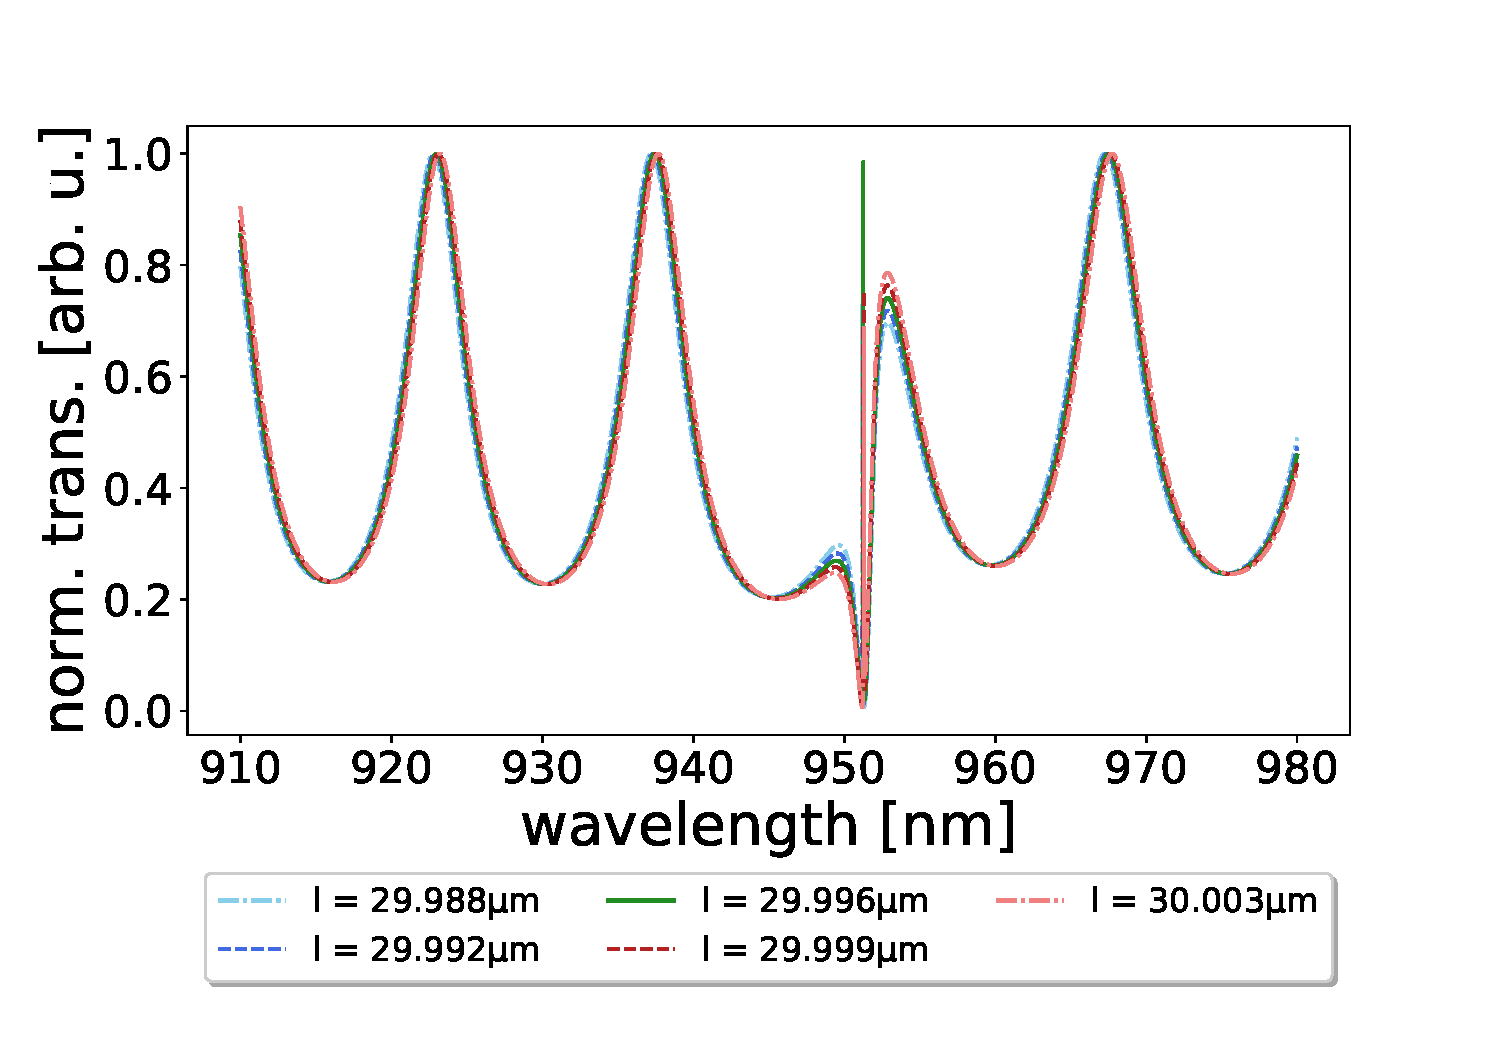
\includegraphics[width=\textwidth]{figures/small_detuning_length_scan_long.pdf}
        \caption{}
        \label{fig:detuned_small_length_scan_long}
    \end{subfigure}
    \begin{subfigure}[b]{0.49\textwidth}
        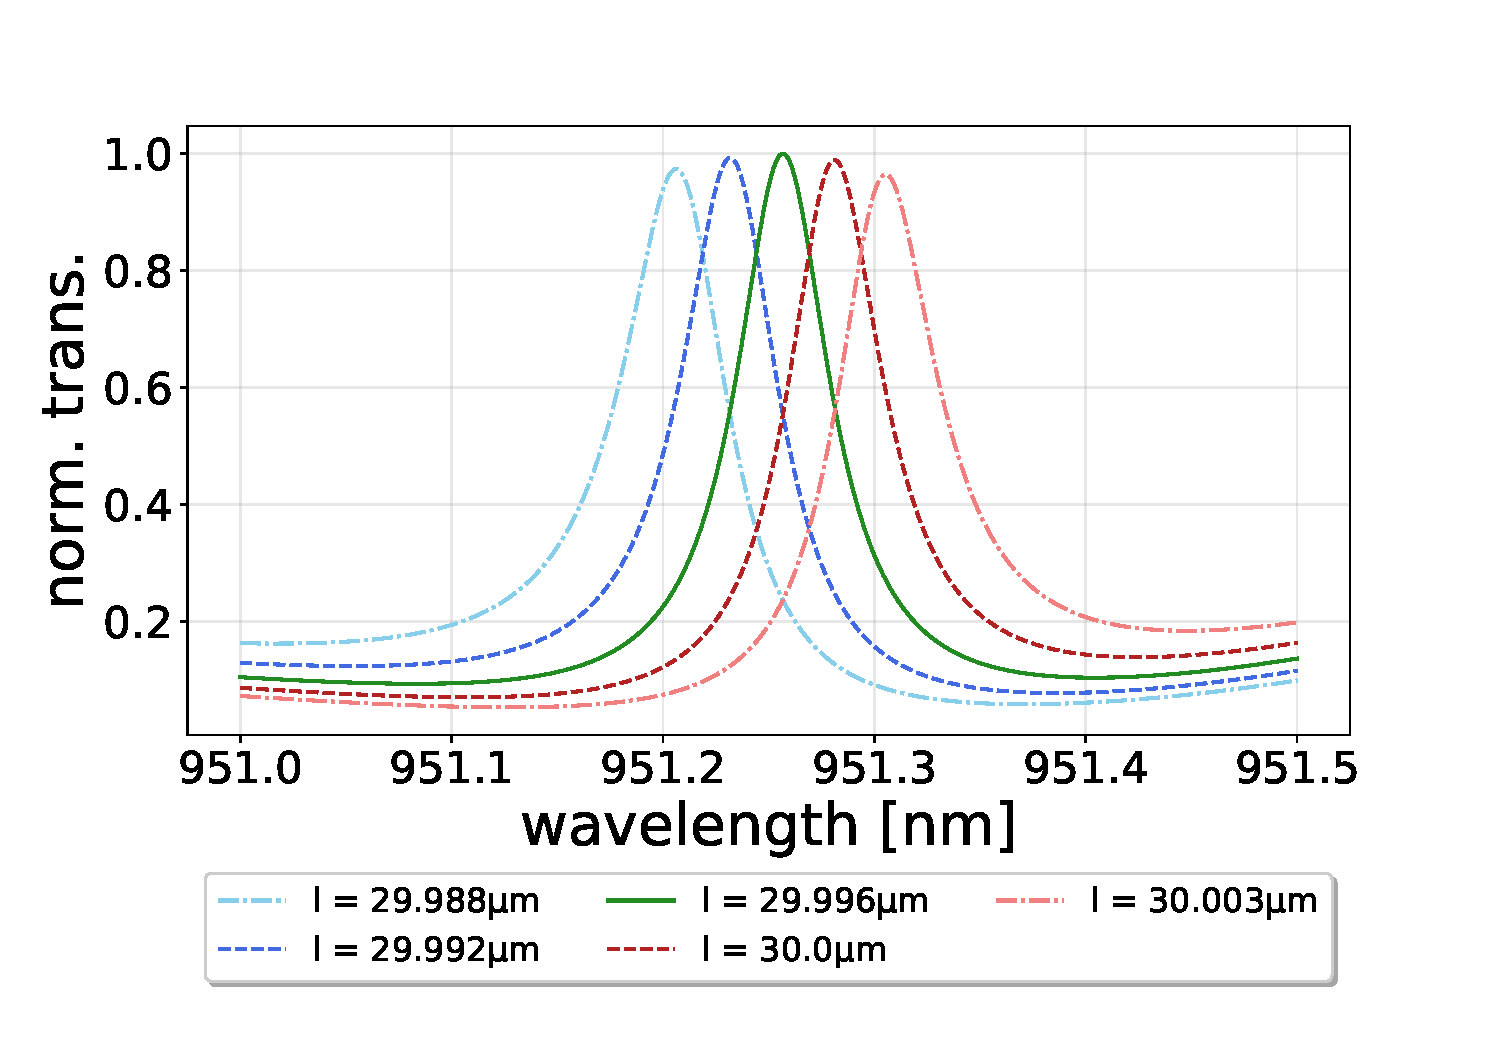
\includegraphics[width=\textwidth]{figures/small_detuning_length_scan_short.pdf}
        \caption{}
        \label{fig:detuned_small_length_scan_short}
    \end{subfigure}
    \caption{(a) shows lossless long-range transmission spectra of double Fano cavities of lengths $l \rightarrow l^{\prime} \approx 30 \mu m$ with $\Delta = 0.1nm$. (b) shows the same spectra as seen in (a), zoomed in on the range around the transmission wavelength $\lambda_t$.}
    \label{fig:small_detuning_length_scans}
\end{figure}

Figure \ref{fig:small_detuning_length_scans} shows double Fano resonance transmission profiles plottet for varying cavity length $l \rightarrow l^{\prime}$ with detuning $\Delta = 0.1nm$. The long range wavelength scan in figure \ref{fig:detuned_small_length_scan_long} shows a well-defined off-resonance behavior, as the detuning is barely visible on this scale, while the peak height on resonance is already visibly affected. The immediate off-resonance spectra also shows visible changes as the peak "background" level depend heavily on the location of the overall resonance.  

Figure \ref{fig:detuned_small_length_scan_short} shows the same spectra, but enhanced around the resonance wavelength. This shows that the substantiel guided-mode overlap, and thus small detuning, is enough to detect significant changes in the reosnance spectra. The shifting of the peak position is evident, but the most prominent change is seen in the peak height, which is reduced from $1$ when $\lambda_t = (lambda_0 + \lambda_0^{\prime})/2$ to around $0.8$ when $\lambda_t = lambda_0$ or $\lambda_t = \lambda_0^{\prime}$.

\begin{figure}[h!]
    \centering
    \begin{subfigure}[b]{0.49\textwidth}
        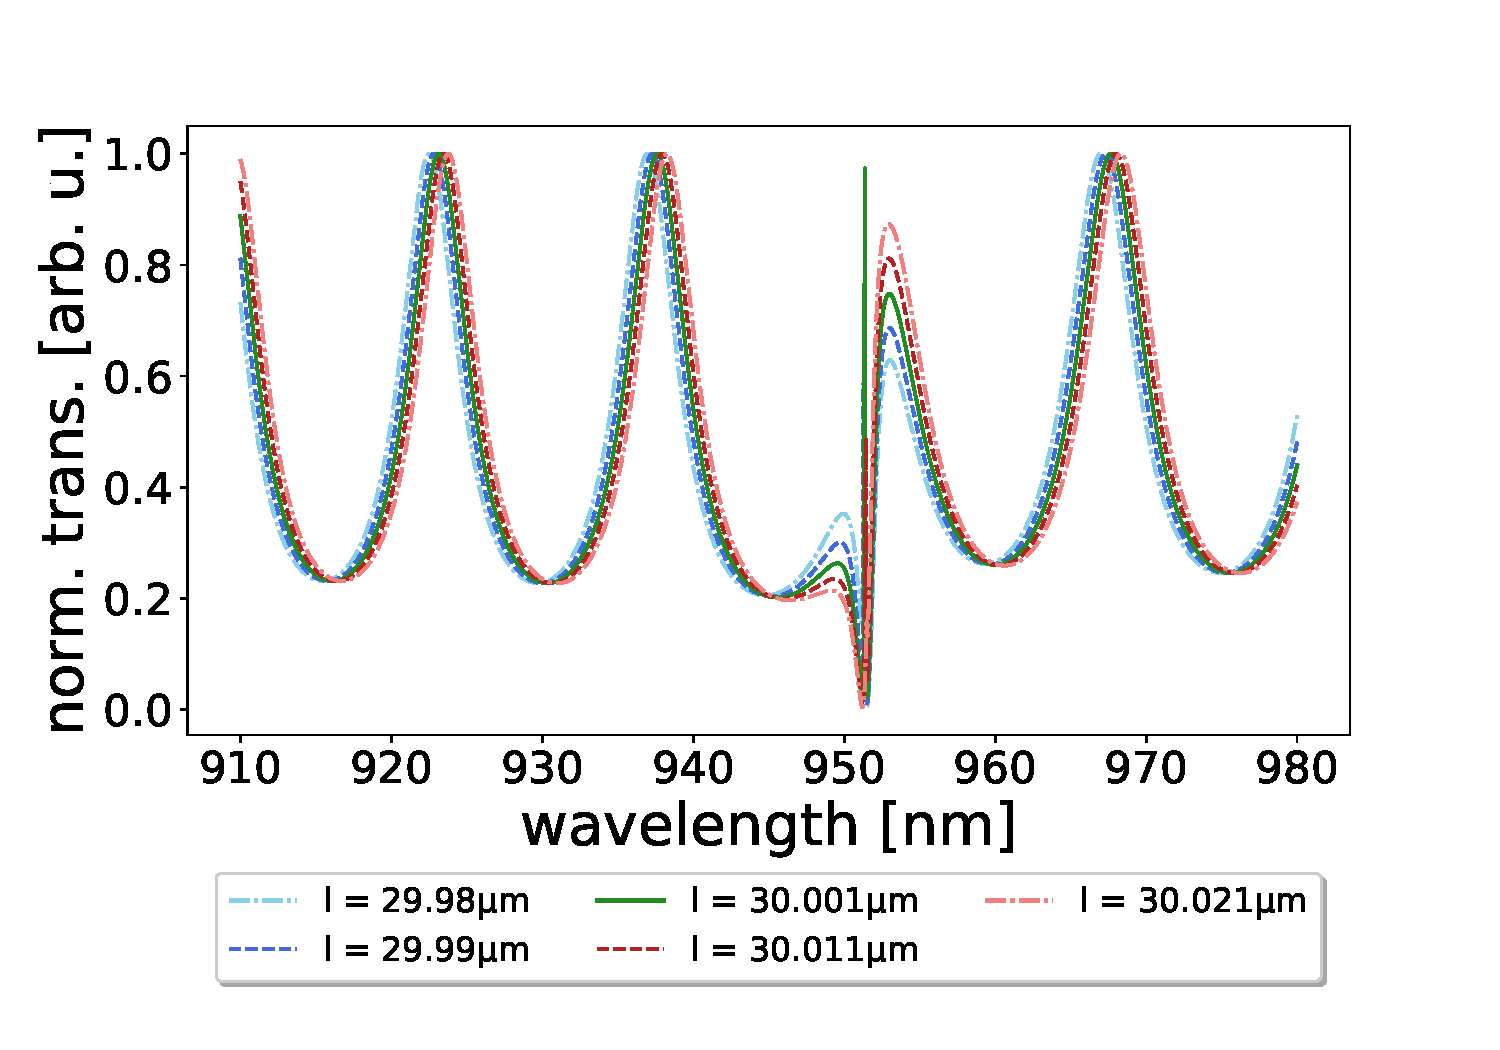
\includegraphics[width=\textwidth]{figures/medium_detuning_length_scan_long.pdf}
        \caption{}
        \label{fig:detuned_length_scan_long}
    \end{subfigure}
    \begin{subfigure}[b]{0.49\textwidth}
        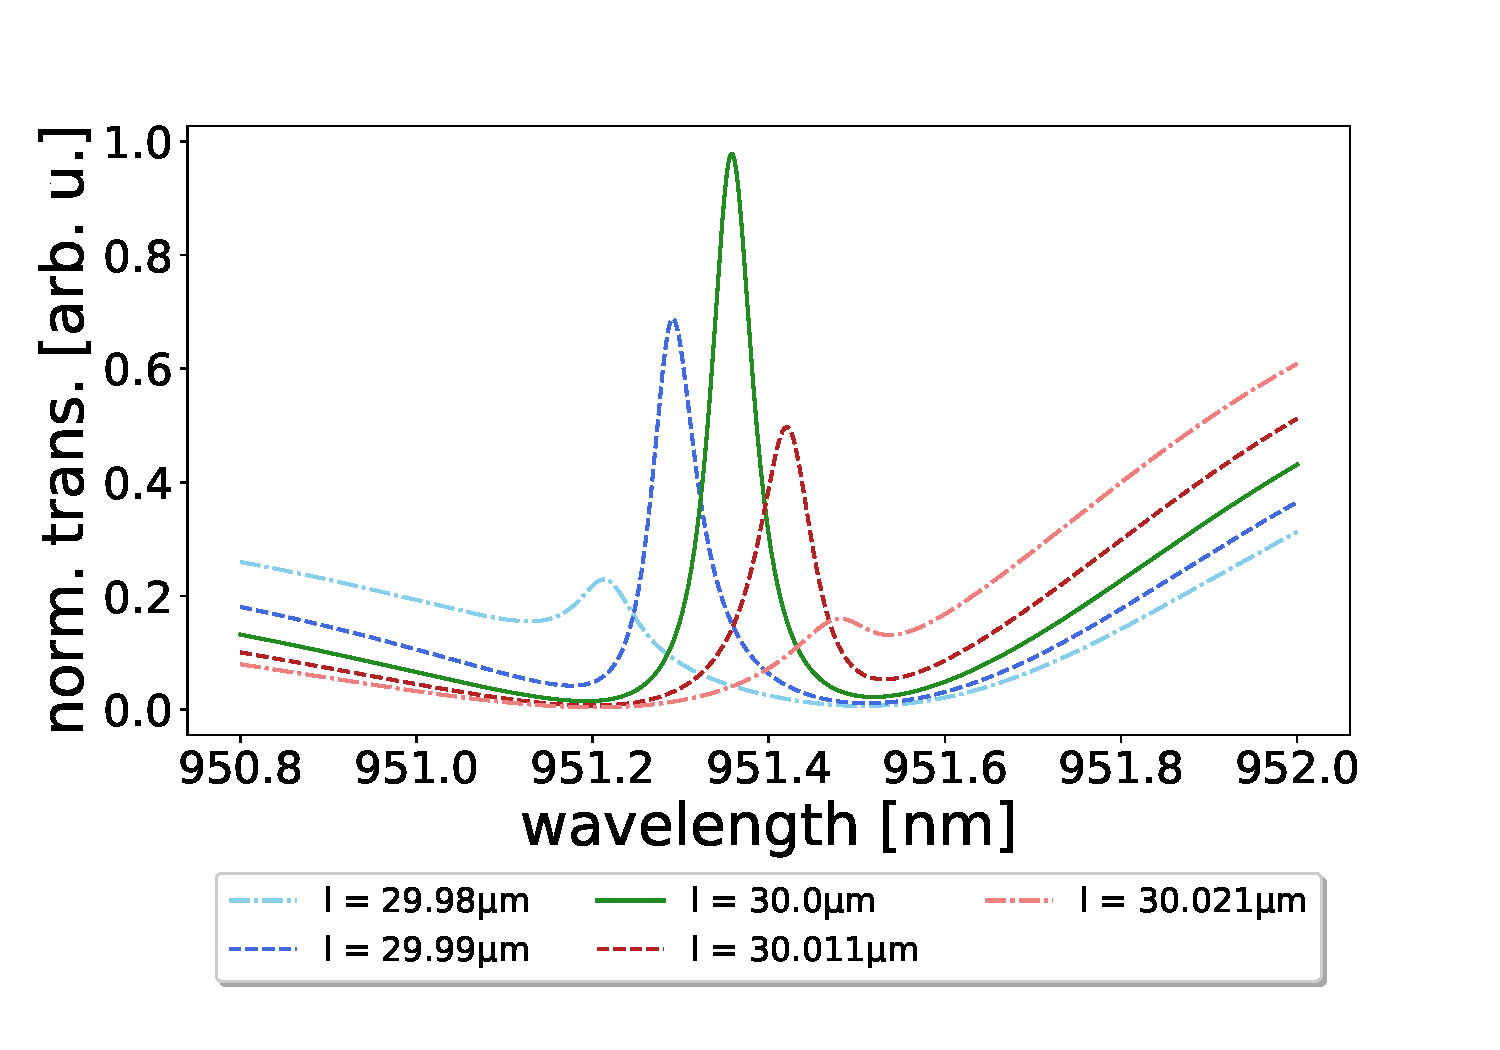
\includegraphics[width=\textwidth]{figures/medium_detuning_length_scan_short.pdf}
        \caption{}
        \label{fig:detuned_length_scan_short}
    \end{subfigure}
    \caption{(a) shows lossless long-range transmission spectra of double Fano cavities of lengths $l \rightarrow l^{\prime} \approx 30 \mu m$ with $\Delta = 0.3nm$. (b) shows the same spectra as seen in (a), zoomed in on the range around the transmission wavelength $\lambda_t$.}
    \label{fig:mid_detuning_length_scans}
\end{figure}

Figure \ref{fig:mid_detuning_length_scans} shows similar transmission profiles as in figure \ref{fig:small_detuning_length_scans}, only with an increased detuning of $\Delta = 0.3$nm. Looking at the long range scan in figure {\ref{fig:detuned_length_scan_long}} and comparing with the one in figure \ref{fig:detuned_small_length_scan_long}, it is seen that the displacement of the off-resonance Fabry-Perot like fringes have increased with the slightly higher detuning. This is not surprising as the Fabry-Perot cavity modes, like any other interference pattern inside a cavity must fulfill the brightness identity $2l = m \lambda$. Furthermore, the immediate off-resonance regime shows an increase in the intensity displacement when compared with the less detuned example. 

Figure \ref{fig:detuned_length_scan_short}, which shows the spectra enhanced around the resonance position, provides a more detailed image of what happens to the transmission profiles as a function of the cavity length. Here it is seen that the peaks at the edges of the length interval have varied even more in shape, height and linewidth than in figure \ref{fig:detuned_length_scan_short}. In short, the increased detuning has also increased the fractional length-dependence of the double Fano cavity transmission profile. Here it must however be noted here that the range in which the cavity length is scanned is increased with the detuning. So the length-dependence is fractional in the sense that the step size is here defined by the size of the interval.

\begin{figure}[h!]
    \centering
    \begin{subfigure}[b]{0.49\textwidth}
        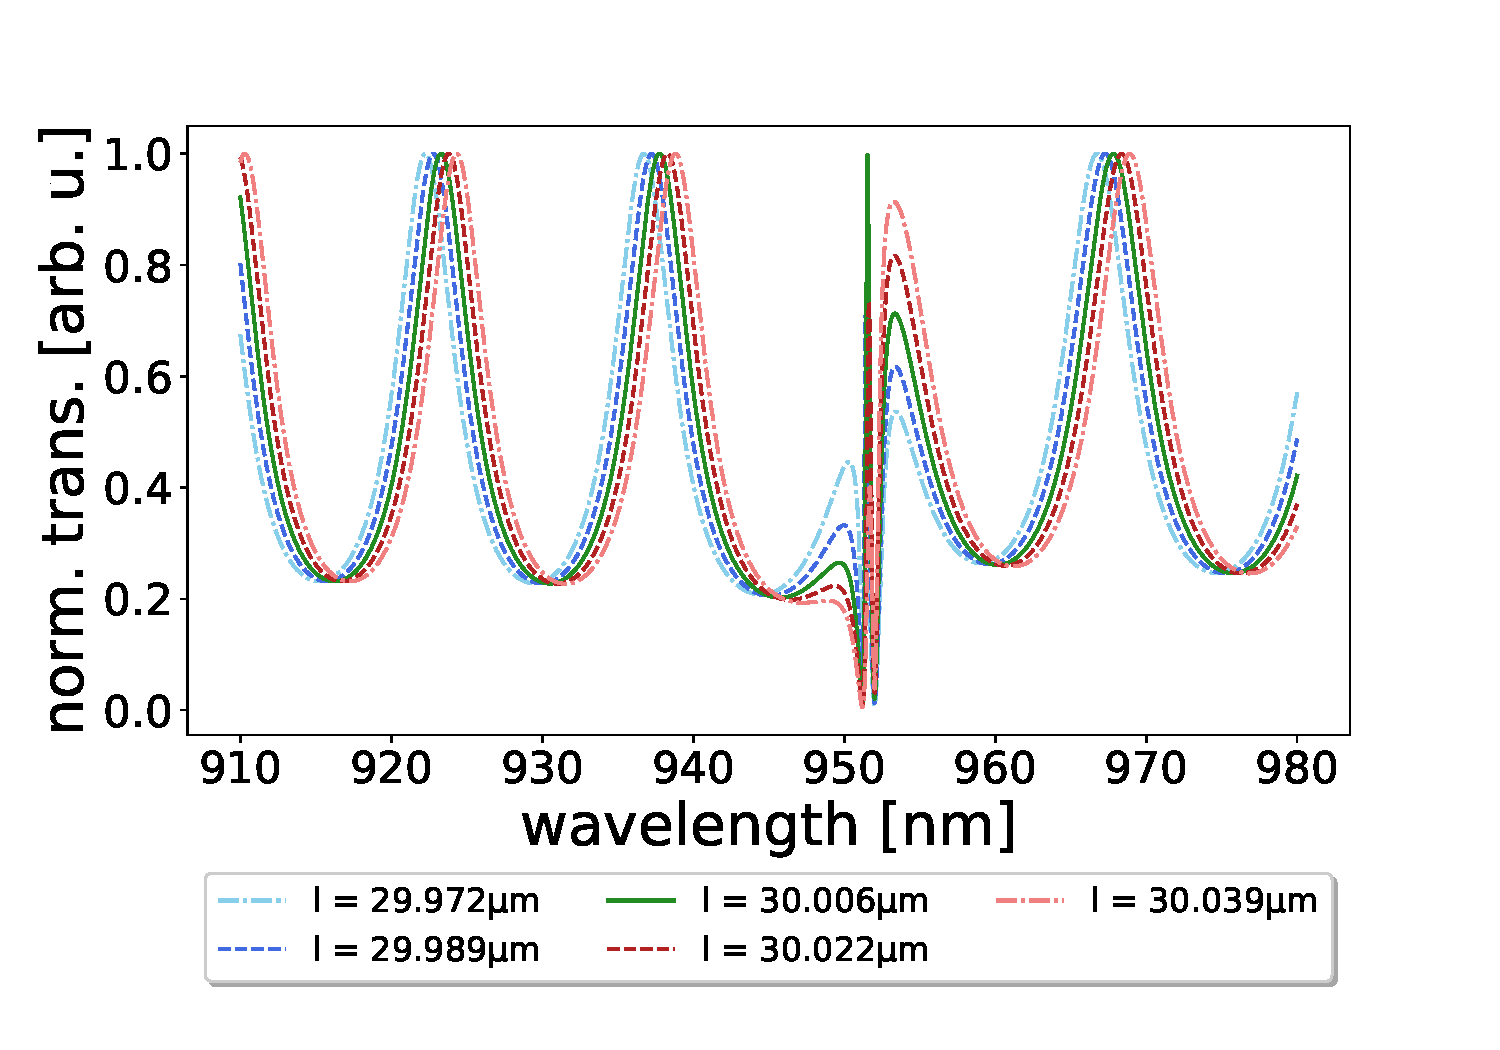
\includegraphics[width=\textwidth]{figures/large_detuning_length_scan_long.pdf}
        \caption{}
        \label{fig:detuned_large_length_scan_long}
    \end{subfigure}
    \begin{subfigure}[b]{0.49\textwidth}
        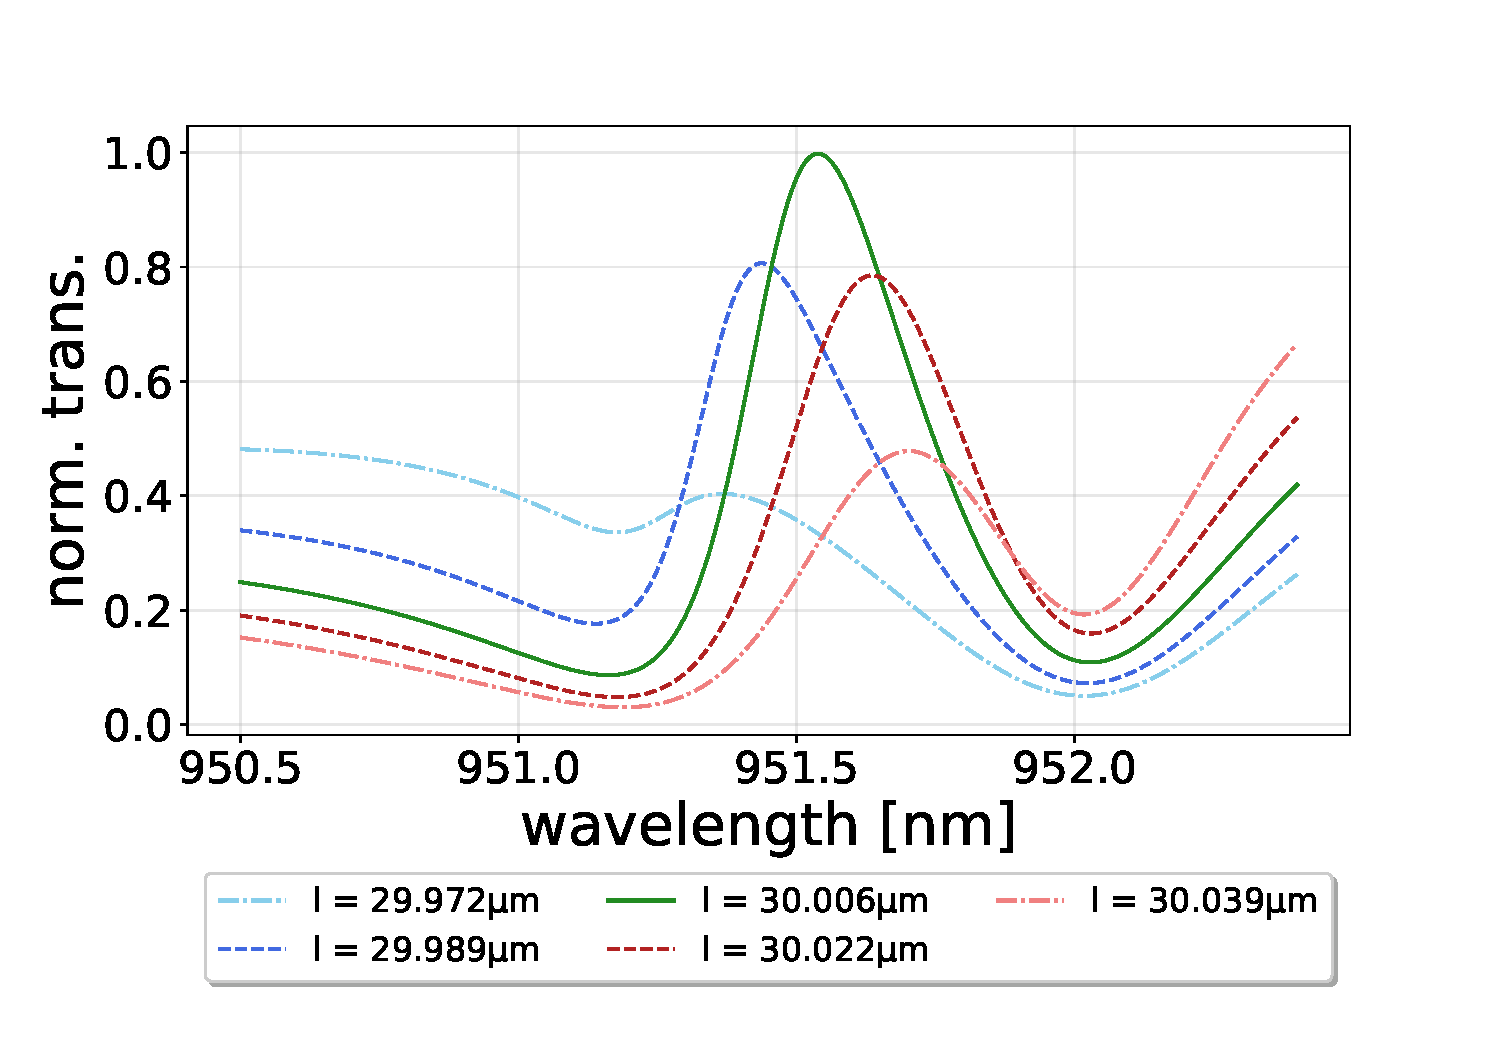
\includegraphics[width=\textwidth]{figures/large_detuning_length_scan_short.pdf}
        \caption{}
        \label{fig:detuned_large_length_scan_short}
    \end{subfigure}
    \caption{(a) shows lossless long-range transmission spectra of double Fano cavities of lengths $l \rightarrow l^{\prime} \approx 30 \mu m$ with $\Delta = 0.8nm$. (b) shows the same spectra as seen in (a), zoomed in on the range around the transmission wavelength $\lambda_t$.}
    \label{fig:large_detuning_length_scans}
\end{figure}

Figure \ref{fig:large_detuning_length_scans} shows the effect of a relatively large detuning of $\Delta = 0.8$nm. This is simply included for a visual representation of a detuning which is considered "too large" for any practical use. The long range scan in figure \ref{fig:detuned_large_length_scan_long} shows that the Fabry-Perot like fringes are now even more displaced, and figure \ref{fig:detuned_large_length_scan_short} showing the spectra enhanced around the resonance wavelength shows roughly the same trend as in figure \ref{fig:detuned_length_scan_short}, only that this example is greatly broadened in comparison. It is though noted, that while broadened, the Fano resonance mode is sustained even for the relatively large detuning.

In order to get a clear qualitative picture of the double Fano cavity transmission profile as a function of both cavity length and wavelength, we visualize the varying of both in a heat map and let the color indicate the transmission intensity. This is shown in figure \ref{fig:cmap_single} which depicts a lossless cavity of length $l\approx 30 \mu m$ and detuning $\Delta = 0.3$nm. Here the movement of the resonance peak as a function of the cavity length is clearly seen as a slope of the "line" representing the high intensity region due to the Fano resonance. 

\begin{figure}[h!]
    \centering
    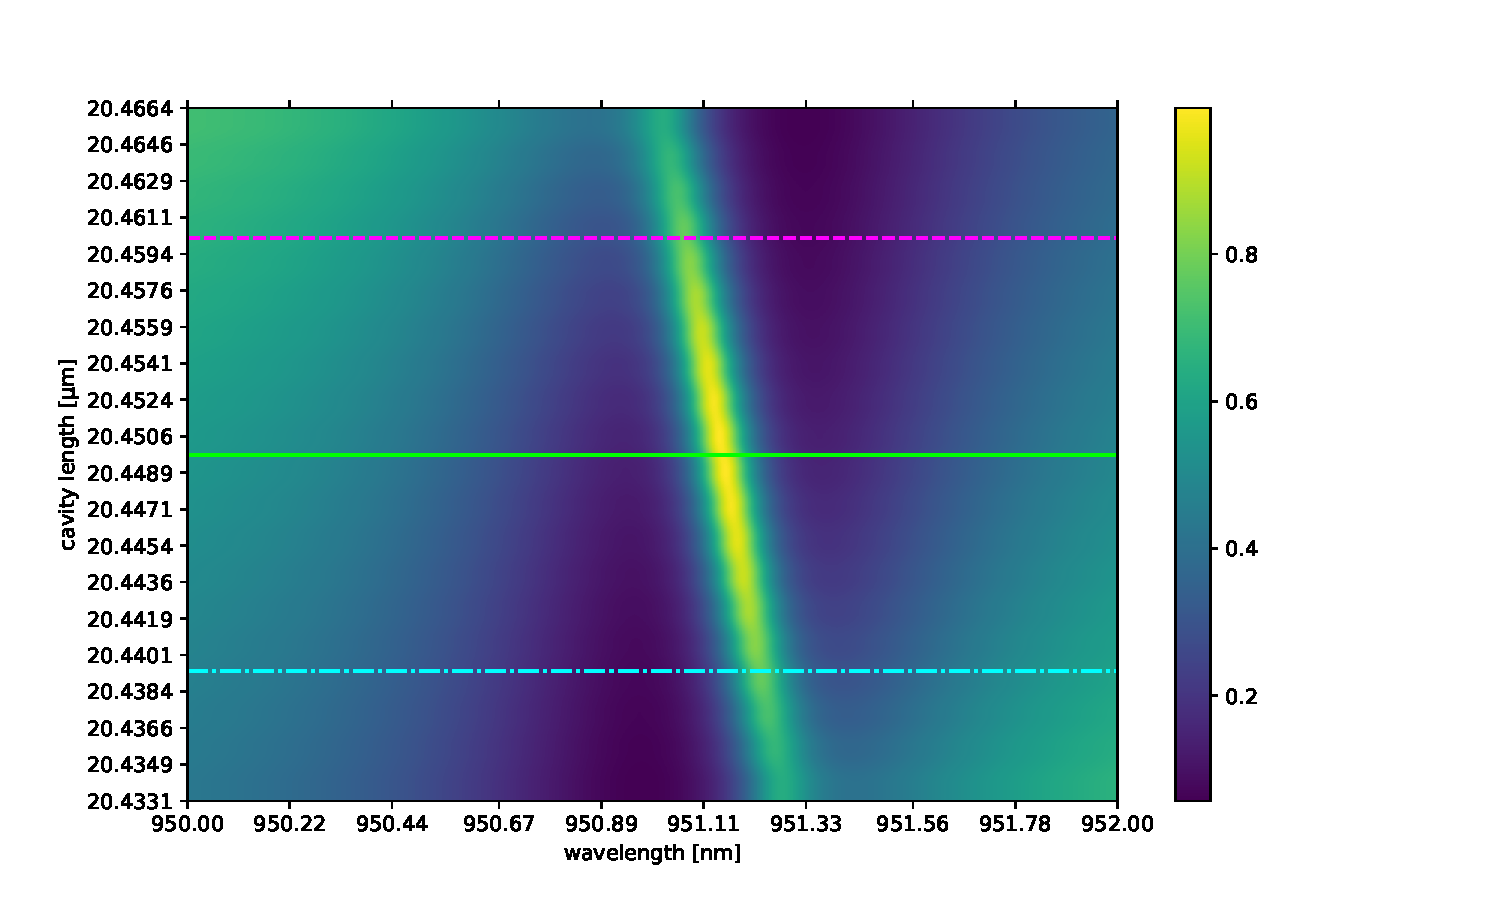
\includegraphics[width=0.7\textwidth]{figures/cmap_with_slice_indicators1.pdf}
    \caption{Heat map of the lossless double Fano cavity transmission as a function of wavelength and cavity lengths ranging $l \rightarrow l^{\prime} \approx 30 \mu m$ for $\Delta = 0.3$nm}
    \label{fig:cmap_single}
\end{figure}

\begin{figure}[h!]
    \centering
    \begin{subfigure}[b]{0.49\textwidth}
        \centering
        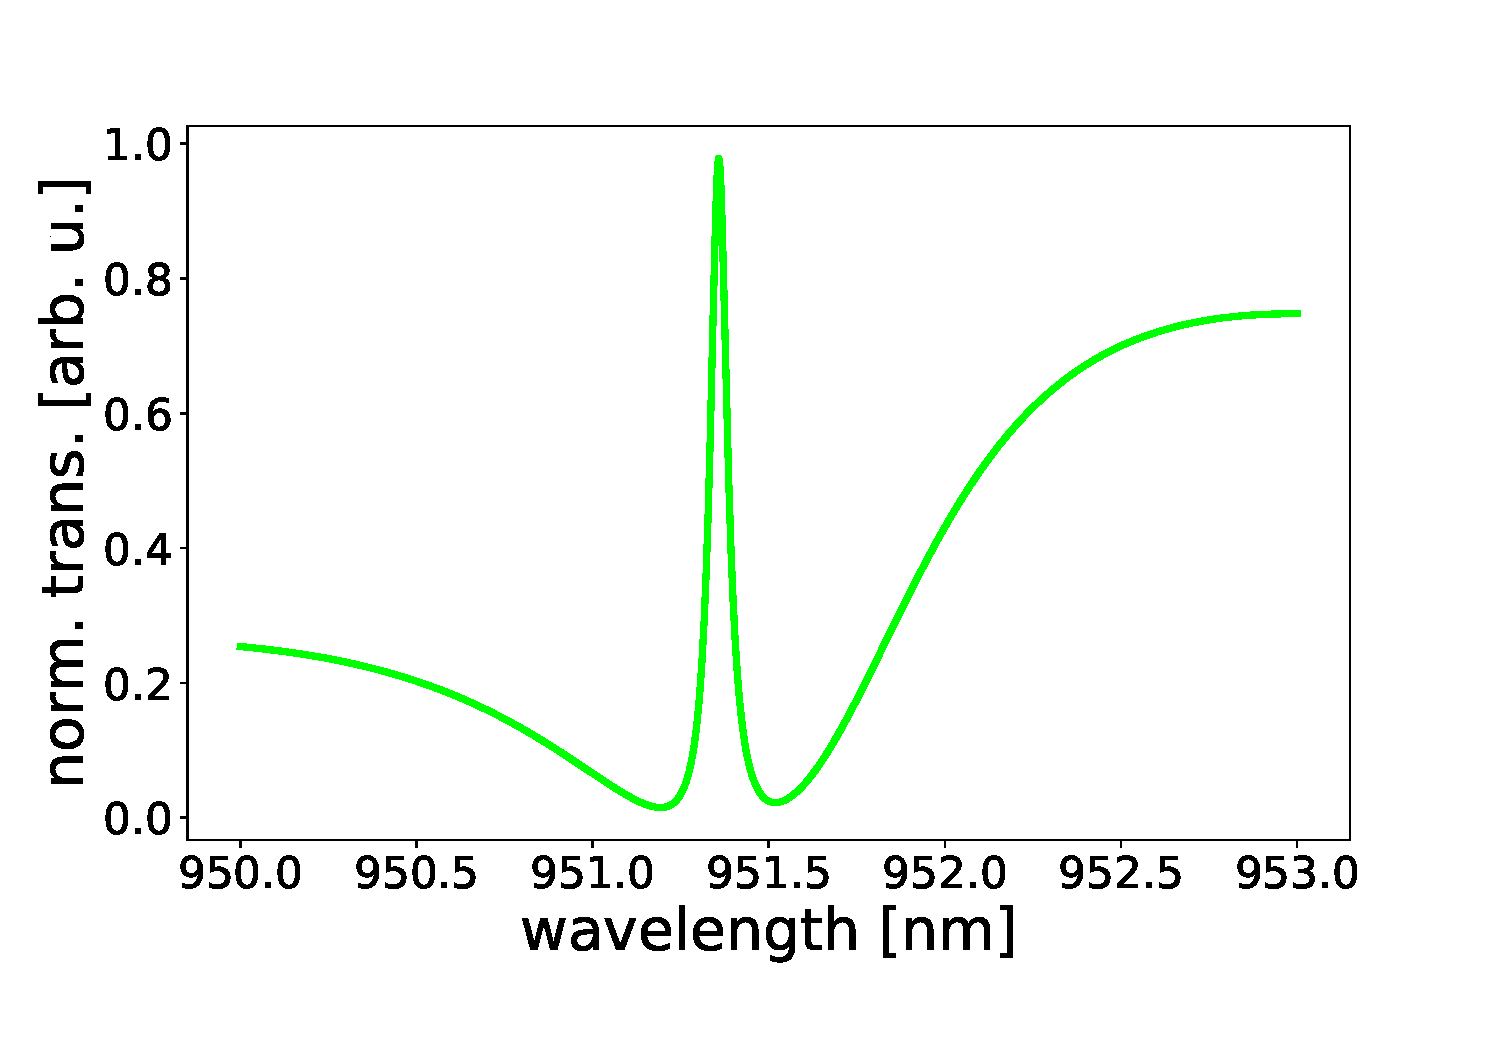
\includegraphics[width=\textwidth]{figures/cmap_slice1.pdf}
        \caption{}
        \label{fig:cmap_slice1}
    \end{subfigure}
    \begin{subfigure}[b]{0.49\textwidth}
        \centering
        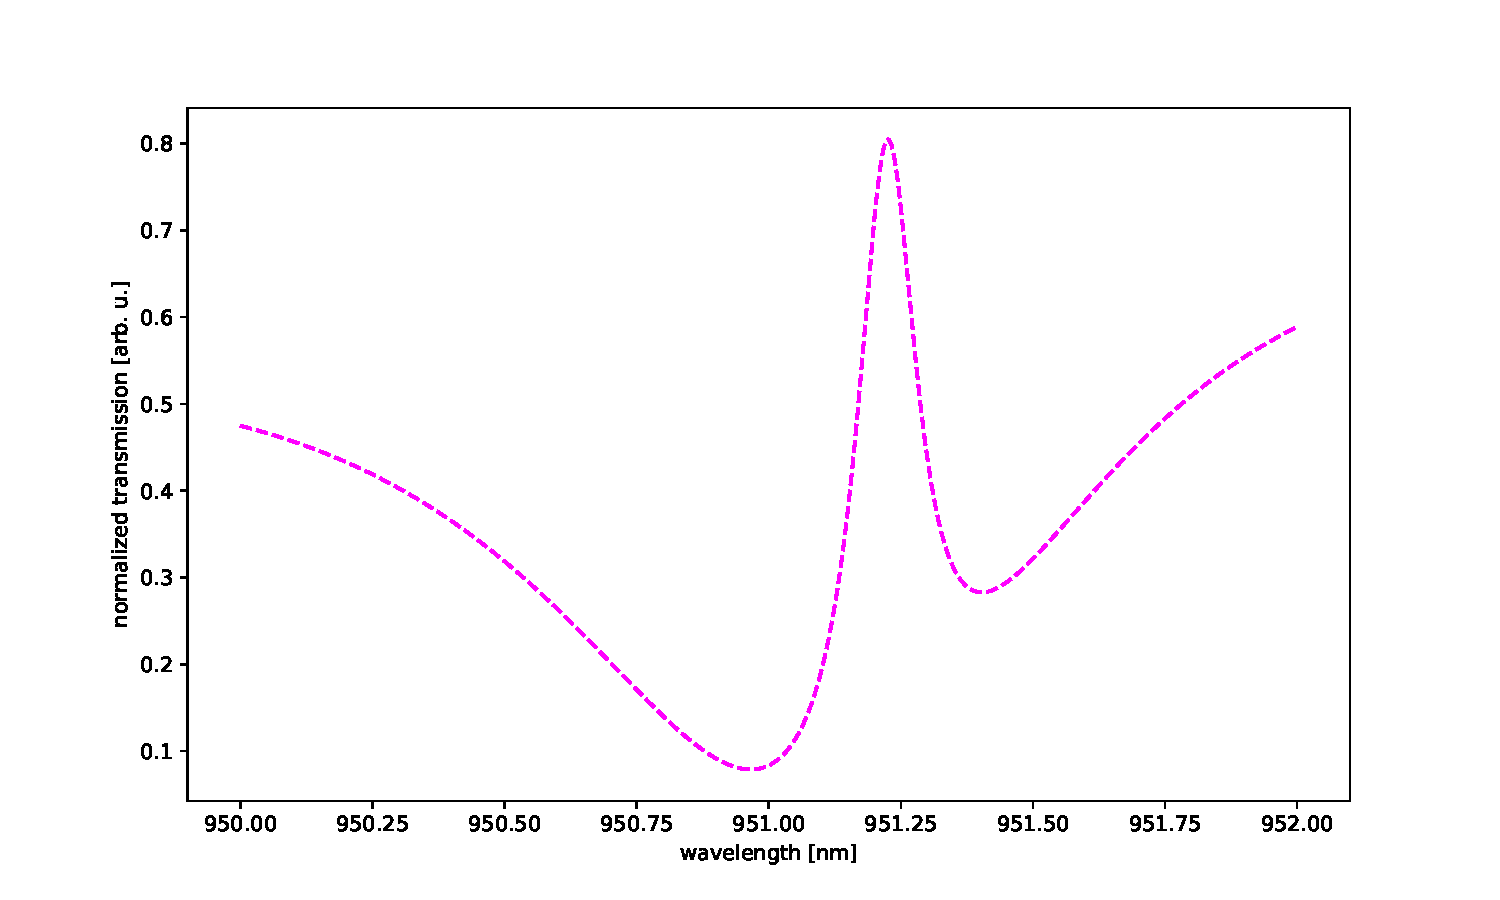
\includegraphics[width=\textwidth]{figures/cmap_slice2.pdf}
        \caption{}
        \label{fig:cmap_slice2}
    \end{subfigure}
    \begin{subfigure}[b]{0.49\textwidth}
        \centering
        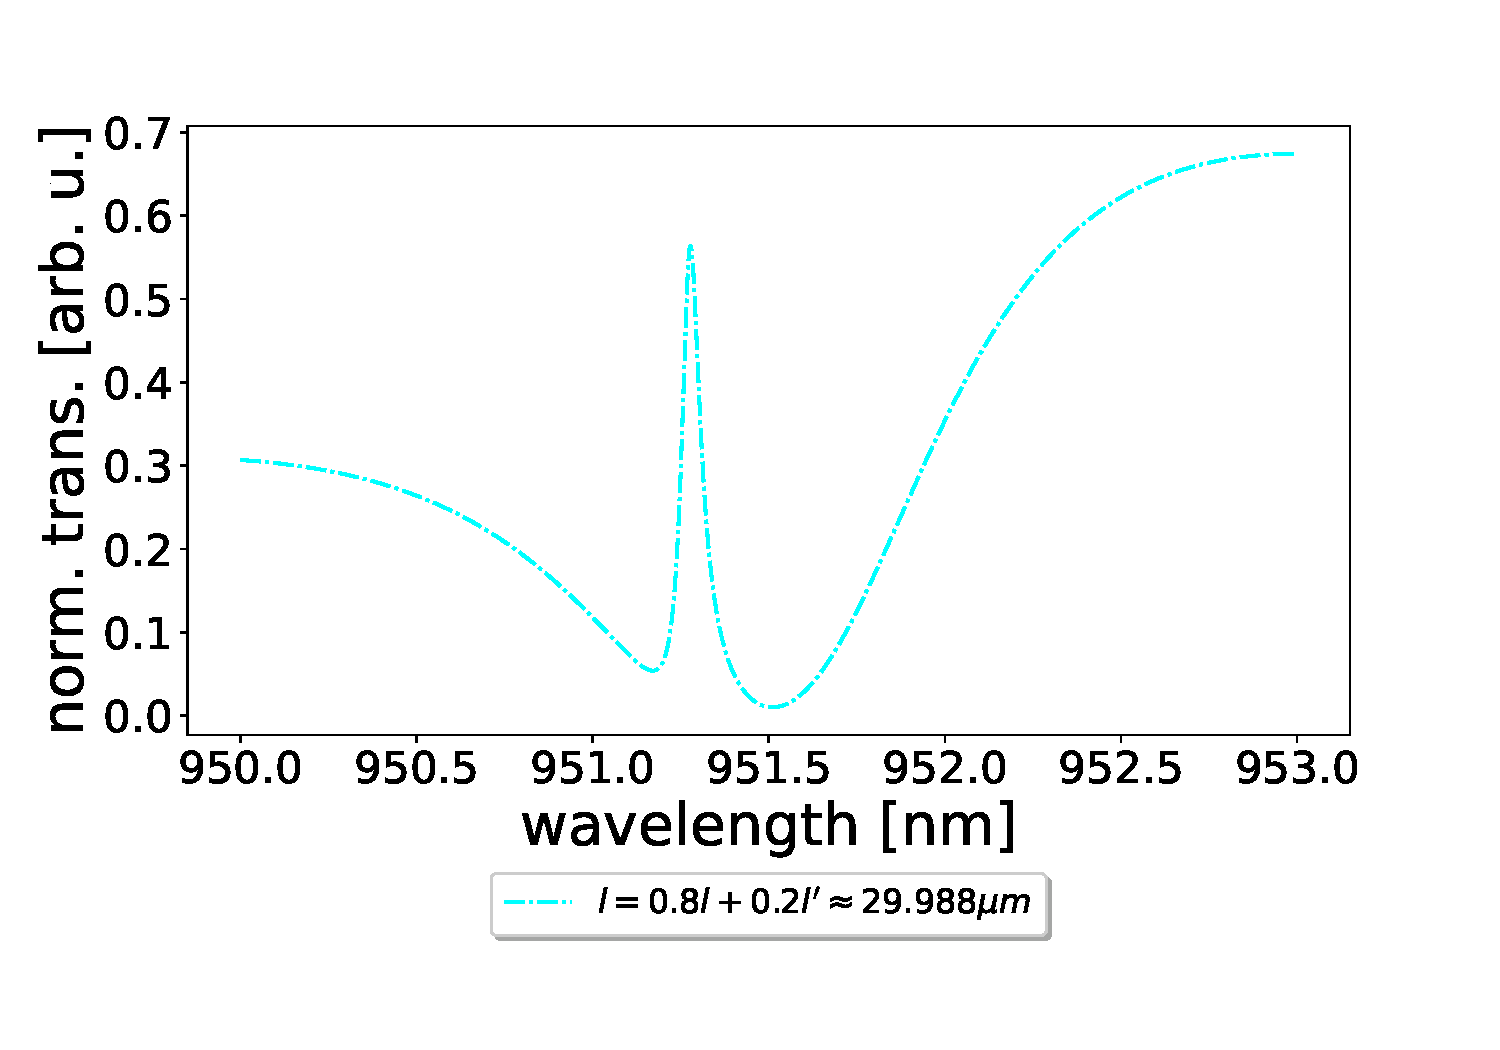
\includegraphics[width=\textwidth]{figures/cmap_slice3.pdf}
        \caption{}
        \label{fig:cmap_slice3}
    \end{subfigure}
    \begin{subfigure}[b]{0.49\textwidth}
        \centering
        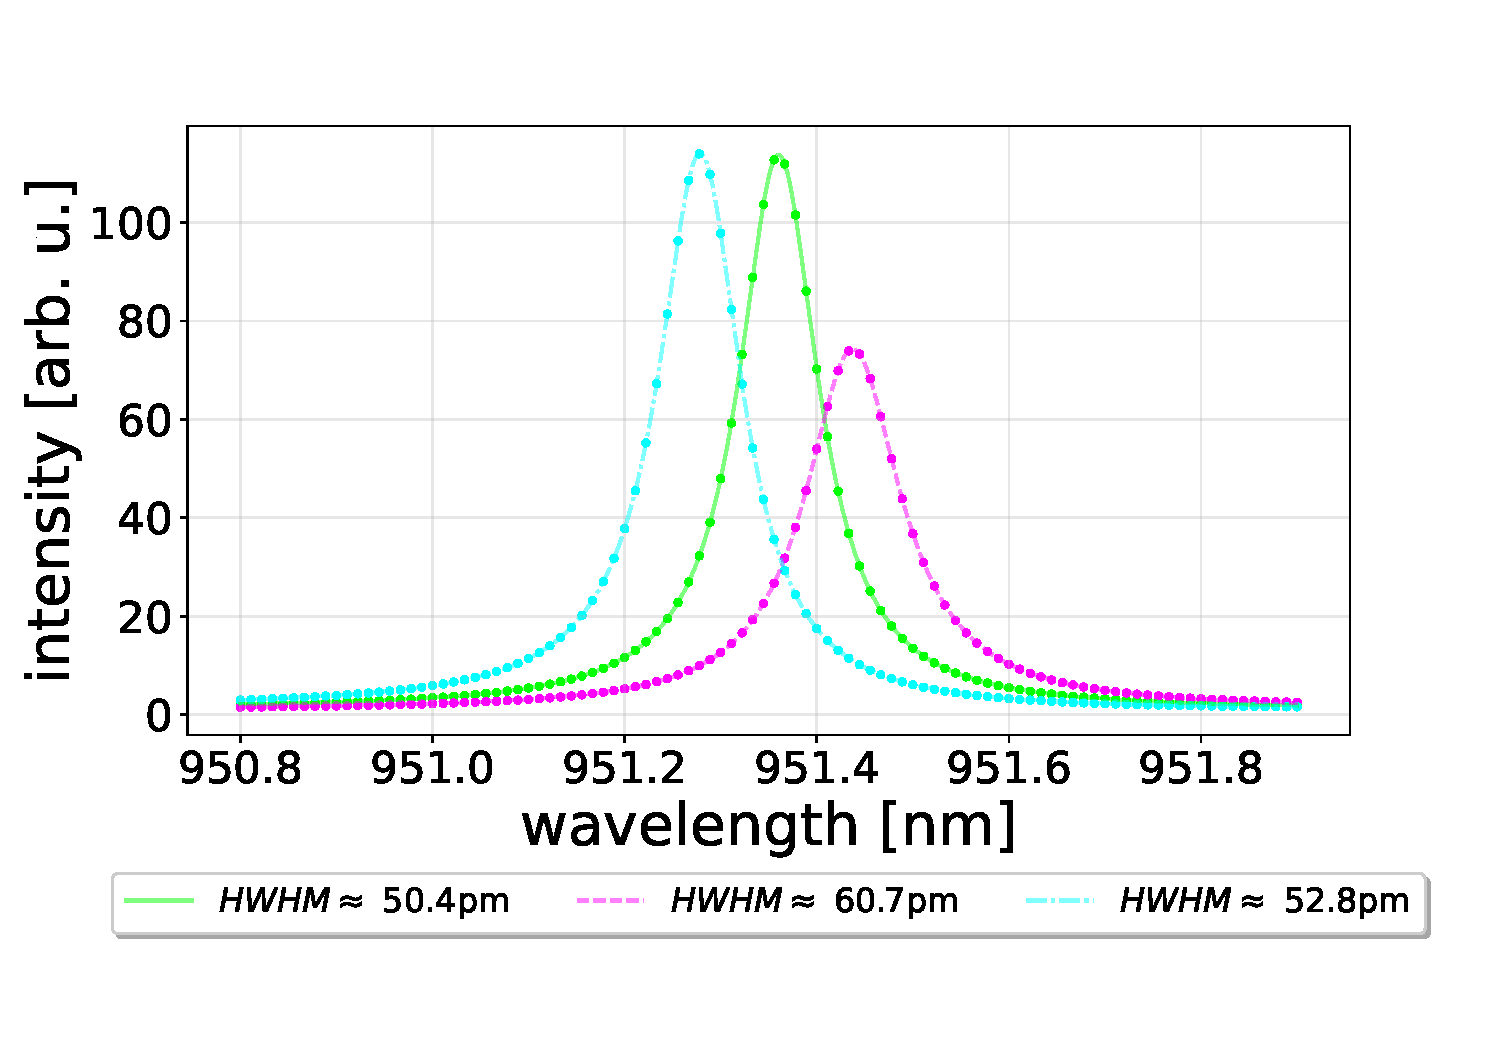
\includegraphics[width=\textwidth]{figures/cmap_lws.pdf}
        \caption{}
        \label{fig:cmap_lws}
    \end{subfigure}
    \caption{(a), (b) and (c) show slices of the heat map in figure \ref{fig:cmap_single} indicated by their respective color an line type in order to compare different cavity lenghts. (d) show intracavity spectra of the peaks in (a), (b) and (c) with corresponding least squares fits and linewidths found as parameters hereof. }
    \label{fig:cmap_slices}
\end{figure}

Considering only the heat map, it is not easily visible which cavity length is the optimal one, however, the \emph{magenta}, \emph{cyan}, and \emph{limegreen} lines across the heat map indicate slices which are depicted separately in figure \ref{fig:cmap_slices}. It is seen by analysing the transmission profiles of the three cavities of specific lengths, how they vary in both position and linewidth. The lengths and corresponding linewidths are given as
\begin{equation}
    \begin{split}
        l_{magenta} = 0.2 l + 0.8 l^{\prime} &\rightarrow HWHM_{magenta} = 40.5pm\\ l_{cyan} = 0.8 l + 0.2 l^{\prime} &\rightarrow HWHM_{cyan} = 31.9pm\\ l_{lime} = (l + l^{\prime})/2 &\rightarrow HWHM_{lime} = 29.7pm.
    \end{split}
\end{equation}
It turns out that of the three cases, the \emph{lime} transmission profile seems optimal as it is the narrowest of the three, and seems to be more preferably positioned, i.e. it is more centered in and thus separated from the Fabry-Perot-like background. 

\begin{figure}[h!]
    \centering
    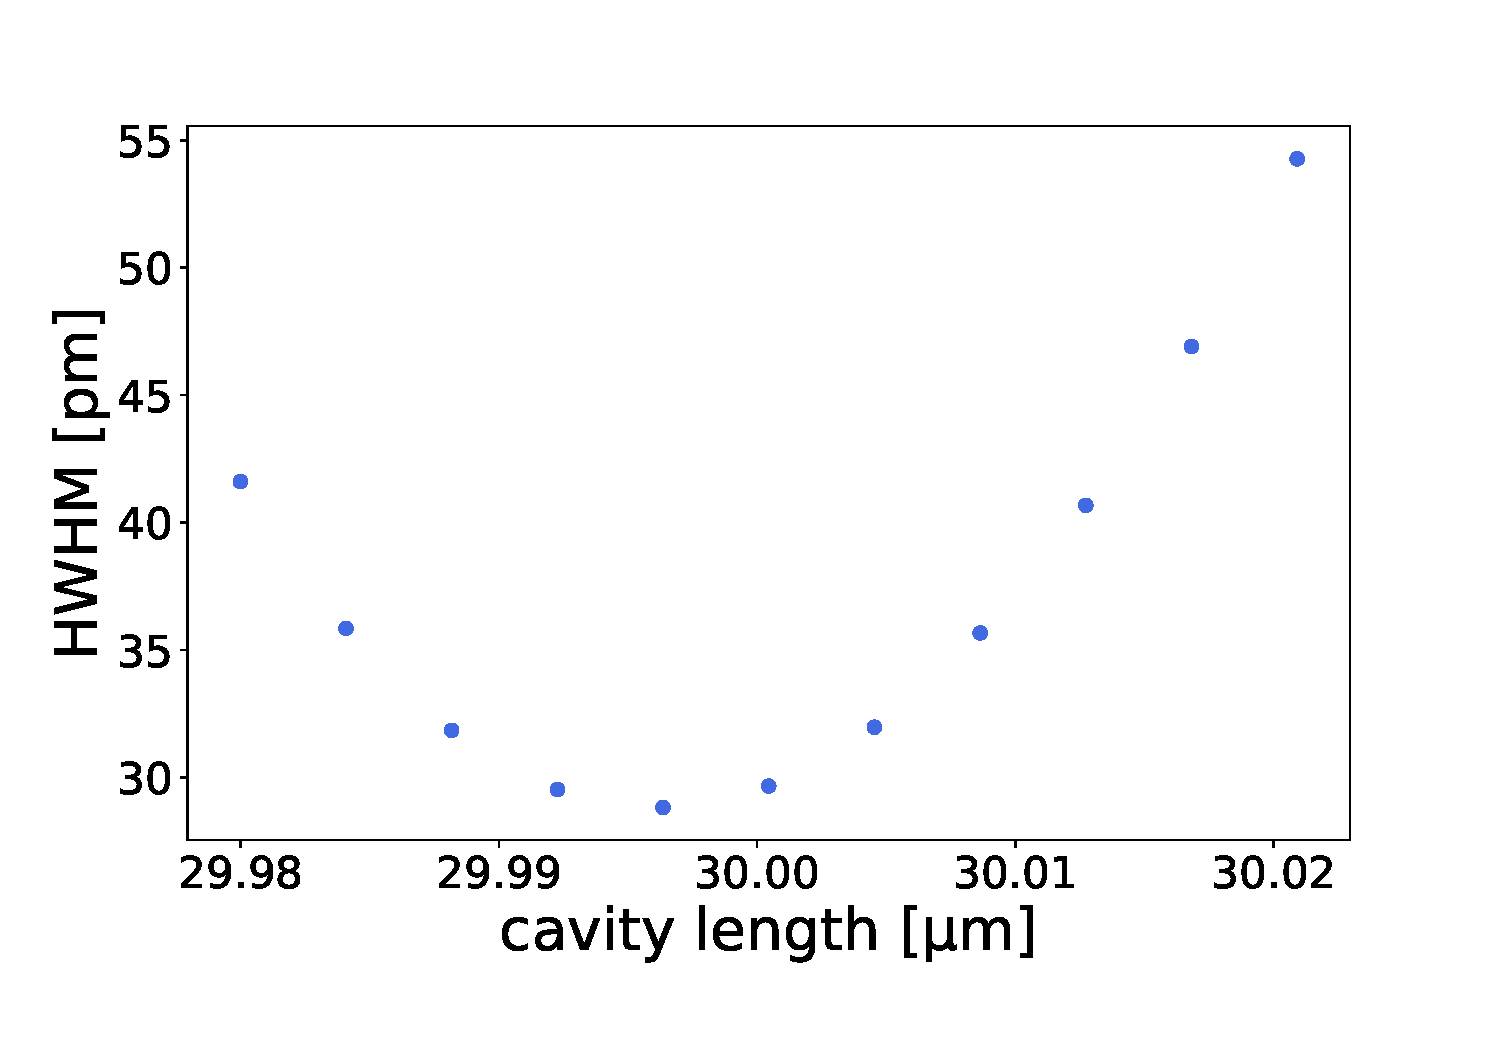
\includegraphics[width=0.7\textwidth]{figures/lw_vs_length_intracavity.pdf}
    \caption{Linewidth as a function of cavity length $l \rightarrow l^{\prime}$. Each point is found as a fitting parameter from a least squares fit to the generalized Fano model in eq. (\ref{eq:general_fano_model}) of lossless intracavity double Fano spectra.}
    \label{fig:lw_vs_l_scan}
\end{figure}

This trend is further examined in figure \ref{fig:lw_vs_l_scan} where the linewidths of intracavity spectra are shown as a function of the cavity length. The parameters used are the same as in figure \ref{fig:cmap_single} and the figure indicates that the optimal cavity length is definitely "somewhere in between" the two guided-,mode resonance lengths. However, it is also evident that the previous assumption for $\lambda_t$ is too simple to be general in this case. 

As a visual and qualitative representation of the effect of increasing the detuning $\Delta$, figure \ref{fig:cmaps_detuning} shows heat maps similar to the one in figure \ref{fig:cmap_single}, but for a range of values for the detuning $\Delta=0.01$nm$ \rightarrow \Delta=1.21$nm. It is readily seen that the aforementioned slope of the high intensity region, indicating the resonance peak, increases with the detuning. This is a representation of the peak moving to higher wavelengths, both for the optimal transmission wavelength and for the one closer to the detuned Fano mirror guided-mode resonance. The broadening of the peak is also displayed in a way that is, while only qualitative, convincing. 

\begin{figure}[h!]
    \centering
    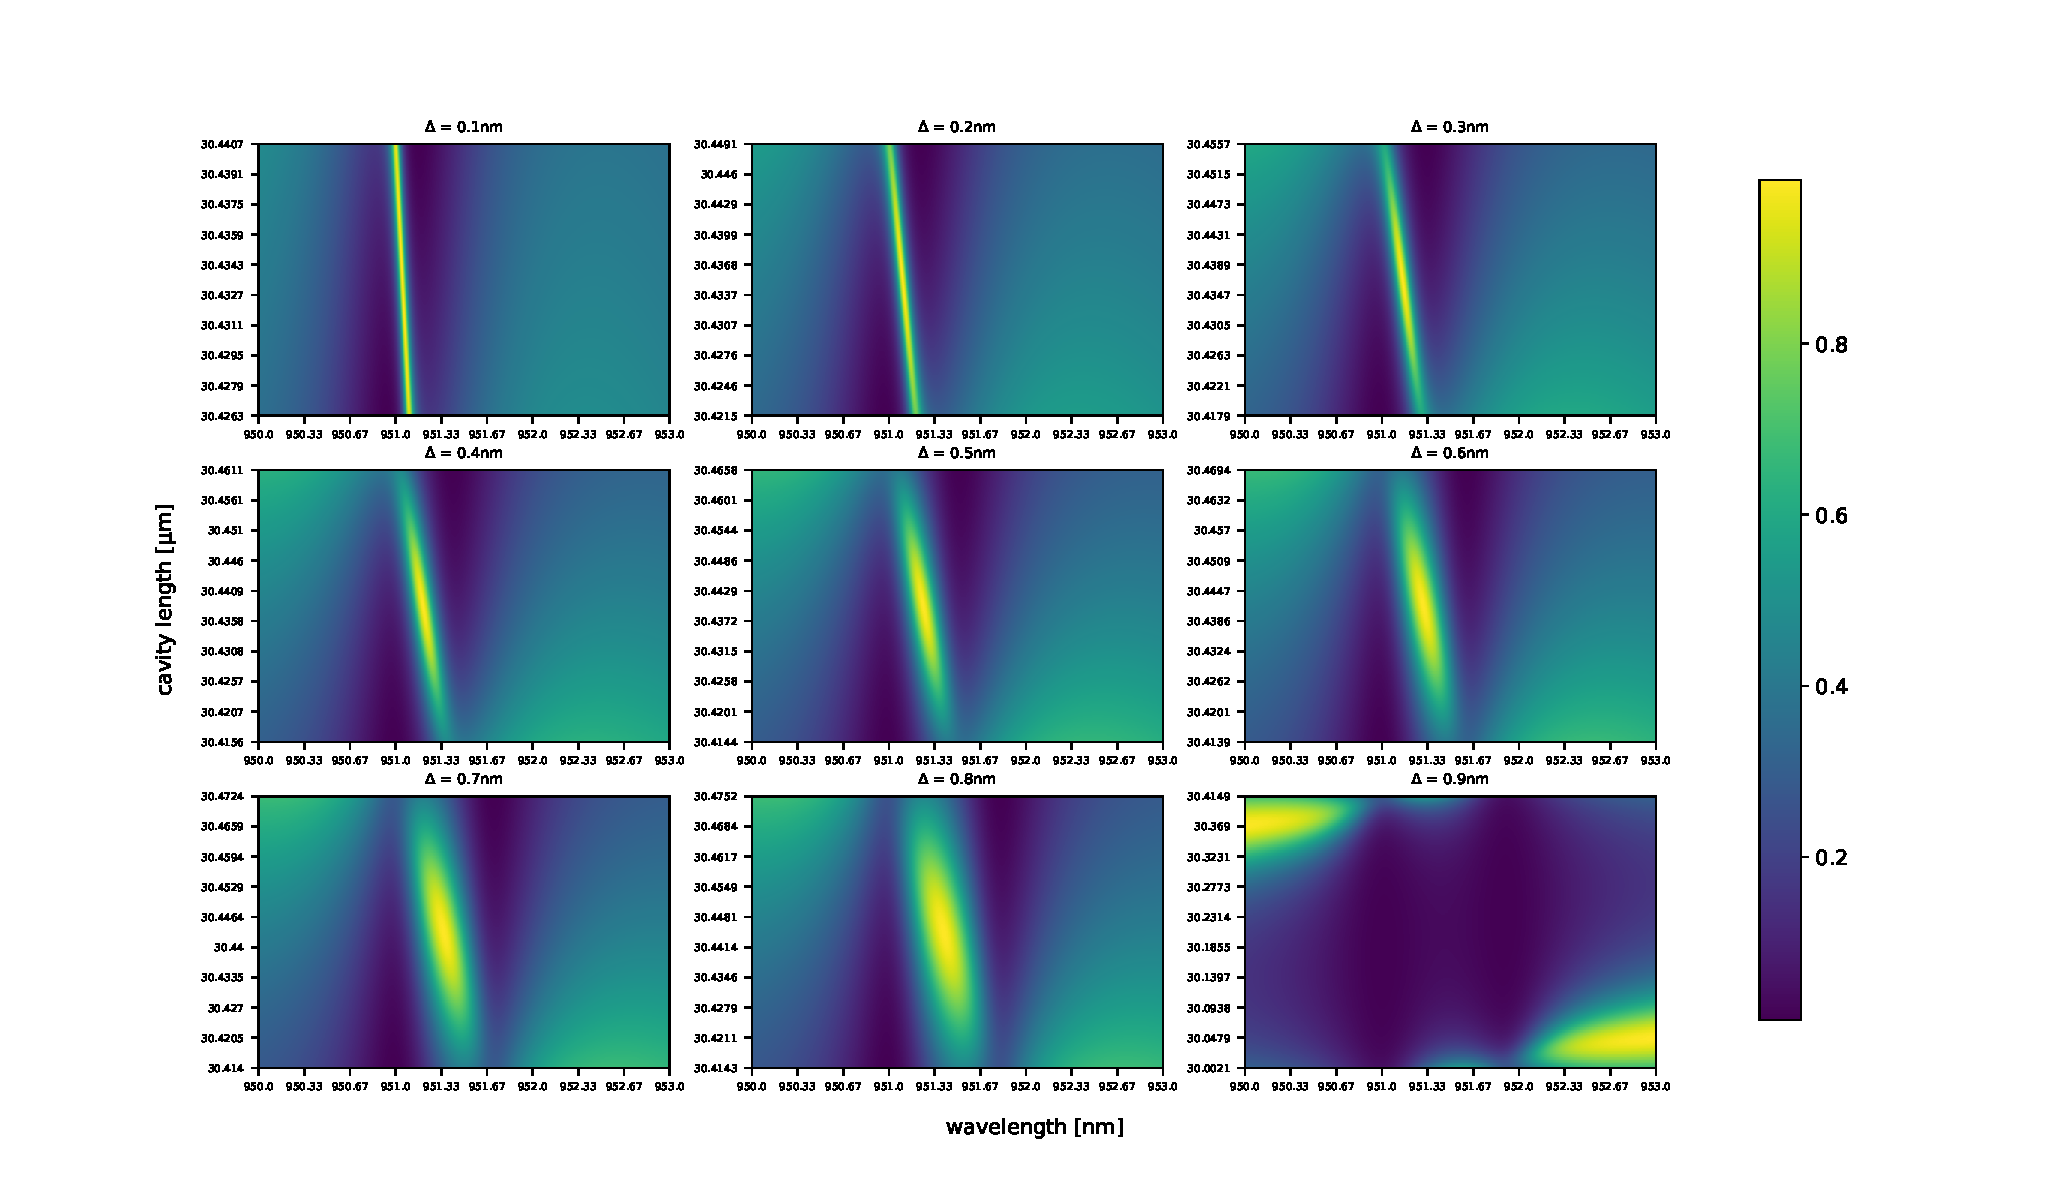
\includegraphics[width=0.95\textwidth]{figures/cmaps_detuning_30um.pdf}
    \caption{Series of heat maps showing lossless double Fano transmission spectra as a function of the cavity length, for increasing detuning $\Delta$.}
    \label{fig:cmaps_detuning}
\end{figure}



%\newpage
%\input{Resumé}

\newpage
\section{References}
\printbibliography[heading=none]
%\newpage
%\input{APPENDIX}
\end{document}

